%% LyX 2.1.4 created this file.  For more info, see http://www.lyx.org/.
%% Do not edit unless you really know what you are doing.
\documentclass[unicode,pdfcover]{scutthesis}
\usepackage{fontspec}
\usepackage{color}
\usepackage{array}
\usepackage{longtable}
\usepackage{graphicx}
\usepackage[unicode=true,
 bookmarks=true,bookmarksnumbered=true,bookmarksopen=false,
 breaklinks=false,pdfborder={0 0 1},backref=false,colorlinks=true]
 {hyperref}
\hypersetup{pdftitle={硕士论文标题},
 pdfauthor={张锟},
 pdfsubject={多尺度遥感图像目标自动检测与识别技术研究结题报告},
 pdfkeywords={关键字1, 关键字2},
 unicode=false,linkcolor=blue, anchorcolor=black, citecolor=olive, filecolor=magenta, menucolor=red, urlcolor=magenta, pdfstartview=FitH}
\hypersetup{hidelinks}
\makeatletter
\providecommand{\LyX}{\texorpdfstring%
  {L\kern-.1667em\lower.25em\hbox{Y}\kern-.125emX\@}
  {LyX}}
\providecommand{\tabularnewline}{\\}
\makeatother
\usepackage{listings}
\usepackage{xunicode}
\renewcommand{\lstlistingname}{列表}

\begin{document}

\title{多尺度遥感图像目标自动检测与识别技术研究结题报告}
\author{余翔宇、秦慧平、刘琲贝、曾群期、张锟、伍冠中、范子娟、陈润泽、陈自清、谢裕麟}
\maketitle
\frontmatter
\tableofcontents{}
\mainmatter
\chapter{绪论}
\section{课题背景}
随着航空航天技术的不断发展,遥感技术水平也在不断革新。由于遥感技术的优越性,遥感技术已广泛应用于多个领域。未来十年,随着遥感图像的各项指标的提高,遥感技术有望进入实时快速地提供各类地球观测数据的新阶段。在遥感图像的基础上,目标识别的信息处理技术是当今自动目标识别的关键技术之一,也是遥感信息提取的核心所在。它在军事和民用领域都具有重要的应用意义和研究价值。自动目标识别技术可以从遥感图像的复杂背景中自动提取目标特征,并根据特定区域和典型目标的特征模板数据库,或利用边缘、灰度、纹理结构等信息实现检测、拦截、识别和跟踪目标。虽然图像处理、模式识别和计算机视觉技术的快速发展为遥感图像目标识别技术的改进创造了条件,但目前遥感图像目标识别技术还不够成熟,与实际应用的要求仍存在较大差距,还有许多问题亟待解决。

首先,遥感图像中的目标具有多样性和复杂性,即遥感图像存在着丰富的信息,待检测的目标的类型和结构复杂多样。它包括河流、湖泊、森林等自然物体,以及建筑物、公路、居民区等人造物体。同时,在遥感图像,待检测物体与其他物体之间会出现重叠等现象,这给遥感图像的目标检测和识别带来了困难。其次,遥感图像中噪声、光照变化、云雾的干扰可能导致同类目标的类内差异增大,不同类型目标的类间差异减小,从而降低了目标的识别精度,给自动识别带来困难。此外,遥感图像的内容复杂,目标来源多样,仅采用低阶特征提取方法无法充分准确地表达遥感图像的目标,限制了遥感图像目标识别的准确性。最后,图像语义信息的处理技术还不够成熟,低层次特征与高层次语义信息难以结合,缺乏有效的先验信息,制约了目标识别精度的进一步提高,这对遥感图像目标识别技术的研究提出了更高的挑战。

目标检测作为计算机视觉中的重要任务,可以从高分辨遥感图像所涵盖的场景中对目标进行准确定位和类别划分,有助于更好的理解图像,在军事战争、农业生产以及城市规划建设等方面都能发挥关键作用。传统的目标检测技术依靠人工设计出的特征算子来进行特征提取,之后再通过滑动窗口的方式用分类器对图像各个子区域进行分类判断,面对简单图像场景下的特定目标检测可以达到不错的效果。但是高分辨率遥感图像中的背景复杂,目标和背景之间的区分度低,并且需要检测的目标种类多样,传统目标检测技术存在这很大的局限性。近年来深度神经网络的兴起以及在图像处理领域的卓越表现吸引了极大的关注,深度神经网络不需要针对特定目标设计特征算子,而是依靠网络自身学习自动化地从图像中提取有用的特征用于后续处理,并且不需要对图像区域进行重复计算,相比于传统方法具有更好的泛化性能,不论是性能还是效率都获得了大量的提升。因此,将深度神经网络用于高分辨率遥感图像目标检测是实现遥感信息自动化处理的重要开端。
  \section{拟解决的关键问题}
从理论的角度分析,与通用的图像目标检测问题相比,遥感图像目标检测具有以下待解决的关键问题:

1. 小目标问题:本文所提出的遥感目标检测方法,主要以可见光遥感图像作为重点研究对象。众所周知,可见光遥感图像一般借助于航空航天设备如卫星、无人机等获得,因此其拍摄位置往往位于数千米高空之中,而特别地,在常见的遥感图像待检测目标中,有诸多尺寸较小的目标如小型车辆(Small Vehicle)、船只(Ship)等,其在遥感图像当中所占尺寸远小于其他目标,同时相比于通用目标检测中的类似目标,其在遥感图像中所占据的像素尺寸依然是较小的,显然地,在遥感图像的目标检测方法中,这一类目标将比网球场(Tennis Court)、码头(Harbor)等大型目标更加难以检测,如何提高对此类小型目标的识别与检测精准度与效率就成为算法设计中一个不可忽视的问题。

2. 目标密集性问题:由于遥感图像取自于高空之中,其往往尺寸较大,能覆盖到非常广阔的地面范围,包含有大量的地面建筑与设施,显然待检测目标并不会均匀地分散在整个图像当中,而是在某些设施中,可能会聚集着大量的待检测目标,最常见的当属停车场、码头与机场,在这三类地面建筑与设施中,分别会聚集有大量的小型车辆、舰船与飞机,体现在遥感图像当中,即这些目标会集中在一片小型区域之中,这就是遥感图像的目标密集性问题。由于现有的检测方法往往是基于“检测+识别”的思路,在检测阶段,过于密集的目标会使得目标检测框产生过分堆积,若不加以鉴别区分,则很有可能让原本正确的检测框在后续处理中因过多重叠被剔除,进而影响检测效率与精准度。

3. 尺度多样性问题:在遥感图像中,存在各种尺度的待检测目标,对于多类型的目标检测方法而言,待检测目标间的尺度多样性成为必须考虑的问题。在传统单一目标检测方法中,会使用预先定义好的输入图像,结合预先设置的尺度网络,得到固定尺寸的特征图像与后续矢量。但在遥感图像中,既有足球场这种大型的目标,也有十字路口、网球场等中型的目标,更多的,还是车辆船只等小型的目标,倘若只使用单一固定尺度大小的检测网络,必然会导致网络对某一类尺度目标的响应远大于其他目标,这是由神经网络的工作方式所限制的,因此,为了得到尽可能好的目标检测效果,必须考虑网络对于多尺度目标的检测方法,即网络必须使用多尺度结构以满足不同目标的检测与识别需求。

4. 视角特殊性问题:常见的通用目标待检测图像往往是基于地面水平方向获取得到,如人脸检测、车辆检测、文字检测等,因此在设计此类通用目标检测方法之时,多会从目标的水平视角特征入手进行检测,但对于高空遥感图像而言,其为俯视角,以车辆检测为例,在水平视角车辆检测方法中,会针对车辆水平外观特征进行学习,然而在遥感图像中,这一特征是不可获取、不可知的,因此需要针对遥感图像中的待检测目标选取更加符合其俯视视角的特征进行学习,这就涉及到对网络感受野与结构,必须依据这一特殊性进行设计。高分辨率遥感影像中的目标通常具有尺度变化较大、视角特殊、方向多变和背景复杂等特点,当前通用的目标检测和识别方法对于此类任务的表现较为一般,体现在其检测精度不高、适应性差,难以胜任遥感目标检测与识别任务。因此,针对遥感图像的多尺度、多方向目标,提出具有针对性的目标检测与识别方法是非常必要的。

5. 方向多样性:遥感图像获取时的俯视视角让所有目标近乎是在同一水平线上,处于不同位置的目标会产生不同的旋转角。而自然图像中的目标如行人、人脸和车辆等都是和水平面垂直分布,一般具有确定的方向。以人脸检测为例,人脸五官在空间方向上往往具有一定的规律,而这种方向上的的规律也可以被用作检测中的一类特征;行人、车辆等目标大多都是垂直于水平面的;遥感图像检测则需要对目标的不同方向具有特征适应性。

\subsection{研究内容}
面对上述提出的关键性问题,课题组内研究人员分别进行了相关的理论研究,并对得出的解决方案进行了详细的实践验证。
具体的研究内容主要由以下4个部分组成:
\begin{itemize}
  \item 遥感目标多尺度检测网络研究
  \item 遥感目标多方向性检测研究
  \item 遥感目标多层次特征提取研究
  \item 遥感目标分割问题研究
\end{itemize}
本文以下章节将会针对这些研究内容提出解决方案并分别进行详细的论述。

\section{数据集}
随着深度学习方法在遥感图像目标检测之中的发展与应用,各类遥感数据集也应运而生。针对遥感图像中有方向目标的检测方法研究,本文使用了两个常见的遥感图像公开数据集DOTA和HRSC2016来进行对比实验。

在DOTA数据集提出之前,已有各种遥感数据集可供研究者使用,其中使用较为广泛的有HRSC2016\cite{liuhigh}数据集,HRSC2016是由西北工业大学刘子坤团队制作的专门用来进行船舶检测的数据集,图像来源于GoogleEarth,总共有1061张图片,包含了海上船舶和近海船舶在内的两种不同场景。它的图片分辨率大小跨度没有DOTA大,从300×300到1500×900,并且大部分图片都是在1000×600左右,数据集中大约有436张图片作为训练集,181张图片为验证集,剩余的444张为测试集,比例大致为4:2:4。数据集图片中的船舶目标也都是由旋转框来进行标注的,所有图片都进行了标注,大部分的船舶目标长宽比值都比较大,达到了7:1。

DOTA数据集\cite{xiadota}是武汉大学夏桂松与华中科技大学白翔等人在2018年共同提出的多目标遥感数据集,其主要数据来源为GoogleEarth和两颗中国卫星GF-2,JL-1,共包含有15类待检测目标与共计2806张遥感图像,这15类目标分别为飞机、船只、储蓄罐、棒球场、网球场、篮球场、田径场、码头、桥梁、大型车辆、小型车辆、直升飞机、足球场、环形路口、游泳池,在每一幅图像中都含有大量的实例,针对实例采用了矩形框进行标注,按顺时针方向依次记录标注框坐标,同时对目标的检测难易度进行了划分。在2019年,DOTA数据集进行了填充与改进成为DOTA1.5,其检测目标由原来的15类增加到16类,添加了对于集装箱起重机的标注信息,同时补全了部分在原数据集中缺漏的实例标注。

在使用DOTA数据集之前,首先必须针对数据集的特殊性进行分析,这样有助于对数据进行预处理,避免引入无关因素影响检测与识别方法的性能,DOTA数据集具有如下几个差异性:

1.样本分布差异。虽然在DOTA数据集中对多类目标进行了标注,但由于实际遥感场景的限制,在数据集中,部分较大尺度目标数量稀少如足球场,而小型车辆类目标确广泛地存在于每幅遥感图像之中,这就导致小型车辆目标数量过多,进而在汇集其标注信息时,容易造成训练时的溢出与显存不足(Out Of Memory, OOM)问题;

2.尺度分布差异。在DOTA数据集中有数千幅遥感图像,但其原始尺寸从$800\times 1000$到$9000\times 6000$皆有,存在显著的尺度分布差异,而神经网络往往只对特定尺寸范围的输入具有良好响应。因此,在使用DOTA数据集进行实验与评估时,一种确保网络输入尺寸一致性的方法是很有必要的;

3.采样距离差异。与OGST(Oil and Gas Storage Tank Dataset)数据集\cite{rabbi}等具有固定采样距离的数据集不同,由于DOTA使用的遥感图像来源多样,因此其标注中带有不同的采样距离参数,另外还存在部分图像采样距离缺失。值得注意的是,采样距离与分辨率共同决定了一幅遥感图像所覆盖的实际地面区域大小,因此,在进行地面目标检测时,这两类因素都将对待检测目标尺度产生影响。

针对这些差异性,在文章中分别使用了针对性的处理方法进行优化,如针对小型目标过多导致的OOM问题,可以使用筛选与增广的方式调节网络在一次学习中所使用的的标注真实样本数量;针对尺度的多变,可以使用裁剪与拼合的方式进行一致性处理;针对采样距离的差异,则设计了对采样距离敏感的卷积网络结构来进一步引入预测信息辅助识别。

\chapter{项目成果总结}
通过本基金项目,我们课题组取得了一系列的成果,其中包括:

1. 一篇已发表的论文,标题为《ROSD: Refined Oriented Staged Detector for Object Detection in Aerial Image》,发表于IEEE Access。该论文作者为张锟、曾群期及余翔宇。这篇论文详细介绍了课题组的两个研究成果,包括改进的多方向级联目标检测方法与基于特征对齐和目标长宽比的目标检测方法,通过对这两个方法进行详细的推导论述,搭配详尽的实验过程介绍及结果展示,这篇论文得以被接收。

\begin{figure}
\centering{}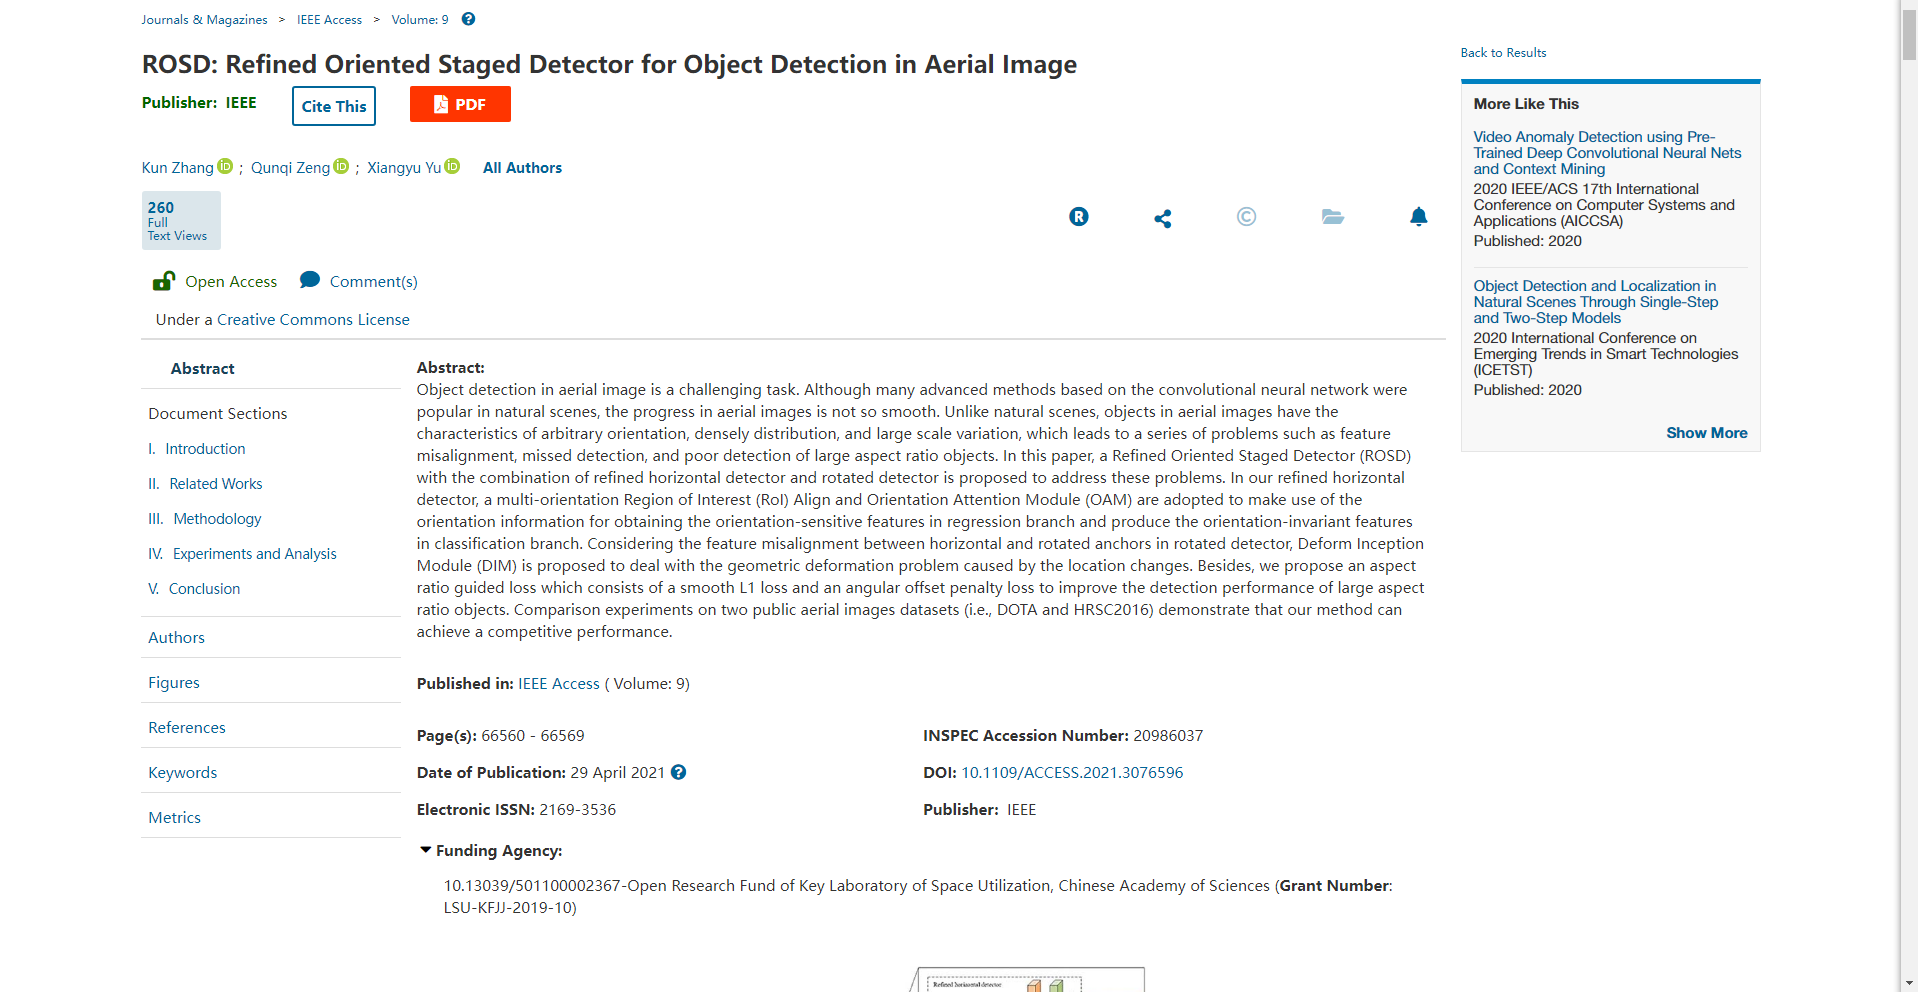
\includegraphics[scale=0.3]{figure/IEEE.png}\caption[短标题]{\label{fig:IEEE1截图}张锟IEEE Access论文截图}
\end{figure}

2. 课题组当前有一篇审稿中的IEEE Access论文,论文标题为《Object Detection in Aerial Image with Ground Sample Distance Super-Resolution》。该论文作者为曾凯与曾群期。这篇论文详细介绍了课题组的另外两个研究成果,包括了改进的深度级联遥感目标检测网络以及基于遥感图像GSD预测的超分辨遥感目标检测方法。

\begin{figure}
\centering{}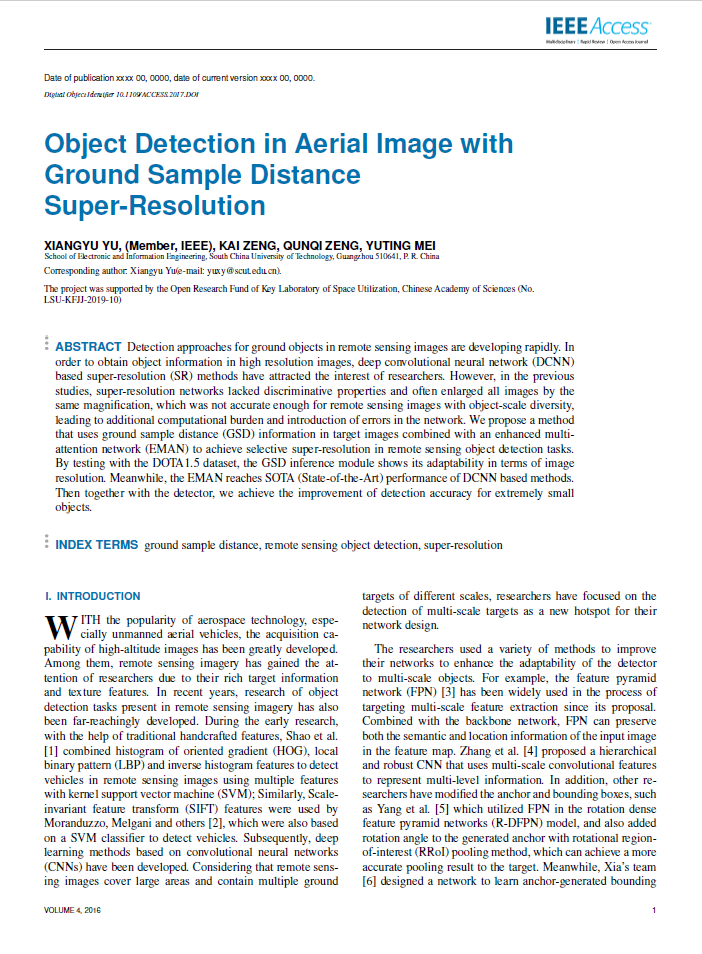
\includegraphics[scale=0.6]{figure/曾凯IEEE截图.png}\caption[短标题]{\label{fig:IEEE2截图}曾凯与曾群期IEEE Access论文截图}
\end{figure}

上述两篇论文均已标注 The project was supported by the Open Research Fund of Key Laboratory of Space Utilization, Chinese Academy of Sciences (No.LSU-KFJJ-2019-10)。

3. 课题组成员张锟和曾群期分别基于这个基金项目各自编写了一篇硕士毕业论文,完成了硕士期间的学习和工作内容。

\begin{figure}
\centering{}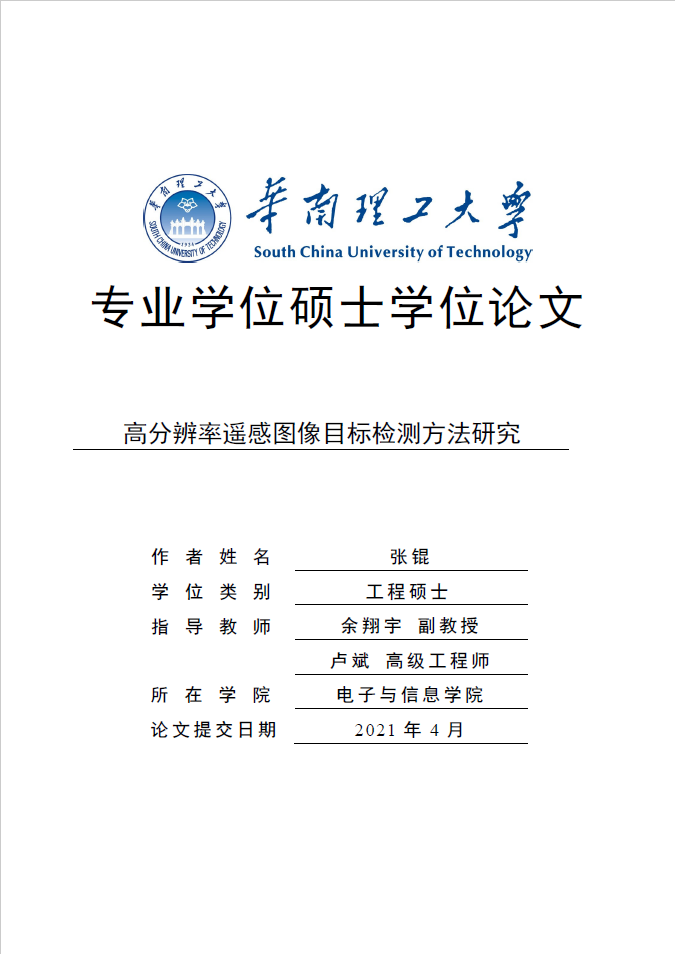
\includegraphics[scale=0.45]{figure/张锟毕业论文截图.png},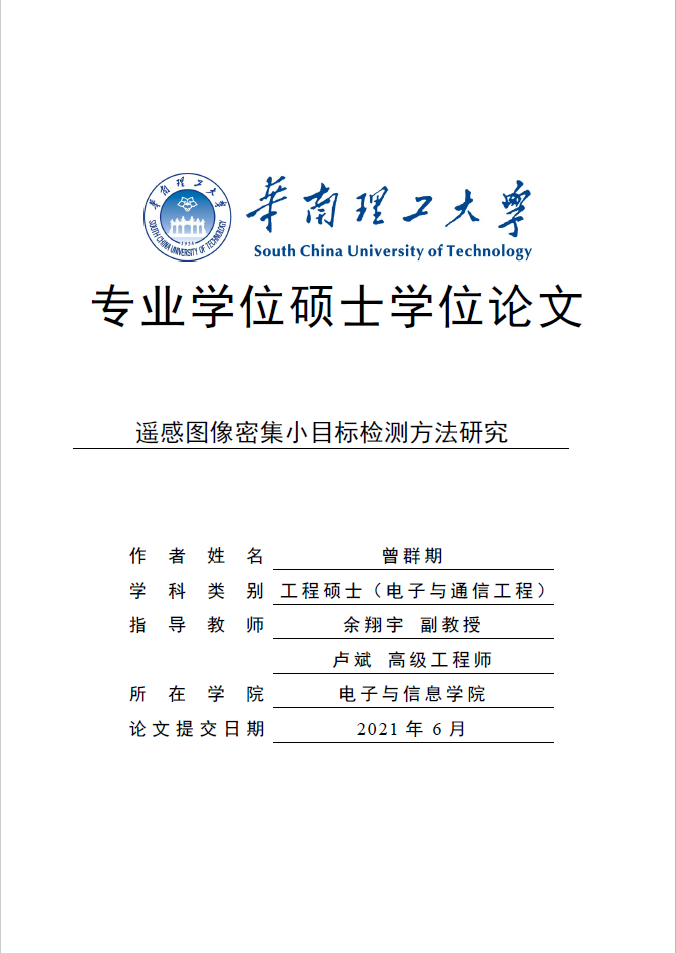
\includegraphics[scale=0.45]{figure/群期毕业论文截图.png}\caption[短标题]{\label{fig:毕业论文截图1}张锟及曾群期毕业论文截图}
\end{figure}

4. 课题组成员张锟和曾群期分别基于这个基金项目各自发表了一篇专利。
\begin{figure}
\centering{}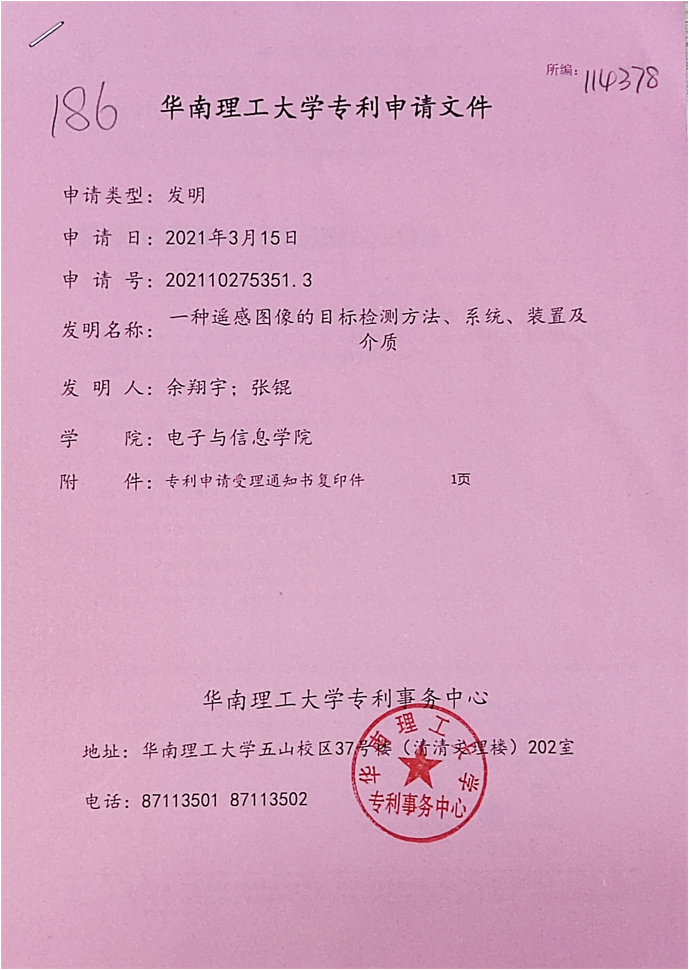
\includegraphics[scale=0.3]{figure/张锟专利.png},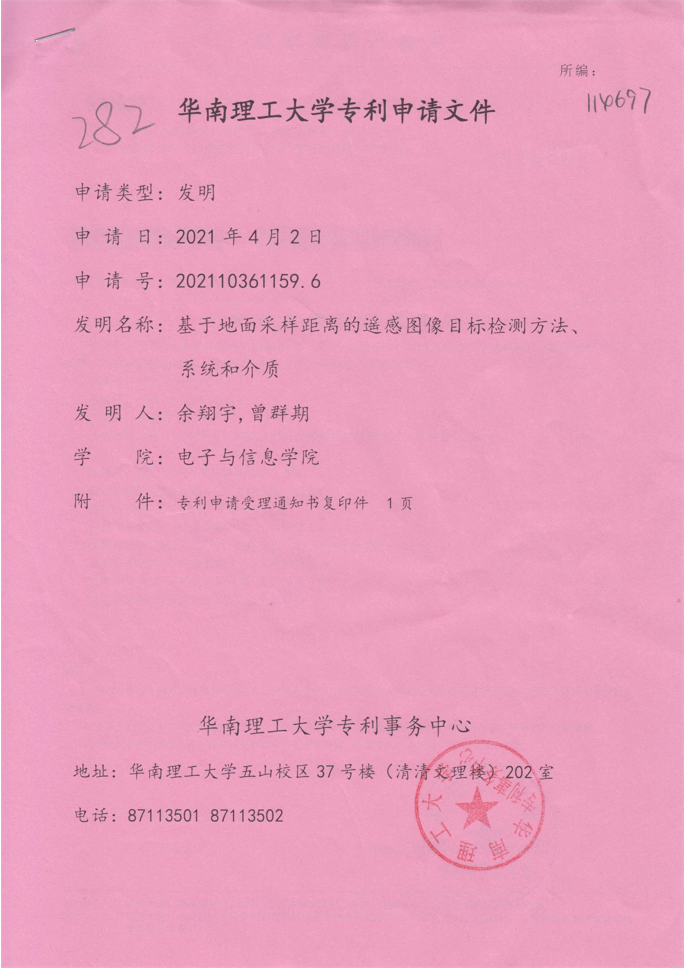
\includegraphics[scale=0.3]{figure/群期专利.png}\caption[短标题]{\label{fig:毕业论文截图1}张锟及曾群期专利截图}
\end{figure}

\chapter{遥感目标多方向性检测研究}


\section{引言}

根据绪论章节中提出的研究内容,与常规目标检测算法的对象不同,由于航空遥感图像中的各类目标是位于近似同一水平面上,因此其通常会具有多个方向。
在高分辨率遥感图像中,由于获取图像时的俯瞰视角,待检测的目标在图像中是密集分布和方向多样的,并且由于获取位置往往是几千米的高空,图像中的小目标最小到只有十几个像素大小。基于传统水平框检测的目标检测方法在面对高分辨率遥感图像时会碰到很大的问题,相邻目标的水平检测框之间会存在大部分的重叠,一方面会对检测过程中候选区域框的特征提取带来干扰,另一方面在使用非极大值抑制对部分检测框进行滤除时可能会过滤掉一些相邻目标的正确预测框,极大的影响了检测目标的召回率。因此,如何应对高分辨率遥感图像中小目标密集分布且任意朝向的特点,设计改进的检测方法,提升模型表现,成为了亟待解决的问题。

这一章节的内容主要是解决了遥感目标多方向性检测研究的问题,本章提出了一种改进的多方向级联R-CNN目标检测方法,设计了一种两级级联的检测网络,第一级检测网络完成水平感兴趣区域到旋转感兴趣区域的转换,第二级检测网络对旋转区域进行特征提取做进一步的检测框的精确定位。在第一级检测结构提出了多方向RoI对齐结构获取方向敏感特征用于回归,同时在回归分支设计了方向注意力模块来对方向信息进行增强。另外考虑到分类和回归任务对于方向敏感的不一致性,在分类分支将方向敏感特征做了平均池化来获取适合分类的方向不变特征。

在基于区域提取的目标检测方法中,检测过程由两部分组成,第一部分先在特征图每个位置生成不同尺度和长宽比的候选区域,经过RPN调整候选区域位置得到可能包含目标的感兴趣区域,第二部分是由分类和回归分支组成的检测网络,逐个对RPN得到的感兴趣区域提取特征,输入检测网络进一步对是否存在目标和目标精确位置进行判断。在一般情况下RPN和检测网络的输入图像特征图是一样的,这样的设定没有考虑到生成的候选区域和RPN调整得到的感兴趣区域之间的位置发生了偏移,导致特征点位置也发生了变化,使用相同的特征图会使得提取的感兴趣区域的特征不够准确,影响后续的检测网络。

另外,我们在研究中发现,模型对于不同长宽比的检测目标得到的有方向检测框的结果有明显的的差距,在其它参数保持不变的情况下密集分布的小长宽比的目标的漏检率会远远小于大长宽比的目标,而且小长宽比的目标得到的检测框和数据集中标注的框之间的IoU值也比大长宽比的目标要好。这意味着模型在训练过程中没有对不同长宽比之间的角度偏移参数进行充分平等的学习,小长宽比目标的角度偏移量学习在实际情况下的表现更好。

针对这个问题,本章还提出了一种基于特征对齐和目标长宽比的方法,首先利用了可形变卷积具有显著地几何形变建模能力的特性,基于可形变卷积设计了一个多分支结构来进行特征对齐,并且通过不同扩张率的空洞卷积对感受野进行扩增以适应不同层次的检测目标,其次在训练模型对损失函数进行了改进,以目标长宽比比值作为控制系数,让模型在训练阶段在角度偏移的学习上更加注重大长宽比的目标,以此来提高模型对于大长宽比目标的检测精度。通过这种组合的方法,我们有效地提高了对于遥感目标多层次特征提取的效果。

\section{算法设计}

图\ref{fig:4-1}是本章提出算法的总体结构,该图展示了在基于区域提取的Faster R-CNN算法上所做的改进。在特征提取阶段,将ResNet作为基础网络,为了应对高分辨率遥感图像中的小目标和尺度差异大的问题,使用了FPN结构将低层的定位信息和高层的语义信息进行融合加强特征表现。在检测阶段,将原有的水平框检测器替换为本章提出的两级级联有方向检测器,包括使用了有方向检测框代替了传统的水平检测框、设计的多方向RoI对齐模块和方向注意力模块。为了应对旋转感兴趣区域和水平感兴趣区域之间的特征不对齐问题,对于FPN每一层输出的特征图,在输入第二级检测网络之前,先采用了多分支特征对齐模块对特征图调整,使得提取的旋转感兴趣区域的特征能够更好的表示被检测的有方向目标,同时在两级的检测网络结构中都采用了基于目标长宽比的损失函数来加强模型对于不同长宽比目标的检测精度。

%\begin{figure}
%\centering{}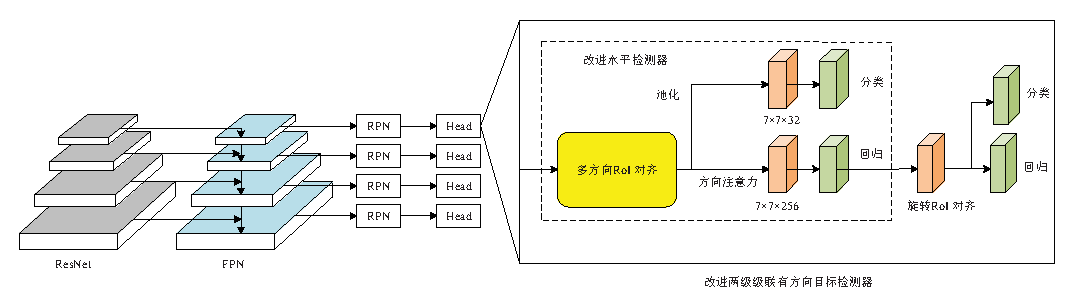
\includegraphics[scale=0.9]{figure/3-1}\caption[短标题]{\label{fig:3-1}改进的多方向级联R-CNN目标检测方法结构示意图}
%\end{figure}

\begin{figure}
\centering{}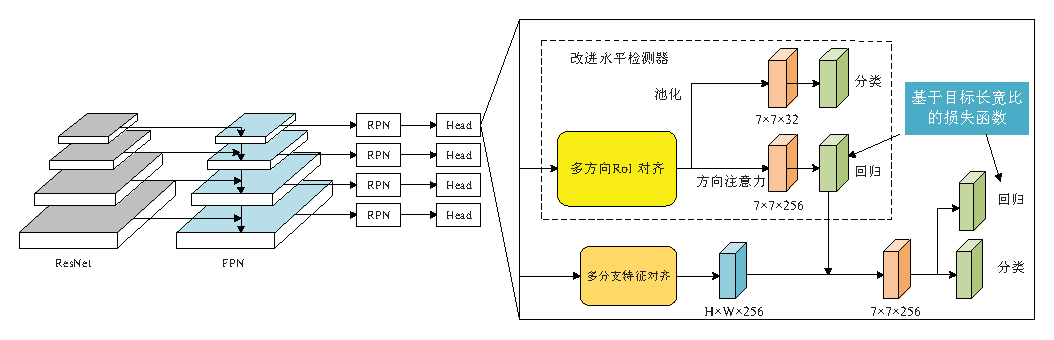
\includegraphics[scale=0.9]{figure/4-1}\caption[如果图题太长,在这里写个短标题只在图索引中出现]{\label{fig:4-1}改进的多方向级联R-CNN目标检测方法结构示意图}
\end{figure}

\subsection{有方向检测框}

近年来自然图像中的基于水平框检测的目标检测方法取得了巨大的成功,在检测精度和速率上都有了长足的进步。不同于自然图像,水平框检测在面对高分辨率遥感图像会碰到这样的问题:图\ref{fig:3-2}所示为同一副图像中真实标注的水平框和有方向框之间的对比情况,当采用\ref{fig:3-2} (a)所示的水平框对密集分布的小目标进行检测时,相邻目标之间的检测框非常容易发生重叠,在检测阶段进行非极大值抑制滤除部分检测框时,阈值难以界定,过低的阈值会使得很多有效的检测框因为和相邻目标的检测框之间有重叠而被滤除,过高的阈值会使得最终的检测结果中遗留下了很多的实际效果不好的检测框,严重影响到了目标的召回率和精确率,进而降低了模型表现。而当采用图\ref{fig:3-2} (b)所示的有方向检测框进行检测时,相邻目标之间的检测框的重叠情况得到了很好的改善,非极大值抑制阶段的问题可以很好的解决,能够有效提升检测性能。

\begin{figure}
\centering{}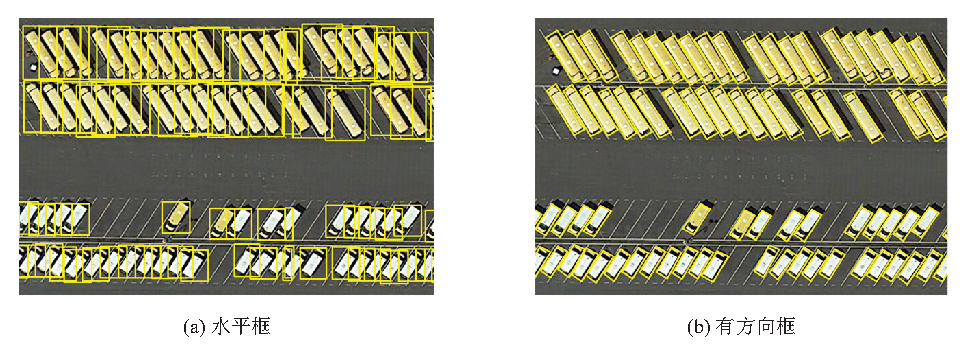
\includegraphics[scale=0.9]{figure/3-2}\caption[短标题]{\label{fig:3-2}水平检测框和有方向检测框对比}
\end{figure}

如图\ref{fig:3-3} (a)所示,基于自然图像的目标检测方法采用水平框对目标位置进行定位时使用的参数为(\emph{x}, \emph{y}, \emph{w}, \emph{h}),其中(\emph{x}, \emph{y})指的是框的中心,\emph{w}和\emph{h}指的是水平框的宽和高,训练阶段将这4个参数量的偏移作为回归分支的预测值进行训练。而本章的方法中使用了额外的角度参数来定义有方向检测框,如图\ref{fig:3-3} (b)所示,有方向检测框的参数表示为(\emph{x}, \emph{y}, \emph{w}, \emph{h}, $\theta$),其中角度$\theta$表示的是水平线与检测框长边之间的夹角,此定义下的$\theta$范围为($-\frac{\pi}{2}$, $\frac{\pi}{2}$),当$\theta$ = 0°时有方向检测框也就变成了水平检测框,在本章的两级级联的检测网络中都采用了有方向检测框的参数作为回归分支的预测输出。

\begin{figure}
\centering{}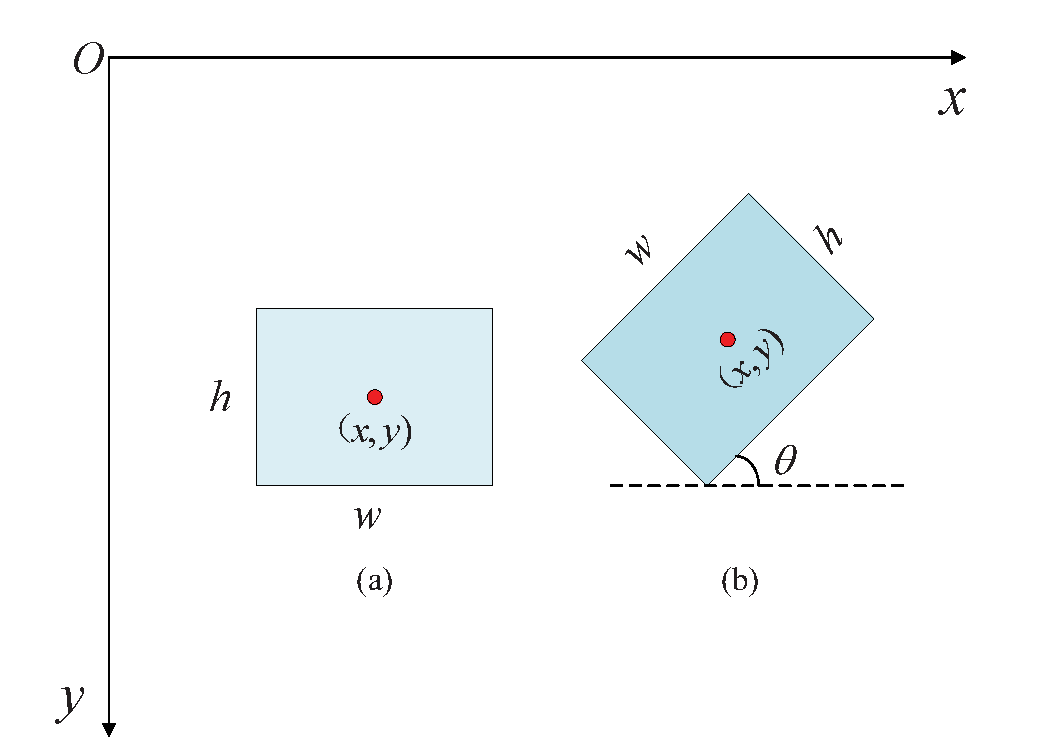
\includegraphics[scale=0.5]{figure/3-3}\caption[短标题]{\label{fig:3-3}两种检测框表示方法:(a)水平框;(b)有方向框}
\end{figure}

\subsection{两级级联检测器结构}

一般情况下,一些基于水平框检测的目标检测方法首先使用深度神经网络对输入图片进行特征提取,然后在候选区域生成阶段特征图每个位置点会生成不同尺度和长宽比大小的锚点框作用于RPN,对锚点框的位置作进一步的调整得到水平感兴趣区域,之后通过使用单级检测器在分类和回归分支对感兴趣区域中的目标位置进行预测。这样的单阶检测器在水平框检测上可以达到比较好的检测效果,但是在进行有方向检测框时,仅仅使用单阶检测器从水平感兴趣区域框中获取待检测有方向目标的特征并对目标的位置作进一步的定位效果欠佳,所提取的特征不仅不能很好地对有方向目标进行表示而且在一些情况下会被周围同类目标的特征干扰。基于这样的问题有一些研究学者采用在候选区域生成阶段生成额外的不同方向的锚点框作为候选区域来表示有方向目标框的位置\cite{li2017rotation}\cite{xia2018dota},这些方法虽然可以提升有方向框目标的检测精度,但是在候选区域生成阶段所产生的锚点框数量较之前有成倍数的增长,又由于RPN网络的正负样本划分和非极大值抑制阶段需要计算两个锚点框之间的IoU,产生的的计算量相较于之前的方法有指数级别的增长。过多计算资源的消耗导致在训练阶段对一些包含较多检测目标的图片进行训练时很容易出现内存溢出的情况,一方面会使得一部分的训练数据得不到充分的学习,另一方面计算量的显著增长使得模型的训练和检测速度非常缓慢,对检测精度和检测效率都有不好的影响。

为了解决上述提到的问题,本文提出了一个两级级联的检测结构来进一步实现对有方向框的检测。这样的两级级联的检测结构不需要在候选区域生成阶段生成带不同方向的锚点框来得到有方向目标位置的准确特征,而是先采用了一个分类和回归检测网络结构对从RPN网络得到的水平感兴趣区域进行调整,筛选出包含目标的感兴趣区域并根据获取的感兴趣区域特征进行第一次有方向框检测回归得到包含目标的旋转感兴趣区域的初步位置,然后再使用另外一个分类和回归检测网络结构,以初步获取得到的旋转感兴趣区域的特征作为输入,进一步对该区域内有方向目标所在的准确位置进行预测,通过这样一个两级级联的检测结构,不仅可以解决因为生成数目过多的锚点框导致的内存溢出问题,而且经过从水平感兴趣区域到旋转感兴趣区域再到有方向目标精确位置这样一个递进的回归过程,一步步地提升了获取的目标位置的特征质量,有效的改善了有方向检测框的检测精度。

\subsection{多方向RoI对齐 模块}

在基于区域提取的目标检测方法中,对候选区域的特征提取是检测环节中极为重要的一环,只有提取出能够很好的表示候选区域中所包含目标的特征才能让后续的分类和回归任务更精确地进行。在自然图像的目标检测算法中经常用到的特征提取方法为RoI对齐,将从RPN网络中获取得到的水平感兴趣区域通过划分单元格、特征点采样和双线性插值的过程输出为固定尺度大小的特征图,以此作为每个感兴趣区域的特征表示,再将其输入到分类和回归分支对每一个感兴趣区域是否包含目标以及目标的具体位置进行学习预测。

然而,不同于自然图像,由于高分辨率遥感图像中目标密集分布的特性,在进行有方向检测框的任务时对于感兴趣区域的特征提取有了更高的要求。如图\ref{fig:3-4} (a)所示,红色实线框为标注的有方向检测框,黄色虚线框为标注的水平检测框,绿色虚线框为RPN网络中输出的水平感兴趣区域框,结合图\ref{fig:3-4} (a)和图\ref{fig:3-4} (b)能够看出,RPN输出的感兴趣区域框与实际标注的水平框之间存在偏移,一方面没有将待检测目标完全包括在内,另一方面由于目标的密集分布特性,待检测目标相邻的同一类的目标也被包含在内。如果使用之前提到的传统RoI对齐提取特征会忽略掉这样的问题,导致提取出的特征并不能很好的表示目标并且会被相邻目标的特征所干扰,输入到分类和回归分支的特征受到影响不能进行充分的学习,进而影响了对感兴趣区域中有方向目标的进一步定位。

针对上述的问题,在本章的方法中提出了多方向RoI对齐模块,如图\ref{fig:3-4} (c)所示,不直接对RPN网络中输出的水平感兴趣区域进行特征提取,而是先将该感兴趣区域进行多个不同角度的旋转,得到形状大小一样但是方向不同的带旋转角度的区域,也就是图\ref{fig:3-4} (c)中的蓝色实线框。可以看到经过一定角度的旋转之后,带旋转角度的区域可以更好的包括待检测目标,对于相邻的同类目标也有一定的滤除作用,并且不同角度方向的区域对于同一目标能提取到的特征也不一样,使得各个方向上的旋转区域可以更好的表示出待检测目标的特征。之后再在对应通道的输入特征图单独提取每个方向上的旋转区域特征并拼接在一起组成方向敏感的目标特征表示,具体的操作流程如下:

\begin{figure}
\centering{}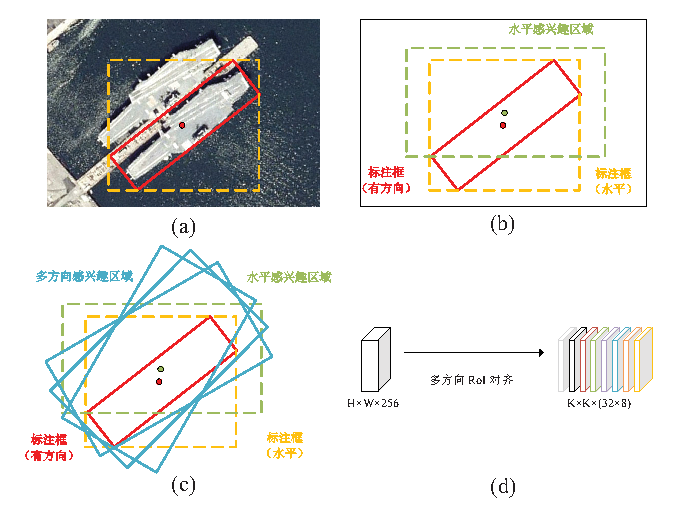
\includegraphics[scale=1.0]{figure/3-4}\caption[短标题]{\label{fig:3-4}多方向RoI对齐的思路流程:(a)带标注框的原始图像;(b)水平感兴趣区域与有方向目标标注框之间的偏移;(c)不同角度旋转水平感兴趣区域;(d)多方向RoI对齐输出}
\end{figure}

给定大小为\emph{H}$\times$\emph{W}$\times$\emph{C}大小的特征图和水平感兴趣区域框(\emph{x}, \emph{y}, \emph{w}, \emph{h}),(\emph{x}, \emph{y})表示框的中心点坐标,\emph{w}和\emph{h}分别表示框的宽和高,多方向RoI对齐首先在此基础上生成\emph{N}(\emph{N}默认为8)个不同方向上的旋转感兴趣区域框,然后使用旋转RoI对齐提取每个方向上框的特征,最后的输出特征为\emph{K}$\times$\emph{K}$\times$($\frac{C}{N}$ $\times$\emph{N}),\emph{K}$\times$\emph{K}表示的是我们将旋转框分成的单元格数目,通常来说K的大小为7,因此,对于每个索引为(\emph{i}, \emph{j})(0$\leq$\emph{i}<\emph{K}, 0$\leq$\emph{j}<\emph{K})的单元格,提取出的特征为
\begin{equation}
  y_{c^n}(i,j)=\sum_{(x_h,y_h)\epsilon{bin(i,j)}}F_{i,j,c^n}(\varphi(x_h,y_h))/s_{i,j}
\end{equation}

\begin{equation}
  \theta=-\frac{\pi}{2}+n\frac{\pi}{N},c^n\epsilon[n\frac{C}{N},(n+1)\frac{C}{N}),n=0...,N-1
\end{equation}
其中$F_{i,j,c^n}$表示的是对应通道为$c^n$的特征图上索引为(\emph{i}, \emph{j})的单元格特征,对于输入的\emph{H}$\times$\emph{W}$\times$\emph{C}大小的特征图,先按特征图总的通道数\emph{C}将输入特征图按顺序平分为\emph{N}份,在进行特征提取时每一份特征图对应的旋转框的方向也不同,比如说\emph{C}=256,\emph{N}=8,则$c^1$ $\epsilon$[0, 32),对应的角度$\theta$ = -$\frac{\pi}{2}$,即通道数为0到32的特征图提取特征时旋转框的角度为$-\frac{\pi}{2}$。$s_{i,j}$是每一个单元格内的采样点数目,一般情况为4,然后对于水平框中每一个采样点($x_h$, $y_h$),先要通过转换方程$\varphi$将其转换成对应方向的旋转框上的相应位置($x_r$, $y_r$)来表示,转换方程如下:

\begin{equation}
  \binom{x_r}{y_r}=\varphi(x_h,y_h)=\binom{cos\theta \quad -sin\theta}{sin\theta \qquad cos\theta}\binom{x_h-w/2}{y_h-h/2}+\binom{x}{y}
\end{equation}

其中(\emph{x}, \emph{y}, \emph{w}, \emph{h})分别表示的是水平感兴趣区域的中心位置、长和宽,$\theta$为对应框的旋转角度,在得到每个单元格内需要采样的点的位置之后,每个采样点位置的特征值通过双线性插值的方法从邻接位置获取,最后再对所有采样点的特征值求平均得到每个单元格最后的特征表示输出。

基于上述的结果,经过多方向RoI对齐模块,我们可以从RPN输出的水平感兴趣区域框提取得到包含\emph{N}个方向的方向敏感特征,同时考虑到分类任务和回归任务对于方向敏感的不一致性,我们只将方向敏感特征用于回归分支。而对于分类分支,我们旨在通过平均池化方向敏感特征来获取方向不变特征,这可以将\emph{N}个方向通道的特征值取平均来简单完成。分类分支的方向不变特征$x_{cls}$的计算方式如下:

\begin{equation}
  x_{cls}=\frac{1}{N}\times {\sum_{n=0}^{N-1}y_{c^n}}
\end{equation}

通过上述的步骤,我们可以得到多方向的方向敏感特征和方向不变特征分别作为回归和分类分支的输入特征。需要注意到的是方向不变特征相比于之前有着更少的参数,假定输入的特征图大小为\emph{H}$\times$\emph{W}$\times$256,采用的方向数目为8,则分类分支的方向不变特征的大小为\emph{K}$\times$\emph{K}$\times$32,与之前的\emph{K}$\times$\emph{K}$\times$256相比显著减少了后续操作所需的计算量。

\subsection{方向注意力模块}

虽然说我们可以通过多方向RoI对齐模块提取多个不同方向上的旋转框的特征来更好地对待检测的有方向目标进行特征表示,但是我们也不能保证每一个方向上的特征都是绝对有效的。比如说当待检测目标的旋转角度为0°,也就是水平框时,旋转角度过大的旋转框相对于目标位置的偏移会使得提取到的特征不能很好的表示待检测目标,如果以同等贡献来定义该特征和其它方向上的特征在一定程度上会降低对于此类目标的检测性能。

针对上述问题,本章节提出了方向注意力模块来量化每个方向上的特征的贡献,对于不同方向的待检测目标,每个方向上的特征所做的贡献也不相同。图\ref{fig:3-5}展示本章节提出的方向注意力模块的结构图,受SE-Net(Squeeze and Excitation Network)\cite{hu2018squeeze}的启发,我们想对每个方向通道上的特征进行0-1之间的量化,以此来表示每个方向上的贡献。与SE-Net不同的地方在于,我们将全局平均池化结构替换成了组卷积结构,把属于同一个方向的通道特征分为一组,每一组分别进行卷积得到该方向上的特征表示。例如对于输入到回归分支的\emph{K}$\times$\emph{K}$\times$\emph{C}大小的特征图,将\emph{C}个通道的特征分为\emph{N}(与方向数目相等)组,每一组的通道数为$\frac{C}{N}$,组卷积的卷积核大小为\emph{K}$\times$\emph{K},再将\emph{N}组经过组卷积之后的特征拼接在一起,这样处理之后输出的特征图大小为1$\times$1$\times$\emph{C}。之后再经过两层全连接层获取每个方向通道上的量化贡献值,并将量化贡献值和输入的方向敏感特征相乘获取最后的输出,最终经过方向注意力模块得到的输出可以表示为

\begin{equation}
  F_{out}=s*F=\sigma(W_2\delta(W_1 \mathop{groupconv}\limits_{K\times K,group=N}(F)))*F
\end{equation}
其中$\sigma$表示的是Sigmoid激活函数,$\delta$表示的是ReLU激活函数,$W_1$表示的是维度下降的全连接层,维度衰减参数为\emph{r}(默认为16),与之相反$W_2$表示的是维度上升的全连接层,最终维度保持一致,*表示的是将每个方向通道的贡献\emph{s}和输入特征图\emph{F}相乘,也就是最后的输出特征图。

\begin{figure}
\centering{}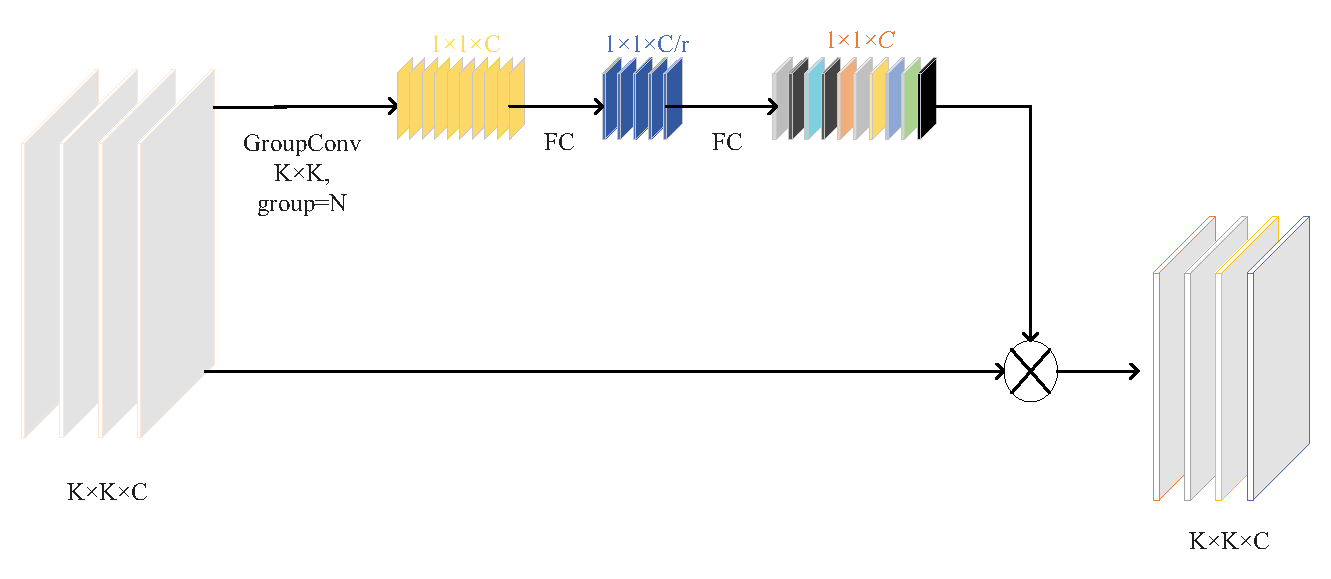
\includegraphics[scale=0.7]{figure/3-5}\caption[短标题]{\label{fig:3-5}方向注意力模块网络结构}
\end{figure}

通过上述的方式,方向注意力模块从本质上可以实现对输入特征进行动态的选择,可以看成是对每个方向通道上的特征做了自注意力机制。将多方向的方向敏感特征作为输入,每个方向的特征自己进行卷积得到该方向的贡献表示来量化每个方向上的重要性,赋予重要性低的方向小的权重,而赋予重要性高的方向相对大的权重,可以根据待检测目标在图像中的方向自适应地调整每个方向的贡献,进一步提升对于方向多样的目标的检测精度。

\subsection{空洞卷积}

在CNN中,感受野的定义是CNN中每一层的输出特征图上的特征点在输入图像中映射的区域大小,即特征图上的一个点对应输入图像上的一个区域。在传统的CNN网络结构设计中,主要是通过在卷积操作中采用大的卷积核或者多个小的卷积核进行堆叠以及池化操作降低特征图的尺寸来达到增大感受野的作用,这样的做法一方面大卷积核和堆叠的小卷积核都产生了额外的计算量,另一方面池化操作会使得空间信息丢失,尤其是小目标来说,在经过几次池化操作之后目标的特征信息甚至不能由特征图上的特征点来表示。

为了能够在不产生额外的计算量和损失空间信息的基础上进行感受野的扩增,Yu等人提出了空洞卷积(dilated convolution)\cite{yu2015multi},和标准的卷积操作相比,空洞卷积在卷积时多定义了一个表示扩张率的超参数\emph{d}来对卷积核进行间隔采样,\emph{d}表示的是卷积核进行卷积时各个位置的间隔距离,当\emph{d} = 1时即为正常卷积,图\ref{fig:4-2}分别展示了卷积核尺寸为3$\times$3,\emph{d}分别为1、2、3时的空洞卷积的示意图,红色的圆点为卷积时卷积核在特征图上的采样位置,图\ref{fig:4-2} (a)所示的\emph{d} = 1时的空洞卷积和普通卷积一样,图\ref{fig:4-2} (b)所示为\emph{d}= 2时的空洞卷积,可以看到通过对卷积核间隔采样,3$\times$3大小的空洞卷积核可以达到5$\times$5大小的普通卷积的效果(红色圆点所围成的区域大小),同理图\ref{fig:4-2} (c)中的\emph{d} = 3时的空洞卷积可以达到7$\times$7大小的普通卷积的效果。在进行空洞卷积的过程中,特征图的大小自始至终都没有产生变化,没有造成空间信息上的损失,并且在达到7$\times$7的感受野也只是使用一个3$\times$3大小的卷积核,没有产生额外的计算量。在应对遥感图像中目标的多尺度问题上,可以使用多个并行的不同扩张率大小的空洞卷积层来获得不同的感受野。

\begin{figure}
\centering{}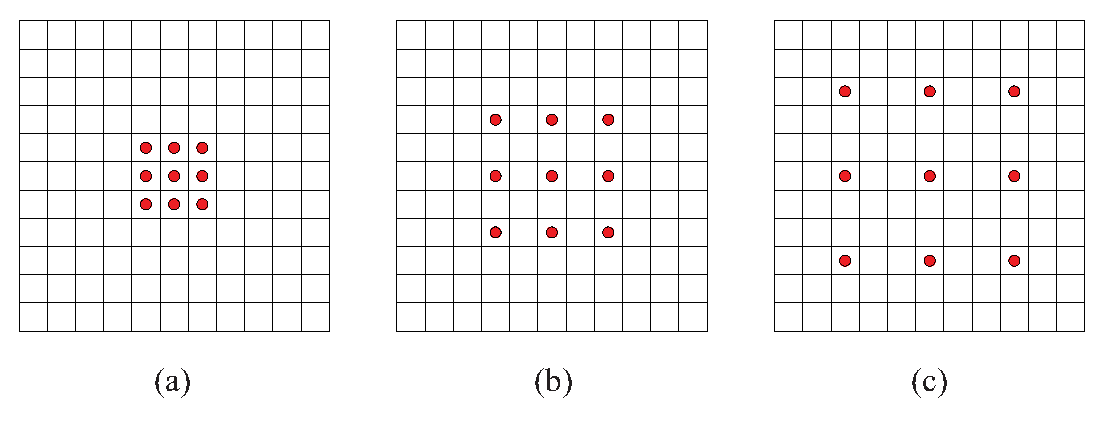
\includegraphics[scale=0.7]{figure/4-2}\caption[如果图题太长,在这里写个短标题只在图索引中出现]{\label{fig:4-2}不同扩张率空洞卷积示意图:(a)扩张率\emph{d} = 1;(b)扩张率\emph{d} = 2;(c)扩张率\emph{d} = 3}
\end{figure}

\subsection{多分支特征对齐模块}

在改进的多方向级联R-CNN目标检测方法中,第一级检测结构对水平感兴趣区域进行了调整,从水平区感兴趣域转变成了旋转感兴趣区域,此时第二级检测结构需要对旋转感兴趣区域进行特征提取做进一步分类和回归,相对于第一级检测结构的水平感兴趣区域,旋转感兴趣区域需要采样的特征点在水平和垂直方向上都有了一定的偏移,如果仍然使用在第一级检测结构中所用到的特征图,采样特征点上的特征值不能很准确的来表示旋转感兴趣区域内的待检测目标。当然,这样的一个位置点的偏移可以看成是几何形变的一种,而可形变卷积在形变问题上有着显著地表现,因此可以将可形变卷积用来处理这样的特征不对齐问题。

可形变卷积在模块中增加了对于空间采样位置偏移量的学习,来提高对于几何形变的建模能力。如图\ref{fig:4-3}所示,对于大小为\emph{H}$\times$\emph{W}$\times$\emph{C}大小的输入特征图,假定卷积核的大小为\emph{K}$\times$\emph{K},可形变卷积通过一个平行的卷积结构分支对卷积核在输入特征图上的采样点的偏移进行学习,该分支输出的参数大小为\emph{H}$\times$\emph{W}$\times$(\emph{K}$\times$\emph{K}$\times$2),每一次进行卷积得到输出特征图上的点时,卷积核中每个采样点的位置相对于普通卷积在水平和垂直方向都有了一个偏移量,可以实现在当前位置附近随意采样而不是局限于之前的规则格点($\pm$ \emph{K}),能够自适应地去解决因为形变带来的特征点位置偏移的问题。

\begin{figure}
\centering{}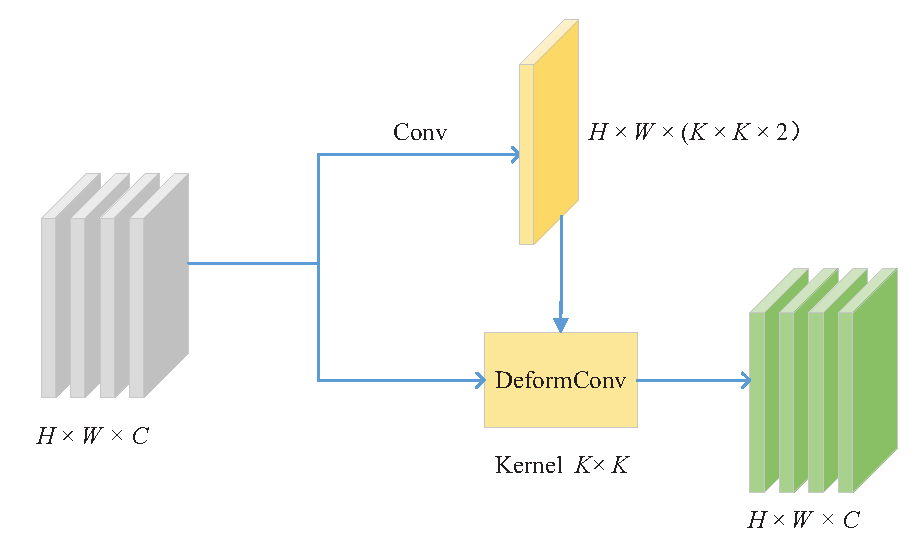
\includegraphics[scale=0.7]{figure/4-3}\caption[如果图题太长,在这里写个短标题只在图索引中出现]{\label{fig:4-3}可形变卷积结构图}
\end{figure}

基于以上描述,图\ref{fig:4-4}展示了本节提出的多分支特征对齐模块的结构。对于从ResNet和FPN主干网络每一层中提取出的特征图,首先通过多分支特征对齐模块自适应地对特征进行重新采样,该模块由三条平行的可形变卷积分支组成,每个分支的卷积核大小为3$\times$3,为了应对遥感图像中目标的多尺度特点,分别使用了扩张率为1、2、3大小的空洞卷积来获取不同大小的感受野,之后将三个分支得到的对齐后的特征拼接在一起,最后再通过一个1$\times$1大小卷积核的结构将通道数调整成与主干网络特征图通道数目相同的输出,将该输出作为新的特征图对感兴趣区域进行特征提取,得到准确的有方向目标的特征表示,进一步提升网络的检测表现。

\begin{figure}
\centering{}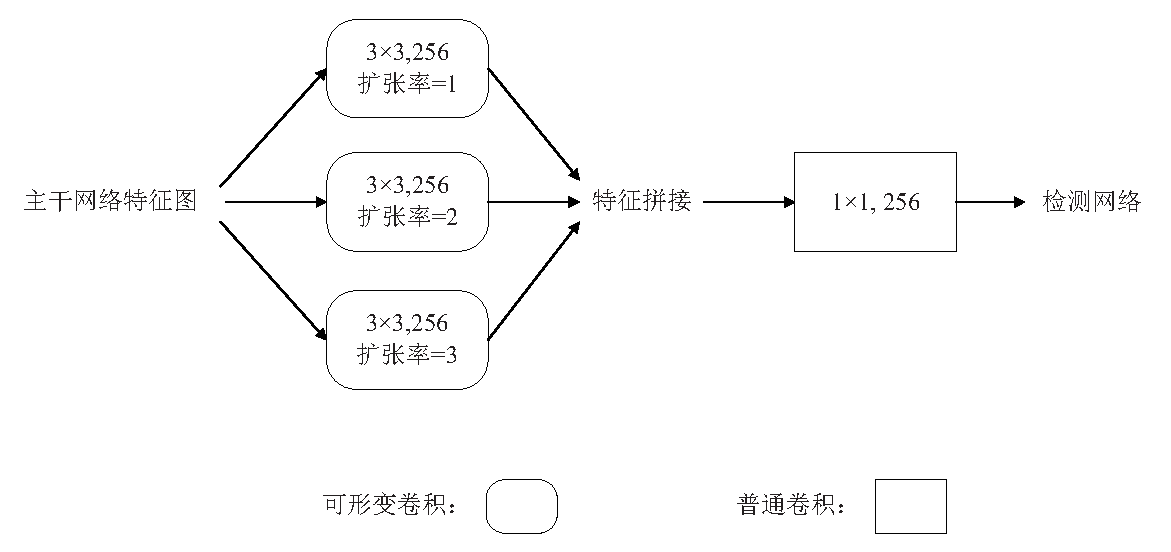
\includegraphics[scale=0.7]{figure/4-4}\caption[如果图题太长,在这里写个短标题只在图索引中出现]{\label{fig:4-4}多分支特征对齐模块总体结构}
\end{figure}

\subsection{基于目标长宽比的角度偏移损失函数}

在传统的基于区域提取的有方向目标检测方法中,为了得到预测的有方向框的中心坐标和尺寸,一般不直接在回归网络对坐标和尺寸大下进行直接预测,而是将标注的有方向框和RPN网络生成的感兴趣区域之间的偏移量作为预测,这样的做法一来可以得到更稳定的损失函数,二来可以加快模型的收敛。在回归分支,感兴趣区域不参与模型的训练过程,只在计算与标注框之间的偏移量编码以及对预测偏移量解码得到最后的输出结果用到,以第一级检测网络为例,对于每一个标注的有方向框($x_g$, $y_g$, $w_g$, $h_g$, $\theta_g$),通过计算与RPN生成的感兴趣区域之间的IoU确定得到对应的作为正样本的感兴趣区域($x_a$, $y_a$ ,$w_a$, $h_a$, 0°),0°表示为水平的感兴趣区域,此阶段的偏移量编码为

\begin{equation}
\begin{aligned}
  &t_x=(x_g-x_a)/w_a,t_y=(y_g-y_a)/h_a \\
  &t_w=\log(w_g/w_a),t_h=\log(h_g/h_a),t_{\theta}=\theta_g-\theta_a
\end{aligned}
\end{equation}
其中$t_x$,$t_y$,$t_w$,$t_h$,$t_\theta$分别为回归分支需要预测的中心点位置,长,宽和角度的偏移量,假定最后得到的预测框为($x_p$, $y_p$, $w_p$, $h_p$, $\theta_p$),则解码得到的回归分支的偏移量输出为

\begin{equation}
\begin{aligned}
  &t_x^{'}=(x_p-x_a)/w_a,t_y=(y_p-y_a)/h_a \\
  &t_w^{'}=\log(w_p/w_a),t_h=\log(h_p/h_a),t_{\theta}=\theta_p-\theta_a
\end{aligned}
\end{equation}
为了可以更加稳定地进行训练,一般来说回归网络的损失函数都是使用Smooth-L1函数,该函数的定义为

\begin{equation}
  L_{SmoothL1loss}=\left\{
    \begin{aligned}
    &0.5(t-t^{'})^2 \qquad if|t-t^{'}|<1 \\
    &|t-t^{'}|-0.5 \qquad otherwise
    \end{aligned}
    \right.
\end{equation}
其中\emph{t}和$t^{'}$分别为真实的偏移量和模型预测的偏移量。然而在使用上述Smmoth-L1损失函数进行有方向目标检测方法的实验中,存在了这样的一个问题:由于不同长宽比目标对于角度偏移的敏感性不一致,导致在对训练好的模型进行测试时小长宽比目标的检测精度要好于大长宽比的目标。图\ref{fig:4-5}展示了不同长宽比目标之间发生的不平衡现象,黄色的框表示的是标注的有方向框,蓝色的框表示的模型最后输出的预测框,红色的框表示的是两个框之间的交集区域,图中对应的黄色框和蓝色框之间有着相同的中心点,长和宽,唯一不同的地方在于角度值,并且图\ref{fig:4-5} (a)和图\ref{fig:4-5} (a)中的两个框之间角度的偏移量也是一样的。在这样的情况下,通过Smooth-L1损失函数计算得到的训练损失是一样的,但是图\ref{fig:4-5} (a)和图\ref{fig:4-5} (b)之间的IoU值相差却极大,很大程度上影响到了最终的检测表现,图\ref{fig:4-5} (a)中的小长宽比的目标有更高的IoU值,在测试阶段该预测框可以被很好的检测到,而图\ref{fig:4-5} (b)中的大长宽比的目标的IoU值过小导致在测试阶段该预测框会被过滤掉,对于此类目标得不到最终的预测结果,影响了目标的检测精度。

\begin{figure}
\centering{}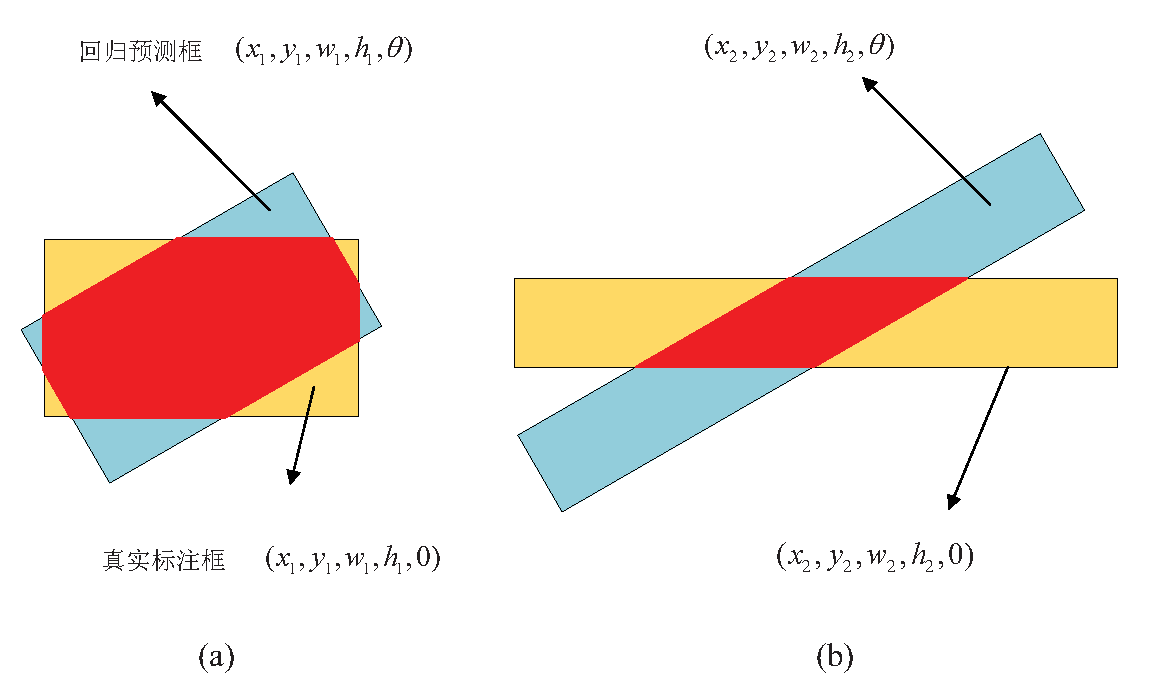
\includegraphics[scale=0.7]{figure/4-5}\caption[如果图题太长,在这里写个短标题只在图索引中出现]{\label{fig:4-5}不同长宽比目标对角度偏移的敏感差异:(a)长宽比为2:1的目标;(b)长宽比为7:1的目标}
\end{figure}

为了解决上述的问题,依据大长宽比目标对角度偏移更加敏感的特点,本章提出了一种基于目标长宽比的损失函数,旨在训练阶段让模型更加关注大长宽比目标的角度偏移量的学习,所以在原有的损失函数的基础上添加了额外的对于角度偏移的惩罚项,最终的损失函数定义如下:

\begin{equation}
  L_{reg}=L_{SmoothL1loss}+|t_\theta-t_\theta^{'}|*(\ln{r}-0.5)
\end{equation}
其中\emph{r}(\emph{r}$\geq$1)表示的是目标的长宽比值,我们观察到对于长宽比特别小的目标(\emph{r}接近于1),只要中心点位置、长和宽的预测准确,角度偏移的准确程度对于最终的检测结果并没有那么重要。因为对于长和宽近乎相等的目标来说,即使有一些角度偏移不会很大影响到最后的IoU值,该目标同样可以在测试阶段被很好的检测到,结果没有受到影响,所以在惩罚项的设计里设定了一个0.5的阈值来确定长宽比值的临界条件,对于长宽比小于该阈值的目标,降低了模型对于其角度偏移量预测的关注度,让模型更加关注于其他偏移量的预测,而对于长宽比大于该阈值的目标,在训练阶段让模型更加关注对于其角度偏移量的学习。

由于遥感图像中的目标长宽比值跨度极大,数据集中的一些目标的长宽比最大可以达到30:1,为了平衡网络对于不同长宽比目标的检测精度,将上述的损失函数应用到了之前提出的两级检测网络的两个回归分支当中。除此之外,分类分支采用的损失函数为常见的交叉熵损失函数。基于此,本章提出的网络结构的总体损失函数定义如下:

\begin{equation}
  L=\frac{1}{N_1}(\sum_{n=1}^{N_1}L_{cls}+s_n^{'}L_{reg})+\frac{1}{N_2}(\sum_{n=1}^{N_2}L_{cls}+s_n^{'}L_{reg})
\end{equation}
$N_1$和$N_2$分别表示两级检测网络中的判定为正样本的感兴趣区域的数量,$s_n^{'}$是一个二进制值,$s_n^{'}$为0当该感兴趣区域分类为背景区域,$s_n^{'}$为1当该感兴趣区域分类为目标区域,即对于背景区域不需要计算回归分支的损失。

\section{本章小结}

由于遥感图像获取时的特殊视角,待检测目标在图像中具有密集分布并且任意朝向的特点,影响了模型的检测表现。针对这样的问题,本章提出了一种两级级联的多方向目标检测方法,增加了一个额外的检测网络来转换得到能更精确表示有方向目标位置的感兴趣区域,缓解了密集分布导致的直接检测时分类分支得分和回归分支定位精度不一致的问题,同时在该检测网络设计了多方向RoI对齐模块获取不同方向区域的池化特征,并在回归分支结合方向注意力模块自适应地对每个方向上的特征进行选取,最后得到的方向敏感特征对于方向多样的目标的回归更加友好。
设计的基于可形变卷积的多分支特征对齐模块来对特征重新采样,考虑了不同长宽比目标对于角度偏移的敏感差异,设计的基于目标长宽比的角度偏移惩罚损失函数,让模型在训练过程中更加关注大长宽比目标角度偏移的学习。实验结果证明,本章设计的模块显著地提升了遥感图像中一些密集分布和大长宽比目标的检测精度。

可以看出,本章节提出的两极级联的多方向目标检测算法很好地解决了任务书中提出的遥感目标多方向性问题。

\chapter{遥感目标多尺度多层次检测网络研究}


\section{引言}

在将通用目标检测中的两步法方法迁移至遥感目标检测任务中时,会受到来自遥感图像多种特殊性质的影响:其一是遥感图像的尺度特殊性,其往往具有极大的分辨率,但传统检测却只能针对小型尺度图像进行分析,无法直接处理具有特大尺度的遥感图像;其二是待检测遥感目标的类间多尺度特性,由于人类活动和建筑的限制,存在诸多小目标聚集的部分,同时这些目标往往在整幅遥感图像中只占有非常小的尺度,而与此同时却还存在着占用较大像素区域的部分场地型目标,显然一个单一尺度的特征提取网络是无法同时应对同一图像中不同尺度的目标的;其三则是遥感图像中目标的密集性,以车辆目标为例,这一类目标会大量存在于公路路口、停车场等位置,这导致目标相互间隔极小,如果在检测时定位不够精细,非常容易将不属于目标的其他噪声与背景作为输入,影响了网络的泛化性能与定位精度。因此不考虑图像和目标尺度适应性的网络往往难以达到与通用目标检测任务中的接近的检测性能与检测效率,其卷积性能也受到了遥感目标多方向性、密集性的影响而更难以提取出具有强鲁棒性的特征图,而鉴于输入图像所具有的前背景信息的迅速增加,在通用目标检测中使用的网络深度难以完全达到最佳检测效果。因此,在本章中,对通用目标检测网络中难以适应遥感检测任务的场景进行分析,并探讨网络性能受到限制的原因,并最终设计了一种深度级联的遥感目标检测网络,以适应尺度多样性的遥感多目标检测任务,同时还基于遥感图像与遥感目标特点,添加了更为针对多方向性目标的可形变卷积结构,从而实现了对遥感图像具有针对性的目标检测网络设计,进而提升检测精度。

但值得关注的是,虽然网络针对遥感图像的小目标性、密集性和多方向性进行了初步的优化与设计,却尚未利用到遥感图像中的特殊信息。与通用目标检测的图像不同,遥感图像往往会标注地面采样距离GSD,也称地面采样间隔。它是存在于遥感与航拍影像中的一个参数,其值的大小说明了图像中的一个像素点所对应的实际地面距离的大小。在DOTA遥感数据集中,由于遥感图像取自于多个卫星图像源,且同一卫星在不同情况下得到的遥感图像也具有不同的拍摄参数与拍摄高度,因此具有不同的GSD。显然的,当遥感图像分辨率相同时,GSD的差异将导致图像所包含的实际区域的大小不同,如图\ref{F5}图\ref{F6}所示即为不同GSD下的两张图像表现,图\ref{F5}的GSD大小为4.47,分辨率为$4526\times 2708$,图\ref{F6}的GSD大小为0.12,分辨率为$9089\times 6473$,可以明显看出,虽然图\ref{F5}的分辨率尺寸远小于\ref{F6},但由于具有较大的GSD,图\ref{F5}中包含有更大、更密集的区域与目标,且这一差异源自于图像拍摄时的参数设置,难以直接通过常用网络的尺度后处理方式进行规避,这直接导致了在大GSD图像中,目标尺度过小较难以被检测的问题较为严重。因此,针对GSD这一特殊信息,本章设计了一个基于图像纹理复杂度的GSD预测网络,试图通过将GSD引入检测过程中,结合图像超分辨思路,对前述遥感目标检测网络进一步优化,从而获得对极小目标的检测能力及在高GSD图像中目标检测准确率的提升。

\begin{figure}
  \centering
  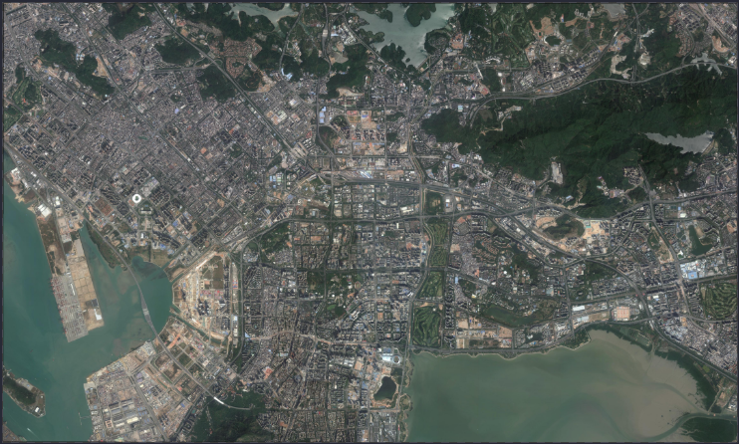
\includegraphics[scale=0.7]{figure/F5}
  \caption{大GSD遥感图像}\label{F5}
\end{figure}

\begin{figure}
  \centering
  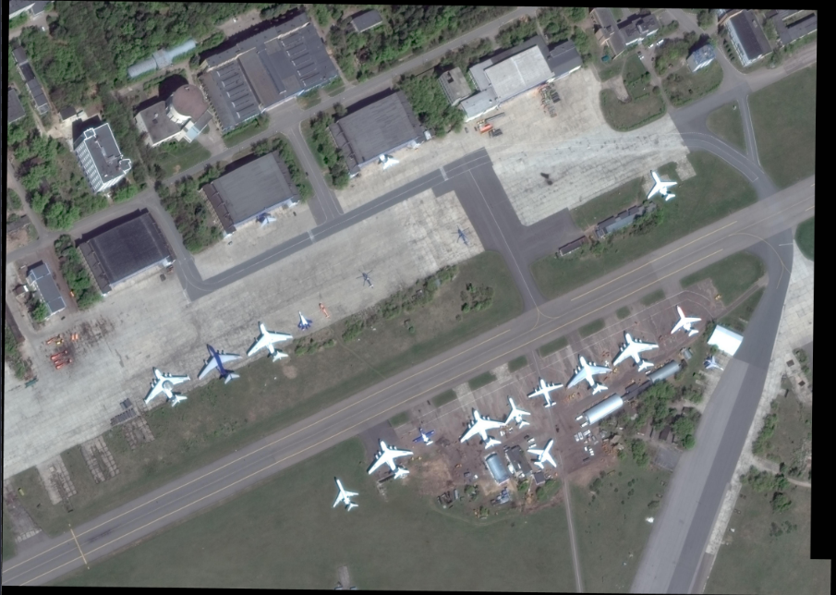
\includegraphics[scale=0.7]{figure/F6}
  \caption{小GSD遥感图像}\label{F6}
\end{figure}

\section{算法设计}
网络整体结构如图\ref{F29}所示,网络主要由三个子模块网络构成,分别是GSD预测网络、超分辨网络及目标检测网络。GSD预测网络可以接收完整的待检测遥感图像,通过对图像纹理复杂度的分析,输出对图像GSD大小的判断结果;而超分辨网络则接收来自GSD预测网络的输出与输入的遥感图像,按照预测结果对图像进行分割和选择性的超分辨,得到若干图像序列;最后,目标检测网络接收前端网络标准化之后的输出作为输入,基于两步法思想执行目标的定位与检测任务,它的输出即为网络的最终输出检测结果。

\begin{figure}
  \centering
  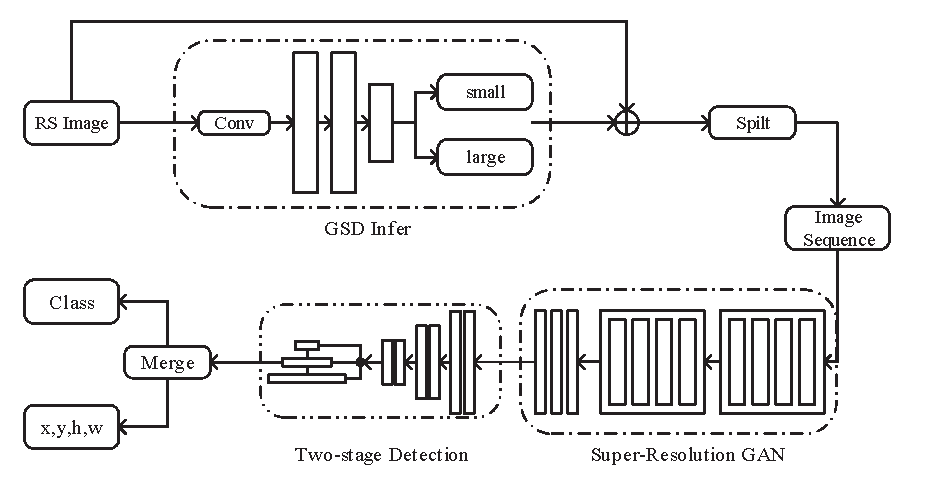
\includegraphics[scale=1]{figure/F29.eps}
  \caption{网络整体结构}\label{F29}
\end{figure}

这里的目标检测网络是我们提出的一种改进的深度级联遥感目标检测网络,其整体框架如图\ref{F9}所示。在Faster-RCNN网络的基础上,改进了特征提取、候选框选取与分类检测的网络结构,使得其对遥感图像具有良好的适应性。网络的具体检测动作流程为:首先将遥感图像进行尺度标准化预处理后,输入backbone网络中进行特征提取,为了确保能够保有图像尽可能多的位置信息与语义信息,使用了一个深度网络ResNet-50作为backbone网络;在进行特征提取时,进一步地利用可形变卷积DCN\cite{21dai2017deformable}进行修正,进而获得更加贴合目标的卷积感受野,减少区域内无关背景的特征噪声干扰;然后将ResNet-50网络中Conv2\_ x、Conv3\_x、Conv4\_x、Conv5\_x的输出层的作为不同尺度的卷积特征图输入FPN结构中,FPN经过自上而下与自底向上的过程后,保留了特征的浅层位置信息与深层语义信息,经由RPN网络进行候选框提取与池化;最终,在检测网络中,构建了深度级联的网络结构,层层级联提高门限值并最终输出检测结果。

\begin{figure}
  \centering
  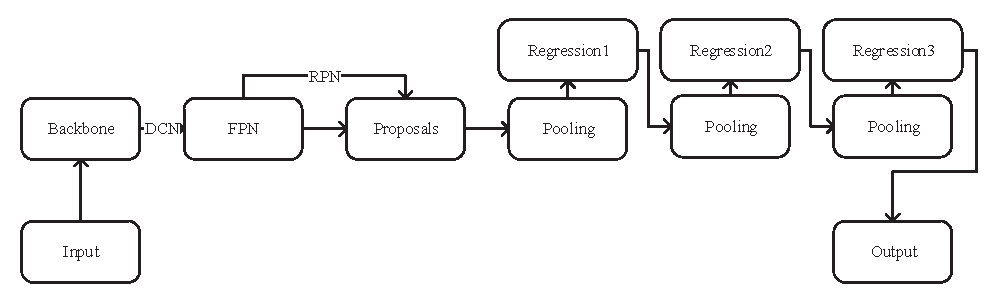
\includegraphics[scale=0.9]{figure/F9.eps}
  \caption{网络整体框架}\label{F9}
\end{figure}

这里我们先介绍改进的深度级联遥感目标检测网络,再介绍融合GSD预测以及超分辨网络进行目标检测。

\subsection{特征金字塔}

FPN特征金字塔结构是一种适用多尺度目标检测的网络结构,在传统目标检测网络中往往使用多层卷积层逐层卷积的结构,其最终输出为一个较小尺度的多通道特征图块,由于通用目标检测中场景往往为局部小区域,同时目标间尺度差异较小,因此这一结构可以取得良好表现。但在遥感图像中,由于遥感图像覆盖了广阔的地面区域,同时其中的待检测目标尺度差异极大,因此,在最终卷积块中,每一像素映射到原图像中都将包含一片较大的区域,显然地,这不利于网络对待检测目标进行精确的定位,更重要的是,在经过多层卷积后,原本尺度极小的部分目标在特征图块中难以保留足够的特征信息,这大大影响了网络对小目标的检测准确率。

\begin{figure}
  \centering
  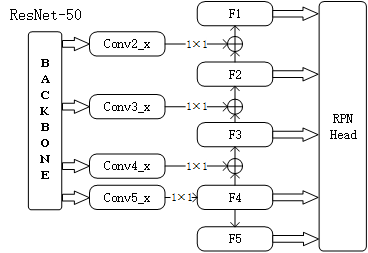
\includegraphics[scale=1]{figure/F10.eps}
  \caption{特征金字塔结构}\label{F10}
\end{figure}

因此,为了能够同时获取到图像中不同尺度目标的特征信息,需要对卷积的输出进行改进,其改进方法是基于不同卷积层次的输出构建特征金字塔FPN网络,其原理在于卷积网络在卷积过程中会随着网络的深入与像素中感受野的增大,逐渐学习到更为抽象的语义特征,对于不同尺度的目标来说,这一过程的最优深度是不一致的,一个较大目标可能需要经过多层的卷积与池化后,才能提炼出核心特征;但对于一个较小目标而言,仅需要较少的卷积便已经得到了高度抽象且准确的特征,如果再进行更深层的卷积池化操作,反而会导致最终特征被过度精炼失去了表征意义。而使用FPN网络可以将单一层级的输出改为多层输出的聚合体,并且同时利用网络不同层之间的信息,来增强检测网络对多种尺度各异的目标的检测能力。图\ref{F10}给出了FPN网络的结构设计,在经过backbone网络ResNet-50的特征提取过程后,取出Conv2\_x,Conv3\_x,Conv4\_x,Conv5\_x层(以下简称C2、C3、C4、C5层),从C2到C5特征图尺度逐渐减小,C2、C3、C4、C5层输出通道数分别为256、512、1024、2048;FPN网络接收这四层输出作为输入,通过一个1×1卷积核建立连接,定义了F1至F4层,其中F1层尺度与C2层相同,以此类推,F4层与C5层尺度一致,需要说明的是,由于1×1卷积核的加入,让F1至F4层通道数被限制为256,F4层由C5层连接得到,而其上层F3则由C4层经由1×1卷积与F4层经由上采样后融合得到,同理F2、F1层;而F5层则是由尺度最小的F4层经由下采样方法得到,一般地,可以使用最大池化或卷积的方式进行,在此网络中使用了最大池化方式得到F5层。就此得到了FPN的五层输出F1至F5,其尺度逐层降低,这五层将分别地送入RPN阶段提取候选框。

FPN的加入,有效保留了遥感图像中的多尺度特征,通过自顶向下的卷积过程提取出多尺度目标特征,随后经由自底向上的融合过程,将底层获取的语义特征与原有层特征融合,在保有高层次语义特征的同时增强了低层次位置信息,使网络获得了对遥感多尺度性的适应能力。


\subsection{可形变卷积}

在遥感目标检测任务中,由于小目标特性与目标密集性的存在,对特征的提取过程受到了极大关注,如何提取到更贴近目标、更鲁棒的特征,且减少其他无关目标与背景的噪声干扰成为切入点。而回到卷积过程中,通用的卷积核设计往往为\emph{n×n}的正矩形,这就意味着在层层深入的卷积中,最终特征图中的一点,其对应的感受野始终保有这一矩形特性,但在遥感图像中,目标往往并不具有类似的规则性,且目标还具有密集多方向的显著特性。因此,为了增强卷积特征提取过程,适应遥感目标的特殊性,将可形变卷积结构加入了特征提取网络中,通过更改卷积核感受野,加入偏移量,增强了特征的鲁棒性与识别的准确率。

\begin{figure}
  \centering
  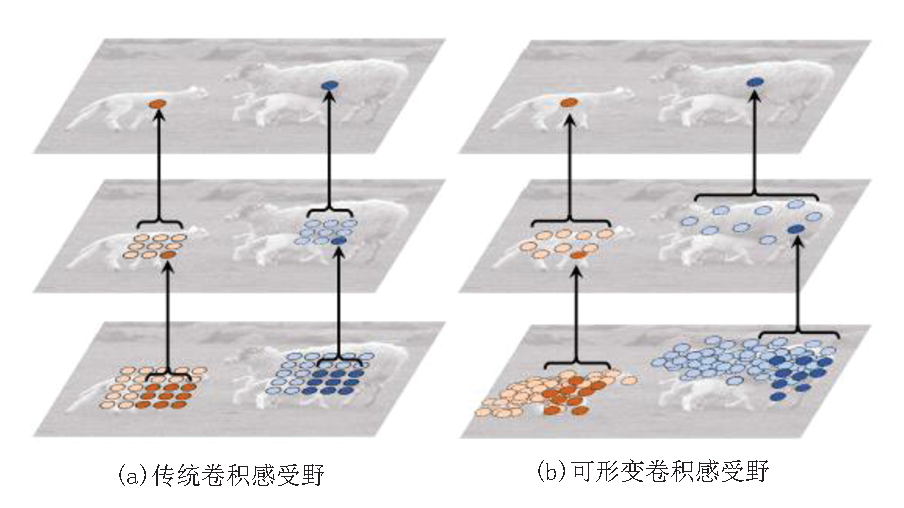
\includegraphics[scale=0.8]{figure/F11.eps}
  \caption{可形变卷积感受野}\label{F11}
\end{figure}

可形变,即卷积核感受野的可形变性,如图\ref{F11}所示,图(a)为传统卷积过程中感受野的逐层映射关系,而(b)为可形变卷积感受野的逐层映射关系。显然的,在可形变卷积过程中,卷积核所选取的卷积区域不再是一个规则的矩形区,而是由若干分散点像素组合而成,在经过训练学习后,可以使得这些点贴近到目标存在前景的不规则区域内。

\begin{figure}
  \centering
  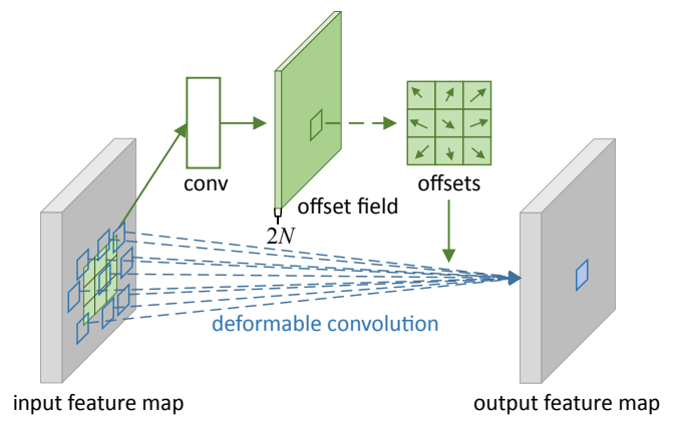
\includegraphics[scale=0.7]{figure/F12}
  \caption{偏移学习网络}\label{F12}
\end{figure}

要达到可形变的卷积效果,需要在卷积时给被卷积图像中的每一像素点施加一个偏移量,而要使得偏移量与目标区域相匹配,则需要利用无监督的方法进行学习,图\ref{F12}给出了这个无监督学习的网络结构。网络的输入为上一层卷积结构的输出特征图块,在进行下一次卷积之前,将其送入一个卷积结构中,与特征提取中的卷积结构不同,这一卷积结构对偏移量敏感,输出的是与输入同等尺度的偏移预测图,当输入的特征图维度为\emph{h×w×N} 时,得到的偏移预测图则为\emph{h×w×2N},其中2\emph{N}代表了对原特征图\emph{N}通道上同位置像素点在原始特征图像中\emph{x}轴、\emph{y}轴上的偏移量(\emph{x\_offset, y\_offset}),在此之后,代入偏移量进行特征提取的卷积过程如式\ref{equ2}所示:

\begin{equation}\label{equ2}
  y(P_{0})=\sum_{P_{n}\in \Re}^{}w(p_{n})\cdot x(p_{0}+p_{n}+\Delta p_{n})
\end{equation}
其中\emph{$\Delta p_{n}$}由式\ref{equ3}计算得到:
\begin{equation}\label{equ3}
  \Delta p_{n}=\sqrt{\emph{x\_offset}^{2}+\emph{y\_offset}^{2}}
\end{equation}
在计算过程中,有两点需要加以限制:

1.	由于偏移量是通过预测网络学习得到,因此其值不为整数,显然,代入偏移量后得到坐标(\emph{x+x\_offset, y+y\_offset}),如图\ref{F13}所示,对该点坐标值上下分别取整,可以得到一个四点矩阵,而小数位置在图像的像素操作中没有实值,因此,需要使用插值法计算出实际得到像素值大小,在本网络中使用双线性插值实现,因此其计算方法可以由式\ref{equ4}表示,展开为式\ref{equ4*},通过周围四个整数像素点的值加权计算得到结果。其中\emph{f(Q)}表示该点的像素值大小;

\begin{figure}
  \centering
  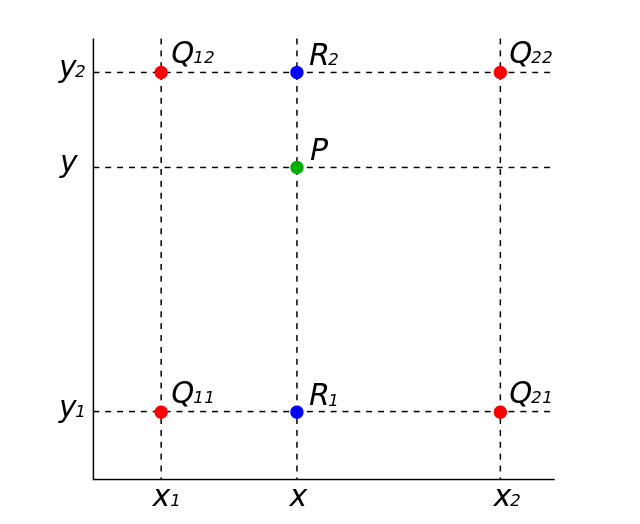
\includegraphics[scale=0.3]{figure/F13}
  \caption{双线性插值}\label{F13}
\end{figure}

\begin{equation}\label{equ4}
  {f}(P)=\begin{bmatrix}
                (x_{2}-x) & (x-x_{1}) \\
              \end{bmatrix}
              \begin{bmatrix}
                f(Q_{11}) & f(Q_{12}) \\
                f(Q_{21}) & f(Q_{22}) \\
              \end{bmatrix}
              \begin{bmatrix}
                (y_{2}-y) & (y-y_{1})
              \end{bmatrix}
\end{equation}

\begin{equation}\label{equ4*}
\begin{split}
  f(P)=&f(Q_{11})(x_{2}-x)(y_{2}-y)+f(Q_{21})(x-x_{1})(y_{2}-y)\\
  & +f(Q_{12})(x_{2}-x)(y-y_{1})+f(Q_{22})(x-x_{1})(y-y_{1})
\end{split}
\end{equation}

2.	其次,当偏移量超出原特征图分辨率尺度范围或为负值时,对应原特征图像上得到的点也是无意义的,因此在预测网络中加入需要加入边界限制,确保其计算结果在特征图尺度之内,是可以计算的且有意义的。

在本网络中,基于对网络中各卷积层尺度及其对应感受野的大小进行分析,结合需要检测的目标其尺度特征在卷积层中的分布确定修改方案。在backbone的ResNet-50的Conv3\_x,Conv4\_x,Conv5\_x层中加入了可形变卷积结构,能够在不占用过多计算资源的同时增强对遥感图像中密集性、多方向性目标的特征提取能力。
\subsection{级联网络}

级联网络的思路最早在Cascade RCNN\cite{35cai2018cascade}中被提出,其关注的是网络中设置的IoU门限值对检测结果的影响。在常见的两步法目标检测方法中,RPN网络通过多比例与多尺度的锚点anchor来得到候选框,在遍历图像时,会在同一像素处置生成多个形状的检测框,为了尽量避免其中重复检测框问题的出现,在检测网络中往往会设置IoU门限对候选框进行筛选,IoU的计算方式由式\ref{equ5}给出,其中A、B表示独立的两个检测框,显然当两个检测框越接近时,它们交集越大、并集越小,IoU计算值也越大;反之当两个检测框非常疏远时,IoU计算值会趋近于0,IoU值在某种程度上表征了两个检测框重合度的大小。

\begin{equation}\label{equ5}
  IOU=\frac{A\bigcap B}{A\bigcup B}
\end{equation}

因此,在网络训练过程中,通过更改IoU门限大小,可以人为地影响网络学习效果。在IoU门限值较低时,大量与真实检测框相关性较低的检测框作为正样本被保留,导致检测结果中出现无关背景与其他噪声;当IoU门限升高时,只有和真实框非常相近的检测框得以保留,此时网络能学习到精确的目标信息,但由于检测产生的正样本数量急剧减少,网络存在过拟合的风险。 对于一个目标检测任务而言,检测框预测与真实值越接近,在检测结果上体现为网络对目标的定位能力越强,可以更准确地预测出目标位置。因此级联的思想也就有了立足之地,其核心在于,当候选框经过检测器后,其输出预测框与目标真实标注(Ground Truth, GT)的IoU会增大,可以得到一个具有良好数据分布的结果,那么只要将输出再次作为输入,此时更为精确的检测框可以导致普遍的IoU提升,进而避免了在IoU过高时,检测正样本过少导致的过拟合问题。因此当使用多个检测网络级联时,通过使用前一阶段的检测结果去训练下一阶段的检测器,可以人为地提升IoU门限而不产生过拟合问题,同时也提高了网络的检测能力。在本章提出的网络中,便以此思路设计了三级级联的检测网络S0、S1、S2,对其IoU门限值设置分别为0.5、0.6、0.7逐层递增,将S0网络检测输出框的仍含有较多噪声的结果送往S1中继续训练,并同样地取输出送往S2进行检测,最终将S2输出作为网络最终输出,这一结构提升了检测网络的学习能力,给遥感图像中密集目标与小目标的检测带来助益。

\subsection{GSD预测网络}

在计算机视觉领域,图像复杂度(Image Complexity)可以从多个维度进行评估,如色彩复杂度(Color Complexity)、纹理复杂度(Texture Complexity)与形状复杂度(Shape Complexity)\cite{31周兵2018图像复杂度研究综述}。在遥感图像中,GSD的大小决定了像素所代表实际地面距离,可以推断出,GSD间接地决定了在遥感图像中一个单位像素块所包含的实际区域大小,显然地,GSD越大,对于同样的地理区域而言,图像所涵盖的区域内建筑、目标、背景环境就越复杂,而这一复杂性可以通过图像的纹理复杂度得以体现,因此一种基于遥感图像纹理复杂度的GSD预测网络应运而生,其整体算法流程如图\ref{F17}所示,主要由预处理、纹理提取和距离估计三部分构成。

\begin{figure}
  \centering
  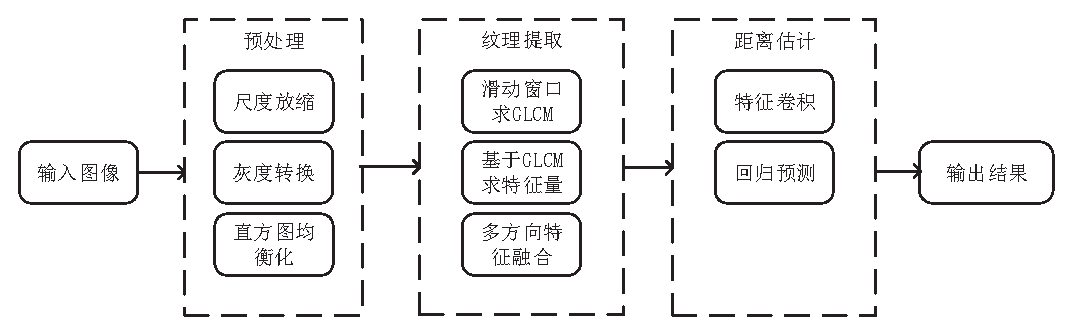
\includegraphics[scale=0.8]{figure/F17.eps}
  \caption{GSD预测网络}\label{F17}
\end{figure}

\subsubsection{预处理}

预处理环节在提取遥感图像纹理特征之前先对输入图像进行一定的处理,使其能够符合后续处理的尺度、色彩要求,避免结构性误差的引入。一般地,基于输入图像特性,从以下几个方向进行预处理:

1.尺度放缩。遥感图像往往具有常规意义上的过大分辨率,而在进行图像的纹理特征提取与GSD预测时,需要确保输入的完整性,防止因局部平滑导致的误判和错漏。因此对图像的尺度进行放缩是很有必要的,这样就能利用图像的尺度不变性特征,在计算量较小的情况下进行纹理提取工作,降低了不必要的资源消耗,提升了网络整体运算效率;

2.灰度转换。多通道图像会使得图像的纹理提取工作更为复杂,但与此同时却不能显著增强提取出的纹理特性,因此基于优化网络结构、提升网络计算效率的目标,可以将输入的彩色图像以一定方式转化为灰度图像,具体计算方式如式\ref{equ6}所示,其中R、G、B分别代表图像RGB通道对应像素值,该转换方式是由计算机图像处理及人眼视觉感知的通用准则规定而成,以认知心理学对于RGB图像色彩的研究为基础,可以最大程度的确保灰度图像与原图像在视觉感知、图像处理中的一致性。
\begin{equation}\label{equ6}
  Y=0.299R+0.587G+0.114B
\end{equation}

3.灰度直方图均衡化。这是一种传统的灰度图像处理方法,其目标是使得图像灰度分布更为均衡地分布在整个灰度域之上,使图像的亮暗都更加明显,增强了对比度。在图\ref{F18}中,图(a)为原灰度图像,图(b)为经过直方图均衡化之后的灰度图像,相比于原图,均衡化使得图像中明度对比度得到增强,图像细节进一步凸显,纹理更加清晰,便于后续处理。

\begin{figure}
  \centering
  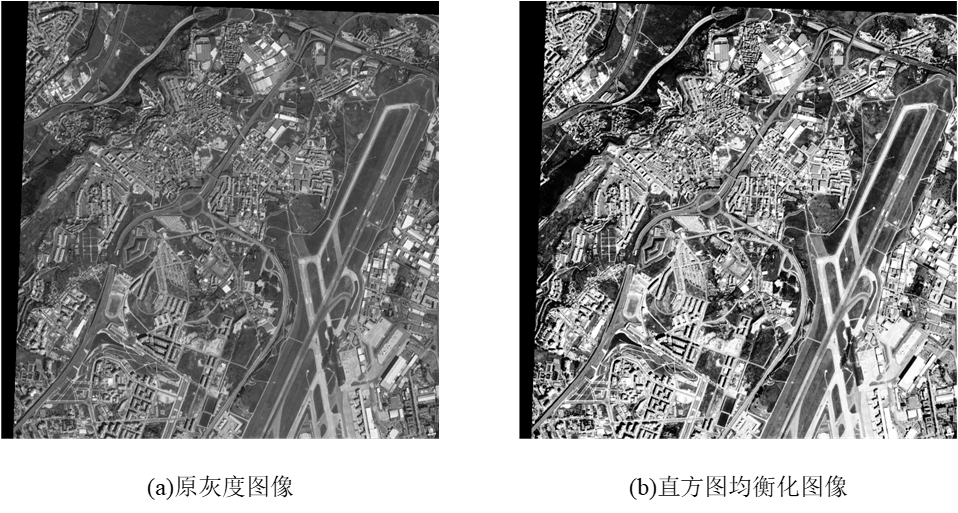
\includegraphics[scale=0.5]{figure/F18}
  \caption{直方图均衡化}\label{F18}
\end{figure}

\subsubsection{纹理提取}

在图像分析领域,常常通过计算灰度共生矩阵及其特征值(Gray-Level Co-occurrence Matrix, GLCM)\cite{34haralick1973textural}来对图像的纹理复杂度进行评估。在文章中,灰度共生矩阵被定义如下:设一灰度图像具有\emph{N}个灰度值,那么计算得到的灰度共生矩阵的大小就为\emph{N×N}阶,规定一个像素对偏移量为δ,它意味着计算时需要不断地在图像中按角度θ去遍历距离为δ的像素对\emph{a}、\emph{b},可以得到其灰度值对(\emph{a$_{k}, b_{k}$}),随后将具有相同灰度值对的像素对数量累加,对应着灰度共生矩阵中(\emph{a$_{k}, b_{k}$})的元素\emph{G}(\emph{a$_{k}, b_{k}$})的值。当遍历完整个图像之后,就得到了该图像对应的灰度共生矩阵G。

\begin{figure}
  \centering
  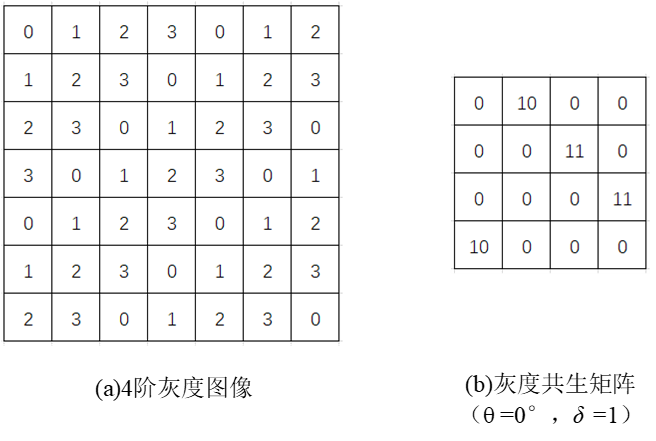
\includegraphics[scale=0.6]{figure/F19}
  \caption{灰度图与灰度共生矩阵}\label{F19}
\end{figure}

如图\ref{F19}所示为一幅具有4阶灰度级的灰度图像及以水平方向进行遍历得到的灰度共生矩阵,显然地,灰度共生矩阵是基于像素对灰度值的统计量,它记录了在图像当中不同灰度匹配模式的出现次数,而δ则代表了该灰度共生矩阵对于灰度纹理精细级别的敏感度,当δ越小时,像素对间距较小,则检测的纹理较细致,反之则纹理越粗糙。

进一步的,当使用不同的距离δ与遍历角度θ时,可以得到设置不同方向与不同距离时的灰度共生矩阵如图\ref{F20}所示。这体现了灰度共生矩阵对于纹理方向的敏感性。一般地,为使提取到的纹理特征具有一定的旋转不变性,会特别地使用0°、45°、90°、135°这四个角度进行计算,距离则由图像中主要纹理的粗糙程度来定义。
\begin{figure}
  \centering
  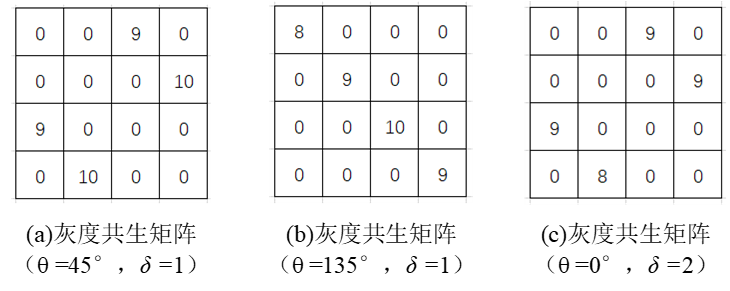
\includegraphics[scale=0.5]{figure/F20}
  \caption{不同条件下的灰度共生矩阵}\label{F20}
\end{figure}

灰度共生矩阵具有着图像的纹理统计信息,但就作为图像纹理特征而言,其鲁棒性尚不能满足要求,不够直观也是一个巨大的不足,研究者们难以直接利用灰度共生矩阵进行比较和分析。因此,在提出灰度共生矩阵的同时,Haralick团队也给定了14个用于纹理分析的计算统计量,也即纹理描述子,分别为:二阶矩、熵、对比度、均匀性、相关性、方差、和平均、和方差、和熵、差方差、差平均、差熵,同质性及最大相关系数,但彼时他并未给出这些统计量的有效性与相关性结论。随后,Barald\cite{39baraldi1995investigation}等人经由研究计算论证,说明在Haralick给出的14个统计量中,其中4个统计量之间不相关性最强,对于遥感图像具有较好的特征表现能力。分别是:

1.	二阶矩(Angular Second Monment, ASM),也被称作能量,其计算方法由式\ref{equ8}给出,其中\emph{P}(\emph{i, j})为灰度共生矩阵中位于(\emph{i, j})处的元素归一化概率。ASM对灰度共生矩阵内值的和大小敏感,当图像纹理分布均匀、纹理粗细程度接近时,ASM可以获得较大值;
\begin{equation}\label{equ8}
  Asm=\sum_{i}^{}\sum_{j}^{}P(i,j)^{2}
\end{equation}

2.	熵(Entropy, ENT),在物理学领域中,熵被用来描述一个系统的混乱程度。在此处,其计算方法由式\ref{equ9}给出,它具有类似的描述功能,可以用于表现图像中纹理的复杂程度或分布的非均匀程度,当熵值越大时,意味着图像中纹理随机性较强、分布较为复杂,显然地,对于一张纯色图像,其熵值为0;
\begin{equation}\label{equ9}
  Ent=\sum_{i}^{}\sum_{j}^{}P(i,j)logP(i,j)
\end{equation}

3.	同质性(Homogeneity, HOM),也被称为逆方差。其计算方法由式\ref{equ10}给出,正如其名,同质性关注的是图像中局部区域的纹理变化情况,当不同区域间的图像纹理变化较为缓慢平滑时,其值较大,反之较小的同质性意味着不同区域间纹理变化剧烈;
\begin{equation}\label{equ10}
  Hom=\sum_{i}^{}\sum_{j}^{}P(i,j)^{2}/[1+(i-j)^{2}]
\end{equation}

4.	非相似性(Dissimilarity, DIS),这是一类用于度量图像局部或整体区域内灰度差异区分度的统计量,其计算方法由式\ref{equ11}给出,通过公式可以发现,DIS与灰度间的度量具有线性关系。
\begin{equation}\label{equ11}
  Dis=\sum_{i}^{}\sum_{j}^{}P(i,j)|i-j|
\end{equation}

除此之处,基于对图像信息的提取需求,还有另外几类较为直观的统计量也常常被用于计算之中,如均值、对比度及相关性等,其中均值表征了图像中灰度的整体或局部明暗度,当图像中出现规则、易于描述的纹理时,均值将具有较大值;对比度是对图像中局部像素与其周围像素的灰度差距的度量,灰度共生矩阵对比度与图像对比度表征类似,越大对比度的图像说明在图像中纹理越清晰,边界较明显\cite{40高程程2010基于灰度共生矩阵的纹理特征提取};相关性则具有方向敏感性,其与计算时遍历图像的方向有关,它揭示了在图像中沿着某一特定方向上灰度纹理的延伸长度,与非相似性DIS类似,它也是一个灰度关系的线性度量统计量。

需要更进一步指出的是,上述的所有统计量都是标量形式,在一些简易灰度图像处理方法中,往往将这类统计量进行联合,构建一个多维矢量对图像进行纹理的表征,称之为特征矢量,然后利用特征矢量代入计算之中执行相似性对比、分类等任务。但在遥感图像中,这一方法存在若干不足之处,其一是遥感影像更为复杂,由于其覆盖广阔,影像中会存在多种地块与丰富的目标,单一统计量在复杂图像中显得较为乏力,区分维度不够,无法表征出图像局部纹理特征,如水域与城市共存时,即无法体现出水域的统计特性,也难以表征城市建筑的纹理特征,使得不同地域、不同纹理下的遥感图像在特征矢量中差异性较小、边界不易区分,严重降低了遥感图像纹理特征的表征能力与可识别性。因此,借由卷积神经网络的启发,在本设计中,将滑动窗口思想应用于灰度共生矩阵的计算当中,使用了基于局部灰度共生矩阵的特征图表征方法,该算法主要有以下步骤构成:

1.	设置一个7×7的滑动窗口,padding为3,步长为1,窗口起始位于图像左上角;

2.	针对滑动窗口中的7×7图像区域以前述定义的计算方法进行统计,得到对应的局部图像灰度共生矩阵;

3.	计算得到的局部灰度共生矩阵中均值、方差、同质性、对比度、非相似性、熵、能量、相关性和自相关等一系列统计量,分别输出作为该滑动窗口的输出,其输出形式为多维度矢量;

4.	将滑动窗口按照既定的步长,以从左至右,自上而下的轨迹对遥感图像进行遍历,每次移动后重复第2、3步骤得到输出;

5.	待滑动窗口遍历结束,将期间的所有输出按统计量类别组合,可以得到多幅特征图像,图像与原输入图像具有相同的分辨率,但仅仅表征了图像的灰度共生矩阵在某一特定统计量下的表现;

6.	重复1至5的步骤,但在计算灰度共生矩阵时,分别使用0°、45°、90°、135°对纹理进行统计;

7.	将同一图像中同一纹理统计量在不同计算角度下的特征图以平均加权的方式进行加和,得到最后的特征图像,由于本网络中设计了9类统计量表征纹理特性,因此得到H×W×9维度的纹理特征图像,其中H、W为输入图像的高与宽。
\begin{figure}
  \centering
  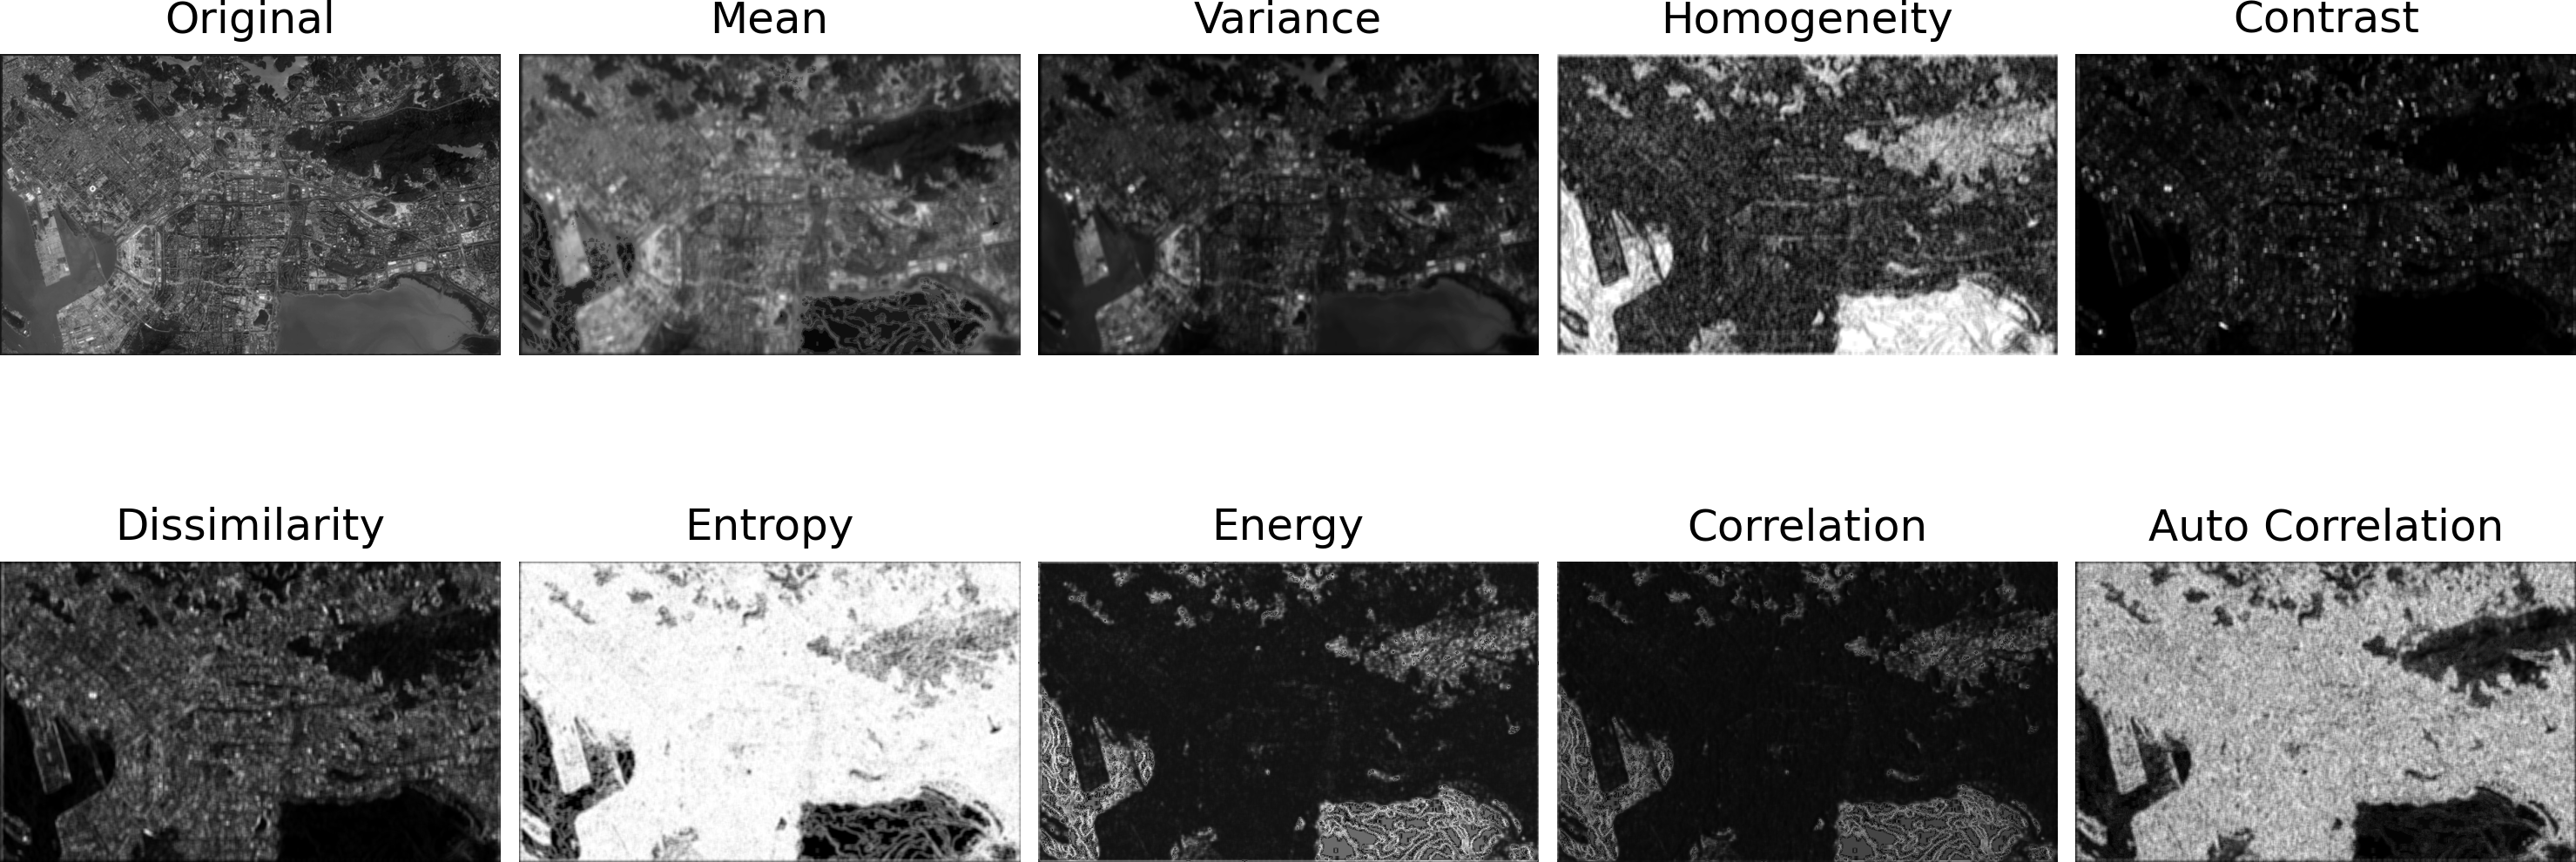
\includegraphics[scale=0.5]{figure/F21}
  \caption{大GSD图像GLCM}\label{F21}
\end{figure}

\begin{figure}
  \centering
  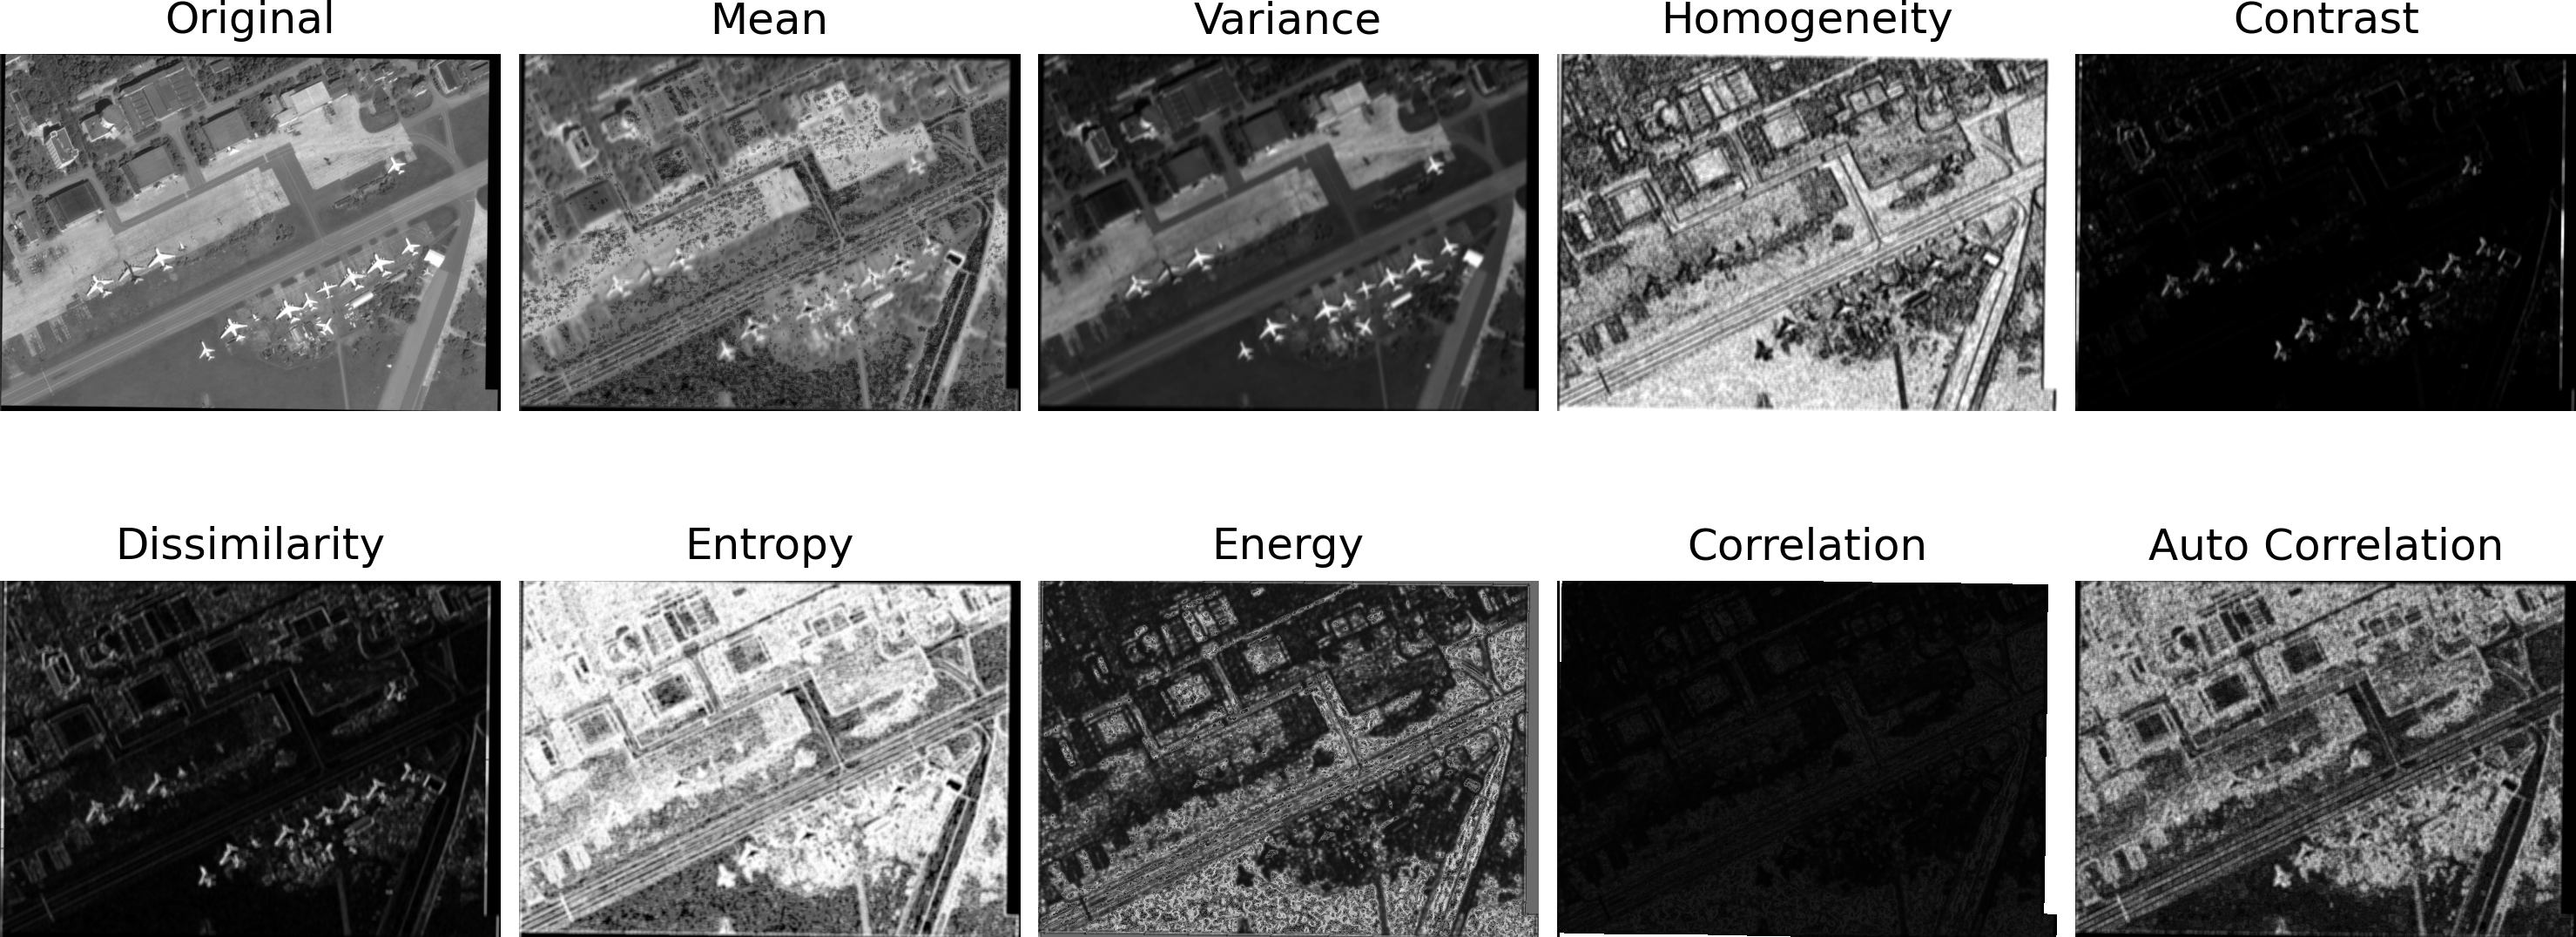
\includegraphics[scale=0.5]{figure/F22}
  \caption{小GSD图像GLCM}\label{F22}
\end{figure}
至此,获得了一幅输入遥感图像的纹理特征图,它同时具有着局部特征与整体特征的信息,且在多个方向上都具有一定的纹理敏感性,最大程度地提取了图像中由不同地块、不同目标和不同区域所产生的纹理特征,为评估图像复杂度提供了坚实依据,为后续GSD预测提供了可靠鲁棒的输入。图像\ref{F21}和图\ref{F22}给出了对图像\ref{F5}和图\ref{F6}的纹理特征提取图结果。



\subsubsection{距离估计}

距离估计网络的设计目标是通过学习图像的复杂度,尤其是纹理复杂度的信息,合理推测出图像拍摄时的GSD参数状态。各领域研究者也曾提出过相应的方法来利用灰度共生矩阵信息,如Wed等人便利用GLCM与K-means聚类算法相结合,试图以无监督的方式对医学影像中的病症点进行分析\cite{41oleiwi2018alzheimer};还有Naveena等人则将GLCM与SVM分类器相结合,在树叶分类问题中取得了显著表现\cite{42vidyashanakara2018leaf}。然而,在遥感图像领域,这类方法效果却并不尽如人意,这是因为遥感图像具有较大分辨率与较为丰富的图像内容,在简单线性分类方法中会带来过高维的复杂度,占用过多计算资源。
\begin{figure}
  \centering
  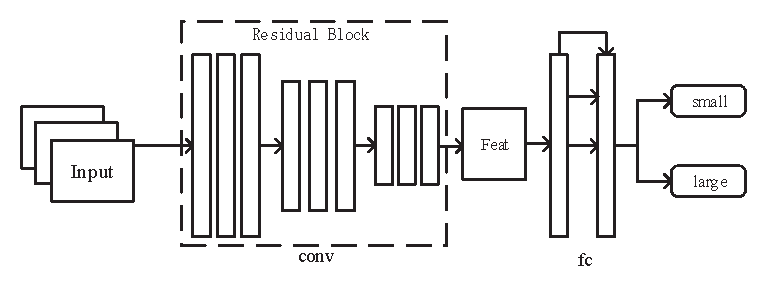
\includegraphics[scale=1.2]{figure/F23.eps}
  \caption{预测网络结构}\label{F23}
\end{figure}

因此,基于对输入图像内容的复杂性进行估计的需求出发,本章节中提出了一种使用深度卷积网络提取特征并回归分类预测遥感图像GSD的方法。网络结构以ResNet-50为基础进行修改,因为其深度能够满足特征提取与学习的需求。具体结构如图\ref{F23}所示,输入图像为前述计算所得到的纹理特征图像块,在输入网络前,为满足网络卷积输入条件,需要先将其尺度调整为224×224,随后设计了多个残差卷积块,每个残差块由1×1和3×3的多个卷积核叠加而成,最终展平后得到1×1×4096维的特征图像,在池化层利用平均池化方式进行降维后,直接与全连接层FC1相连,FC1具有2048个神经元,它的输出经由密集全连接输入全连接层FC2的512个神经元,最终汇集为两类输出,完成回归分类并输出标签。基于本次使用数据集DOTA中的图像GSD实验特性,当GSD较小时,检测网络对目标仍能具有较好的适应性,而当GSD过大时,网络无法识别出其中的极小目标,因此在GSD预测输出中将图像分类为正常GSD尺度与过大GSD尺度两类。网络使用Adam优化器进行反向梯度传播,损失函数为交叉熵损失,如式\ref{equ12}所示,在本网络设计中\emph{N}为2,\emph{L$_{i}$}为单一类别的交叉熵损失 。

\begin{equation}\label{equ12}
  L=\frac{1}{N}\sum_{i}^{}L_{i}=\frac{1}{N}\sum_{i}^{}-\sum_{c=1}^{M}y_{ic}log(p_{ic})
\end{equation}

在进行网络设计时,曾经存在着另一方案的设计,即将GSD准确值或近似值作为回归的预测目标。但经过实验证明,这一方案存在两个不足之处:其一是GSD与图像复杂度特征间为非线性关系且不具有强烈相关性,对于遥感图像这类具有较高复杂度的图像而言,要将其与单一精确数值进行关联是非常困难的;其二是由于后续需要使用超分辨等图像尺度变换操作,为确保其输出效果准确,对于图像输入尺度与放缩比例具有严格要求,无法直接利用预测出的精确值进行操作,防止在超分辨过程中引入不必要噪声干扰检测结果。因此,综上两点所述,使用分类预测方案,对遥感图像的GSD值进行预测是一个能在检测效率、识别准确率及资源利用率上达到平衡的方法,具备一定的优势。


\subsection{图像超分辨}

前述对图像的分析与预测工作,其最终目的都在于提取遥感图像的GSD信息,并将其引入网络之中。在本节中,正是出于对GSD信息的利用方法进行思考,设计了一个遥感图像超分辨网络,其逻辑意义在于:基于图像\ref{F5}和\ref{F6}的分析可以发现,当在不同GSD图像中取同样大小像素块时,对于图像中的同类目标,其体现在像素尺度之上的差距正是两图像GSD的比值,此外,研究者们的一致认知是,对于现有的遥感目标检测网络而言,由于其训练时大部分目标都分布于正常GSD尺度之下,网络学习到了这一尺度敏感性,所以难点之一便是在大GSD图像中出现的极小目标,其尺度比正常尺度下的同类目标缩小了数倍,故难以被网络检出。因此,一个利用GSD信息的方法便自然地产生,即将大GSD图像通过某种方式进行放大,人为地调整图像GSD的大小,使之接近正常GSD图像,从而增大对大GSD图像中极小目标的检测能力。

传统的图像放大方法主要有插值类方法,其主要原理是参考原低分辨率图像中的相邻像素值,对得到的高分辨率图像中空白像素进行填充,根据插值内核处理方法不同可以分为线性插值方法如最邻近插值、双线性插值和三线性插值等方法,和非线性插值方法如基于边缘信息的插值方法、基于小波系数的插值方法等\cite{43钟宝江2016图像插值技术综述};而超分辨网络方法则是基于神经网络学习的方法,其所利用来超分辨的信息并不局限于单一输入图像,而是基于多幅图像的学习结果来估计目标高分辨图像的像素值,超分辨网络得到的图像像素与原低分辨图像间并不存在严格的位置映射关系,严格来说,新图像中每一个像素都是重新计算得到,不会保留原有图像中像素的所有信息。传统方法较为简单,运算速度快,且能适应更为灵活的图像放大倍率,但它只能基于输入图像中所具有的像素信息进行放大,对于大型图像或较为复杂的图像,其输出图像在视觉效果及噪声检测指标上都存在不足;而超分辨类方法则能适应复杂图像的放大任务,但需要使用大量已知标定数据进行预先训练,且计算时间相对较长,由于网络结构的限制,对放大倍数和输入尺度存在限制,只有在预设倍数和尺度下工作时才能发挥网络的最佳性能。综合这两类方法的优劣,在本网络中,针对遥感图像显然使用超分辨网络更为合适,而在之后的实验中也证明了这一点。

\begin{figure}
  \centering
  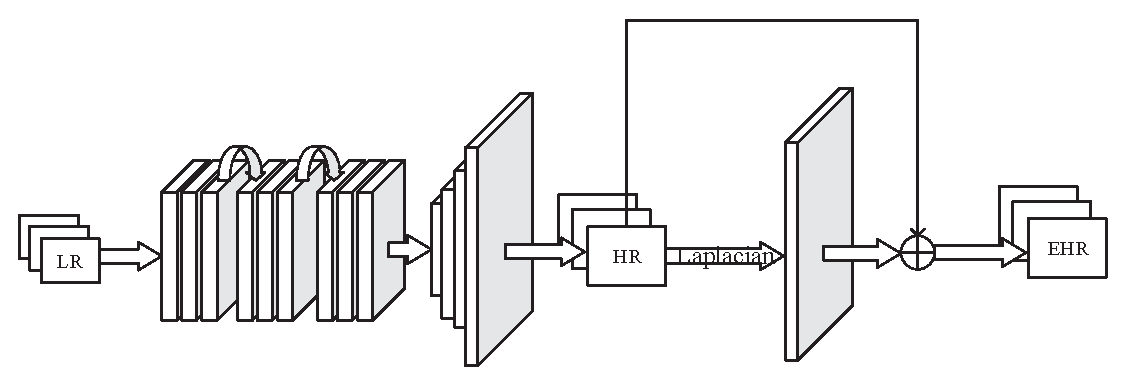
\includegraphics[scale=0.6]{figure/F24.eps}
  \caption{超分辨网络结构}\label{F24}
\end{figure}
本章所使用网络结构为对抗生成网络(Generative Adversarial Network, GAN),最初的GAN结构是由Goodfellow\cite{44goodfellow2014generative}提出,GAN网络正如其名,具有“生成器”与“判别器”之间的对抗过程,生成器以某一规则不断生成与真实样本相似的样本或分布,如音频样本、图像样本和文本样本等,而判别器则被设计成为具有类似特征提取与识别功能的网络,它需要将生成样本与真实样本进行区分,这两部分互相拮抗,通过构建相关联的损失函数进行相互优化。而在超分辨任务中,生成器的任务便是基于原始低分辨率图像(Low Resolution, LR)生成高分辨率图像(High Resolution, HR),经由判别器与原高分辨率图像对比得到误差,不断优化生成图像质量,从而实现图像超分辨。如图\ref{F24}所示即为本网络中使用的超分辨网络的示意结构,首先以超分辨网络SRGAN\cite{45ledig2017photo}的生成器结构为基础,考虑到遥感图像的特殊性,泛用的超分辨方法很容易导致输出的图像中出现地面细节部分的模糊,严重影响到遥感目标的检测与定位,因此在后端加入一个边缘提取网络对得到的高分辨率图像进一步增强,并把增强后具有边缘信息的边缘增强高分辨图像作为网络的最终输出,其具体的操作步骤如下所述:

1.	首先将需要超分辨遥感图像进行尺度裁剪至预定大小的多张图像,获得尺度一致的输入低分辨率图像LR;

2.	利用多个残差块构建生成器网络,每个残差块结构如图\ref{F25}所示,包含有两个3×3×64的卷积层,其步长为1,在卷积层之后加入批归一化处理(Batch Normalization, BN)与PReLU(Parametric Rectified Linear Unit)作为激活函数;由多个残差块进行连接,在此过程中特征特图块的通道数逐渐增长,从广义上看便是逐渐学习到了高分辨图像所缺失的内容,最后连接3×3×256卷积层并进行维度变换,得到3通道放大尺度图像,达到了对图像进行上采样的目的,并输出高分辨率图像HR;
\begin{figure}
  \centering
  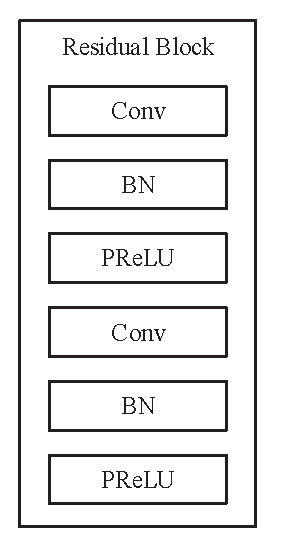
\includegraphics[scale=0.8]{figure/F25.eps}
  \caption{残差块}\label{F25}
\end{figure}

3.	将高分辨率图像HR再次作为输入,首先进行灰度转换得到灰度图像,随后使用一个低通滤波器对图像进行滤波,消除原本存在的部分高频噪声;最后再使用拉普拉斯算子提取高频边缘信息,得到边缘图像;

4.	最后将边缘图像与生成的高分辨率图像HR融合,融合方法为将HR图像的三通道图像分别与得到的边缘图像进行加权求和后归一化,获得具有强边缘效果的高分辨率图像EHR,其尺度与最初生成的高分辨率图像一致,并具有更清晰的边缘信息,虽然无法完全恢复原图像中的边缘信息,但后续实验证明,其输出EHR在检测效果上已优于HR。


\subsection{目标检测网络}

目标检测网络采用了上一章节中所构建的基于Faster-RCNN加入可形变卷积与级联结构的两步式遥感目标检测网络,其在实验中取得了最佳表现,非常适合作为后端的目标检测网络,其具体结构原理与检测能力已经在上一章节中进行了详细说明,此处不再赘述。

\section{本章小结}

本章基于通用目标检测方法进行迁移,针对遥感图像的密集性、多尺度性等特殊性质针对性地设计网络结构,加入了特征金字塔、可形变卷积与级联结构。最终经由在DOTA1.5数据集上进行实验可以发现其在网络训练过程与检测过程中较基础对照网络获得了明显的性能提升,与RetinaNet的对比也揭示出这一方法在遥感目标检测中具有实用性。同时加入可形变卷积与级联结构的网络在检测中获得了最优结果,充分说明了这一思路的有效性。

我们还在本章中提出了能够利用遥感图像GSD信息进行超分辨的目标检测网络,经由实验证明,GSD可以作为遥感图像的特殊信息引入检测网络之中,通过计算遥感图像复杂度特征图与之建立关联,并依据数据集分布将这一信息转化为图像放大倍数的依据,再利用超分辨网络进行图像尺度上的放大。在实验中,这一方法取得了对于大GSD图像中小目标检测准确率的提升,同时了降低了目标遗漏与目标检测框定位过大问题的出现概率,检测指标与检测结果可视化的展示皆证实了这一方法的有效性、合理性与必要性,为进一步提升遥感图像中小目标检测能力提供了新的见解。


%\chapter{基于GSD预测的超分辨遥感目标检测网络}
%
%
%\section{引言}
%
%在上一章节中,改进的深度级联网络在遥感图像目标检测上获得了较大进步。但值得关注的是,虽然网络针对遥感图像的小目标性、密集性和多方向性进行了初步的优化与设计,却尚未利用到遥感图像中的特殊信息。与通用目标检测的图像不同,遥感图像往往会标注地面采样距离GSD,也称地面采样间隔。它是存在于遥感与航拍影像中的一个参数,其值的大小说明了图像中的一个像素点所对应的实际地面距离的大小。在DOTA遥感数据集中,由于遥感图像取自于多个卫星图像源,且同一卫星在不同情况下得到的遥感图像也具有不同的拍摄参数与拍摄高度,因此具有不同的GSD。显然的,当遥感图像分辨率相同时,GSD的差异将导致图像所包含的实际区域的大小不同,如图\ref{F5}图\ref{F6}所示即为不同GSD下的两张图像表现,图\ref{F5}的GSD大小为4.47,分辨率为$4526\times 2708$,图\ref{F6}的GSD大小为0.12,分辨率为$9089\times 6473$,可以明显看出,虽然图\ref{F5}的分辨率尺寸远小于\ref{F6},但由于具有较大的GSD,图\ref{F5}中包含有更大、更密集的区域与目标,且这一差异源自于图像拍摄时的参数设置,难以直接通过常用网络的尺度后处理方式进行规避,这直接导致了在大GSD图像中,目标尺度过小较难以被检测的问题较为严重。因此,针对GSD这一特殊信息,本章设计了一个基于图像纹理复杂度的GSD预测网络,试图通过将GSD引入检测过程中,结合图像超分辨思路,对前述遥感目标检测网络进一步优化,从而获得对极小目标的检测能力及在高GSD图像中目标检测准确率的提升。
%
%\begin{figure}
%  \centering
%  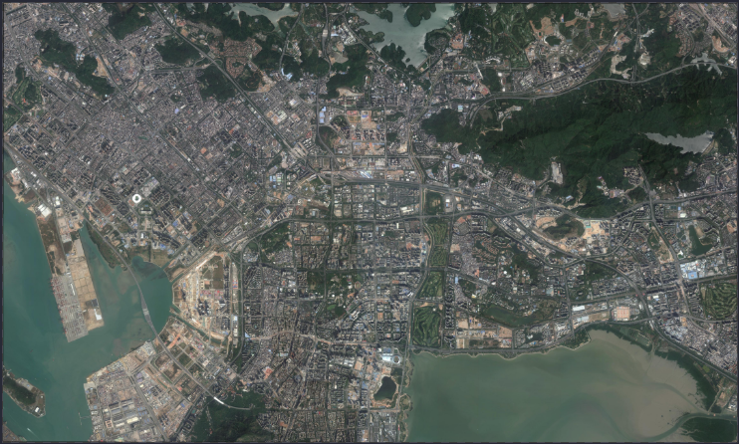
\includegraphics[scale=0.7]{figure/F5}
%  \caption{大GSD遥感图像}\label{F5}
%\end{figure}
%
%\begin{figure}
%  \centering
%  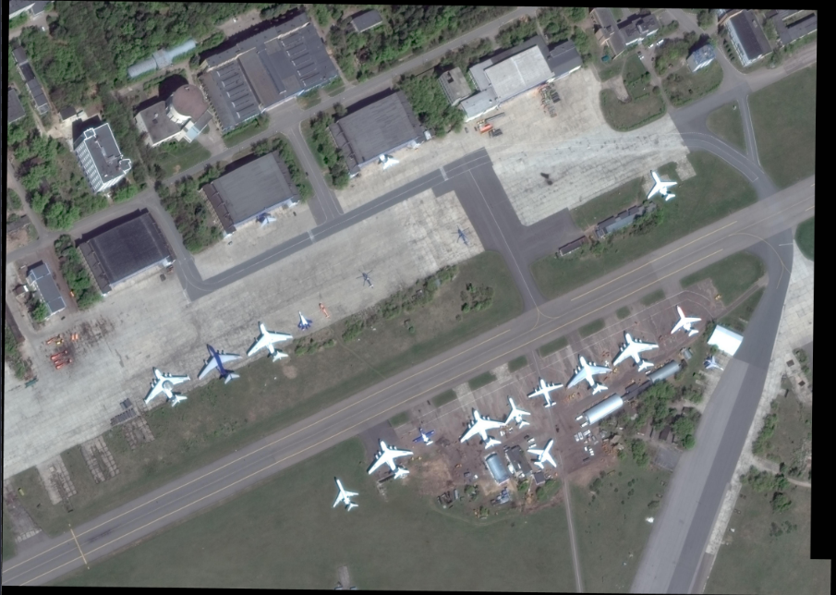
\includegraphics[scale=0.7]{figure/F6}
%  \caption{小GSD遥感图像}\label{F6}
%\end{figure}
%
%\section{算法设计}
%
%网络整体结构如图\ref{F29}所示,网络主要由三个子模块网络构成,分别是GSD预测网络、超分辨网络及目标检测网络。GSD预测网络可以接收完整的待检测遥感图像,通过对图像纹理复杂度的分析,输出对图像GSD大小的判断结果;而超分辨网络则接收来自GSD预测网络的输出与输入的遥感图像,按照预测结果对图像进行分割和选择性的超分辨,得到若干图像序列;最后,目标检测网络接收前端网络标准化之后的输出作为输入,基于两步法思想执行目标的定位与检测任务,它的输出即为网络的最终输出检测结果。
%
%\begin{figure}
%  \centering
%  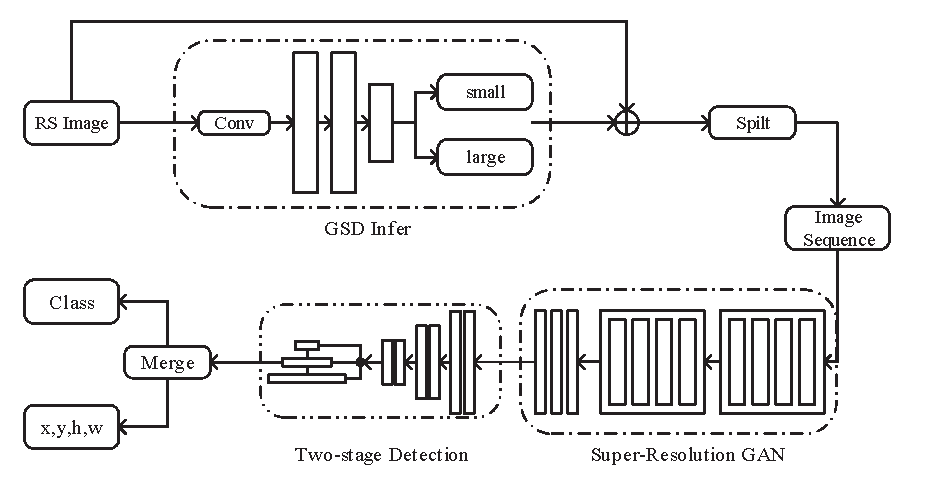
\includegraphics[scale=1]{figure/F29.eps}
%  \caption{网络整体结构}\label{F29}
%\end{figure}

%\subsection{GSD预测网络}
%
%在计算机视觉领域,图像复杂度(Image Complexity)可以从多个维度进行评估,如色彩复杂度(Color Complexity)、纹理复杂度(Texture Complexity)与形状复杂度(Shape Complexity)\cite{31周兵2018图像复杂度研究综述}。在遥感图像中,GSD的大小决定了像素所代表实际地面距离,可以推断出,GSD间接地决定了在遥感图像中一个单位像素块所包含的实际区域大小,显然地,GSD越大,对于同样的地理区域而言,图像所涵盖的区域内建筑、目标、背景环境就越复杂,而这一复杂性可以通过图像的纹理复杂度得以体现,因此一种基于遥感图像纹理复杂度的GSD预测网络应运而生,其整体算法流程如图\ref{F17}所示,主要由预处理、纹理提取和距离估计三部分构成。
%
%\begin{figure}
%  \centering
%  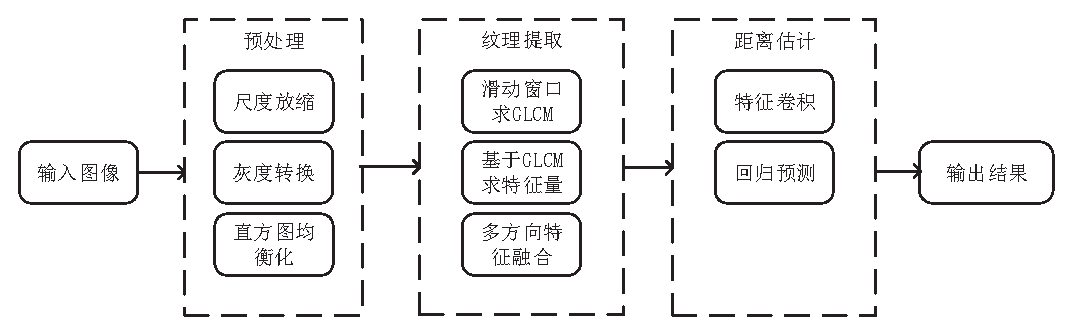
\includegraphics[scale=0.8]{figure/F17.eps}
%  \caption{GSD预测网络}\label{F17}
%\end{figure}
%
%\subsubsection{预处理}
%
%预处理环节在提取遥感图像纹理特征之前先对输入图像进行一定的处理,使其能够符合后续处理的尺度、色彩要求,避免结构性误差的引入。一般地,基于输入图像特性,从以下几个方向进行预处理:
%
%1.尺度放缩。遥感图像往往具有常规意义上的过大分辨率,而在进行图像的纹理特征提取与GSD预测时,需要确保输入的完整性,防止因局部平滑导致的误判和错漏。因此对图像的尺度进行放缩是很有必要的,这样就能利用图像的尺度不变性特征,在计算量较小的情况下进行纹理提取工作,降低了不必要的资源消耗,提升了网络整体运算效率;
%
%2.灰度转换。多通道图像会使得图像的纹理提取工作更为复杂,但与此同时却不能显著增强提取出的纹理特性,因此基于优化网络结构、提升网络计算效率的目标,可以将输入的彩色图像以一定方式转化为灰度图像,具体计算方式如式\ref{equ6}所示,其中R、G、B分别代表图像RGB通道对应像素值,该转换方式是由计算机图像处理及人眼视觉感知的通用准则规定而成,以认知心理学对于RGB图像色彩的研究为基础,可以最大程度的确保灰度图像与原图像在视觉感知、图像处理中的一致性。
%\begin{equation}\label{equ6}
%  Y=0.299R+0.587G+0.114B
%\end{equation}
%
%3.灰度直方图均衡化。这是一种传统的灰度图像处理方法,其目标是使得图像灰度分布更为均衡地分布在整个灰度域之上,使图像的亮暗都更加明显,增强了对比度。在图\ref{F18}中,图(a)为原灰度图像,图(b)为经过直方图均衡化之后的灰度图像,相比于原图,均衡化使得图像中明度对比度得到增强,图像细节进一步凸显,纹理更加清晰,便于后续处理。
%
%\begin{figure}
%  \centering
%  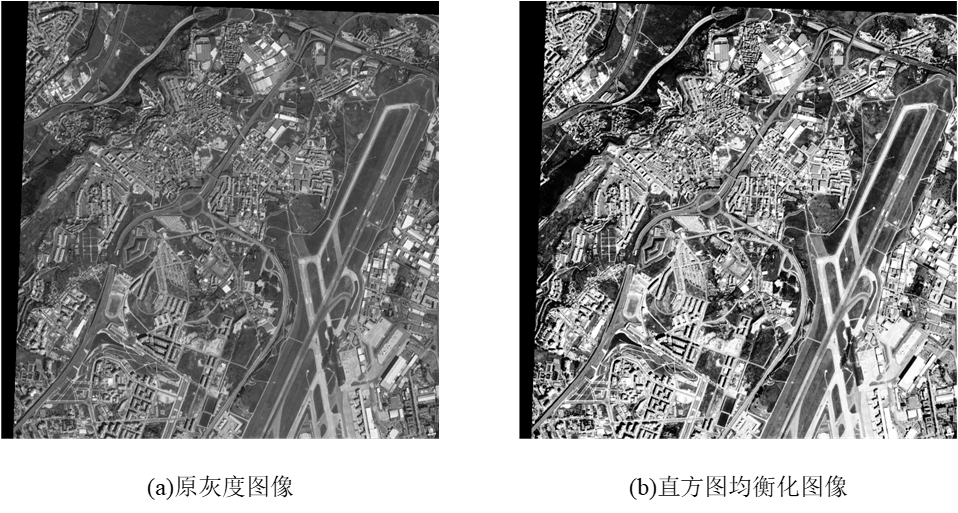
\includegraphics[scale=0.5]{figure/F18}
%  \caption{直方图均衡化}\label{F18}
%\end{figure}
%
%\subsubsection{纹理提取}
%
%在图像分析领域,常常通过计算灰度共生矩阵及其特征值(Gray-Level Co-occurrence Matrix, GLCM)\cite{34haralick1973textural}来对图像的纹理复杂度进行评估。在文章中,灰度共生矩阵被定义如下:设一灰度图像具有\emph{N}个灰度值,那么计算得到的灰度共生矩阵的大小就为\emph{N×N}阶,规定一个像素对偏移量为δ,它意味着计算时需要不断地在图像中按角度θ去遍历距离为δ的像素对\emph{a}、\emph{b},可以得到其灰度值对(\emph{a$_{k}, b_{k}$}),随后将具有相同灰度值对的像素对数量累加,对应着灰度共生矩阵中(\emph{a$_{k}, b_{k}$})的元素\emph{G}(\emph{a$_{k}, b_{k}$})的值。当遍历完整个图像之后,就得到了该图像对应的灰度共生矩阵G。
%
%\begin{figure}
%  \centering
%  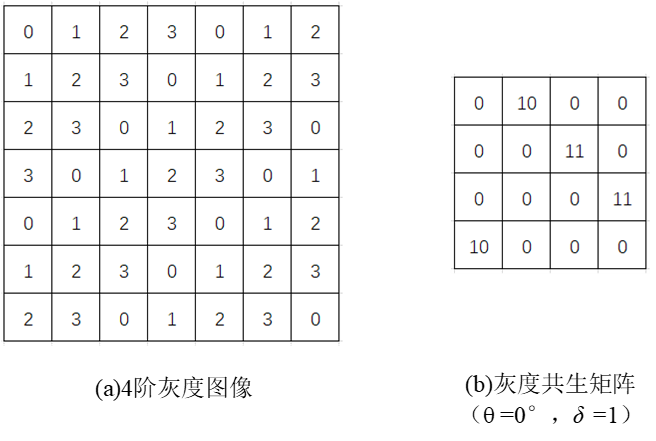
\includegraphics[scale=0.6]{figure/F19}
%  \caption{灰度图与灰度共生矩阵}\label{F19}
%\end{figure}
%
%如图\ref{F19}所示为一幅具有4阶灰度级的灰度图像及以水平方向进行遍历得到的灰度共生矩阵,显然地,灰度共生矩阵是基于像素对灰度值的统计量,它记录了在图像当中不同灰度匹配模式的出现次数,而δ则代表了该灰度共生矩阵对于灰度纹理精细级别的敏感度,当δ越小时,像素对间距较小,则检测的纹理较细致,反之则纹理越粗糙。
%
%进一步的,当使用不同的距离δ与遍历角度θ时,可以得到设置不同方向与不同距离时的灰度共生矩阵如图\ref{F20}所示。这体现了灰度共生矩阵对于纹理方向的敏感性。一般地,为使提取到的纹理特征具有一定的旋转不变性,会特别地使用0°、45°、90°、135°这四个角度进行计算,距离则由图像中主要纹理的粗糙程度来定义。
%\begin{figure}
%  \centering
%  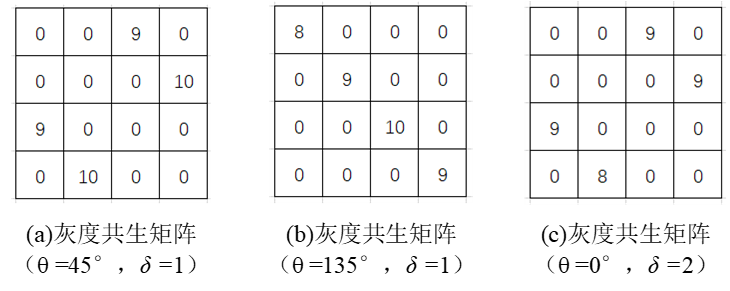
\includegraphics[scale=0.5]{figure/F20}
%  \caption{不同条件下的灰度共生矩阵}\label{F20}
%\end{figure}
%
%灰度共生矩阵具有着图像的纹理统计信息,但就作为图像纹理特征而言,其鲁棒性尚不能满足要求,不够直观也是一个巨大的不足,研究者们难以直接利用灰度共生矩阵进行比较和分析。因此,在提出灰度共生矩阵的同时,Haralick团队也给定了14个用于纹理分析的计算统计量,也即纹理描述子,分别为:二阶矩、熵、对比度、均匀性、相关性、方差、和平均、和方差、和熵、差方差、差平均、差熵,同质性及最大相关系数,但彼时他并未给出这些统计量的有效性与相关性结论。随后,Barald\cite{39baraldi1995investigation}等人经由研究计算论证,说明在Haralick给出的14个统计量中,其中4个统计量之间不相关性最强,对于遥感图像具有较好的特征表现能力。分别是:
%
%1.	二阶矩(Angular Second Monment, ASM),也被称作能量,其计算方法由式\ref{equ8}给出,其中\emph{P}(\emph{i, j})为灰度共生矩阵中位于(\emph{i, j})处的元素归一化概率。ASM对灰度共生矩阵内值的和大小敏感,当图像纹理分布均匀、纹理粗细程度接近时,ASM可以获得较大值;
%\begin{equation}\label{equ8}
%  Asm=\sum_{i}^{}\sum_{j}^{}P(i,j)^{2}
%\end{equation}
%
%2.	熵(Entropy, ENT),在物理学领域中,熵被用来描述一个系统的混乱程度。在此处,其计算方法由式\ref{equ9}给出,它具有类似的描述功能,可以用于表现图像中纹理的复杂程度或分布的非均匀程度,当熵值越大时,意味着图像中纹理随机性较强、分布较为复杂,显然地,对于一张纯色图像,其熵值为0;
%\begin{equation}\label{equ9}
%  Ent=\sum_{i}^{}\sum_{j}^{}P(i,j)logP(i,j)
%\end{equation}
%
%3.	同质性(Homogeneity, HOM),也被称为逆方差。其计算方法由式\ref{equ10}给出,正如其名,同质性关注的是图像中局部区域的纹理变化情况,当不同区域间的图像纹理变化较为缓慢平滑时,其值较大,反之较小的同质性意味着不同区域间纹理变化剧烈;
%\begin{equation}\label{equ10}
%  Hom=\sum_{i}^{}\sum_{j}^{}P(i,j)^{2}/[1+(i-j)^{2}]
%\end{equation}
%
%4.	非相似性(Dissimilarity, DIS),这是一类用于度量图像局部或整体区域内灰度差异区分度的统计量,其计算方法由式\ref{equ11}给出,通过公式可以发现,DIS与灰度间的度量具有线性关系。
%\begin{equation}\label{equ11}
%  Dis=\sum_{i}^{}\sum_{j}^{}P(i,j)|i-j|
%\end{equation}
%
%除此之处,基于对图像信息的提取需求,还有另外几类较为直观的统计量也常常被用于计算之中,如均值、对比度及相关性等,其中均值表征了图像中灰度的整体或局部明暗度,当图像中出现规则、易于描述的纹理时,均值将具有较大值;对比度是对图像中局部像素与其周围像素的灰度差距的度量,灰度共生矩阵对比度与图像对比度表征类似,越大对比度的图像说明在图像中纹理越清晰,边界较明显\cite{40高程程2010基于灰度共生矩阵的纹理特征提取};相关性则具有方向敏感性,其与计算时遍历图像的方向有关,它揭示了在图像中沿着某一特定方向上灰度纹理的延伸长度,与非相似性DIS类似,它也是一个灰度关系的线性度量统计量。
%
%需要更进一步指出的是,上述的所有统计量都是标量形式,在一些简易灰度图像处理方法中,往往将这类统计量进行联合,构建一个多维矢量对图像进行纹理的表征,称之为特征矢量,然后利用特征矢量代入计算之中执行相似性对比、分类等任务。但在遥感图像中,这一方法存在若干不足之处,其一是遥感影像更为复杂,由于其覆盖广阔,影像中会存在多种地块与丰富的目标,单一统计量在复杂图像中显得较为乏力,区分维度不够,无法表征出图像局部纹理特征,如水域与城市共存时,即无法体现出水域的统计特性,也难以表征城市建筑的纹理特征,使得不同地域、不同纹理下的遥感图像在特征矢量中差异性较小、边界不易区分,严重降低了遥感图像纹理特征的表征能力与可识别性。因此,借由卷积神经网络的启发,在本设计中,将滑动窗口思想应用于灰度共生矩阵的计算当中,使用了基于局部灰度共生矩阵的特征图表征方法,该算法主要有以下步骤构成:
%
%1.	设置一个7×7的滑动窗口,padding为3,步长为1,窗口起始位于图像左上角;
%
%2.	针对滑动窗口中的7×7图像区域以前述定义的计算方法进行统计,得到对应的局部图像灰度共生矩阵;
%
%3.	计算得到的局部灰度共生矩阵中均值、方差、同质性、对比度、非相似性、熵、能量、相关性和自相关等一系列统计量,分别输出作为该滑动窗口的输出,其输出形式为多维度矢量;
%
%4.	将滑动窗口按照既定的步长,以从左至右,自上而下的轨迹对遥感图像进行遍历,每次移动后重复第2、3步骤得到输出;
%
%5.	待滑动窗口遍历结束,将期间的所有输出按统计量类别组合,可以得到多幅特征图像,图像与原输入图像具有相同的分辨率,但仅仅表征了图像的灰度共生矩阵在某一特定统计量下的表现;
%
%6.	重复1至5的步骤,但在计算灰度共生矩阵时,分别使用0°、45°、90°、135°对纹理进行统计;
%
%7.	将同一图像中同一纹理统计量在不同计算角度下的特征图以平均加权的方式进行加和,得到最后的特征图像,由于本网络中设计了9类统计量表征纹理特性,因此得到H×W×9维度的纹理特征图像,其中H、W为输入图像的高与宽。
%\begin{figure}
%  \centering
%  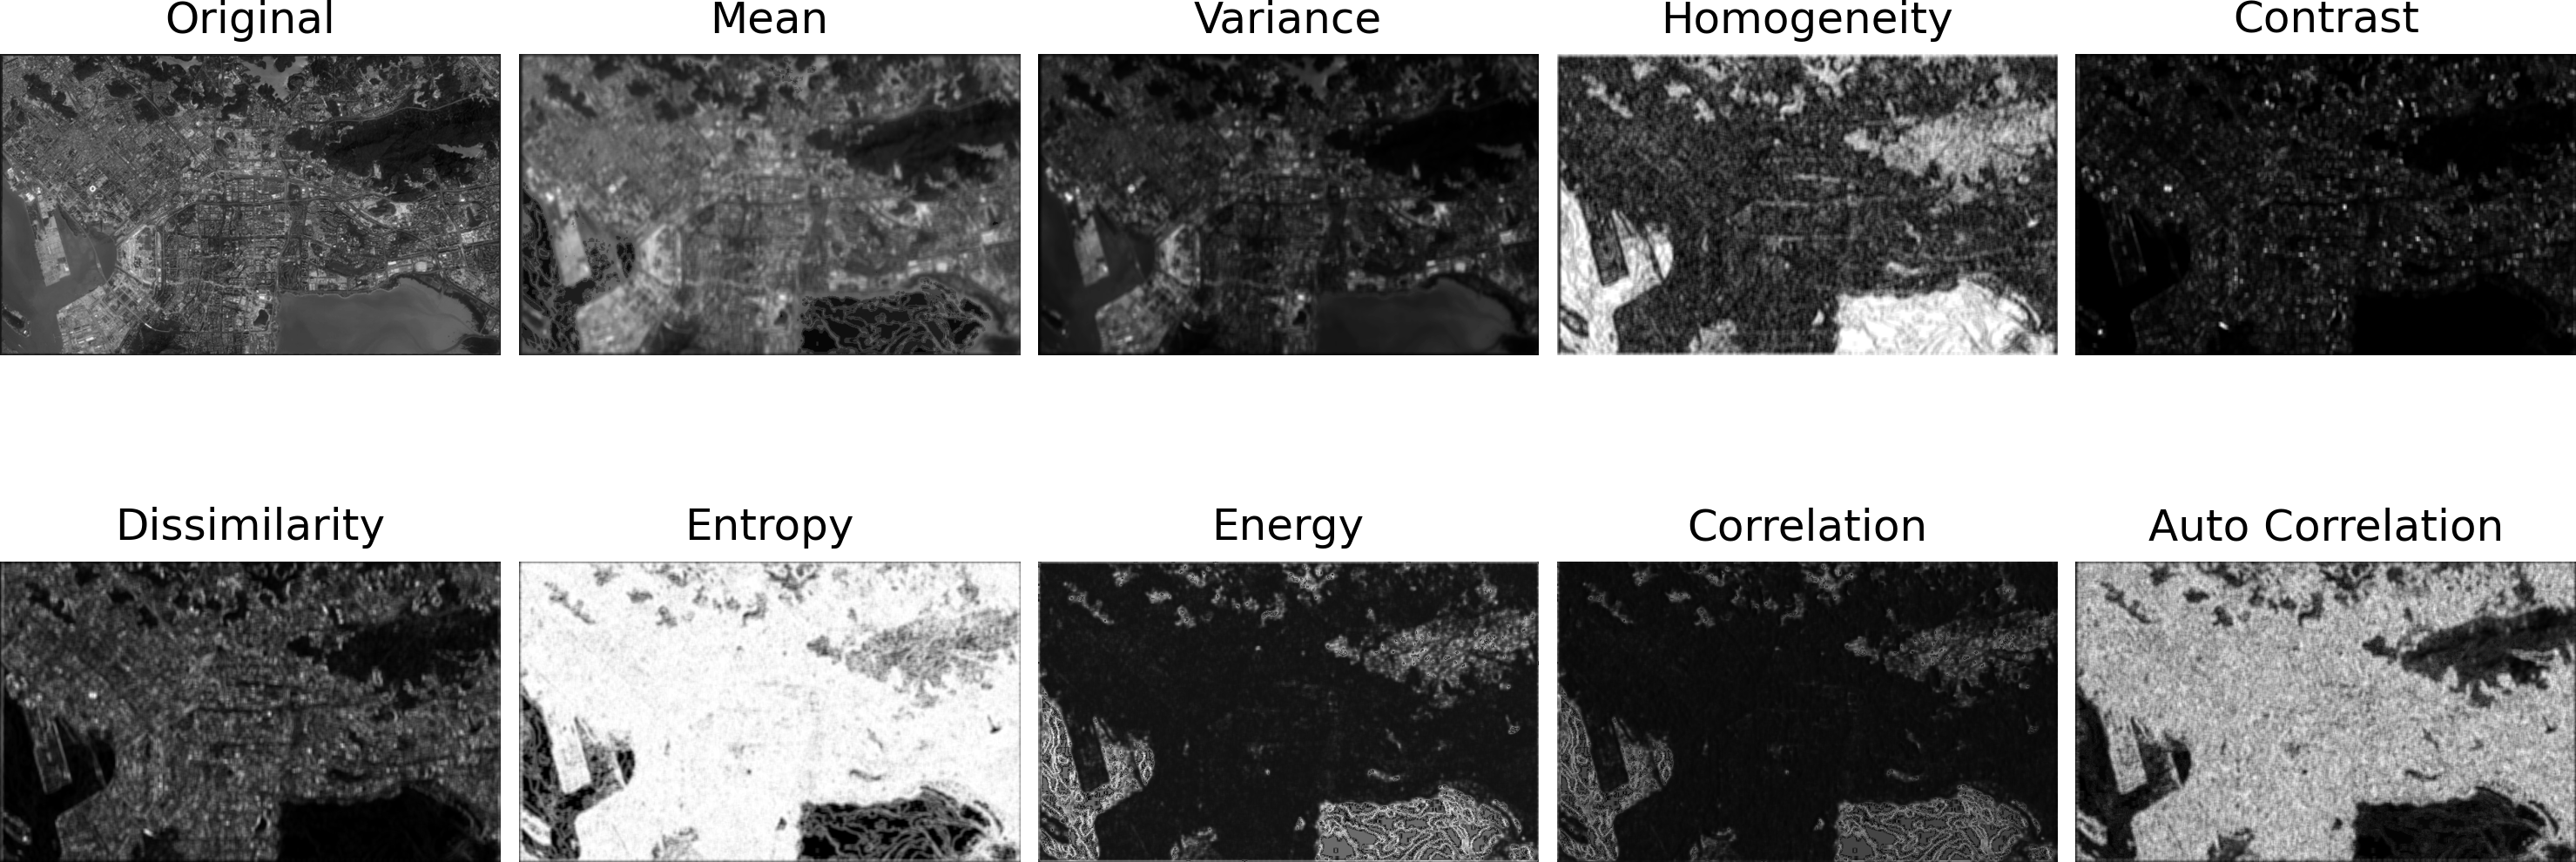
\includegraphics[scale=0.5]{figure/F21}
%  \caption{大GSD图像GLCM}\label{F21}
%\end{figure}
%
%\begin{figure}
%  \centering
%  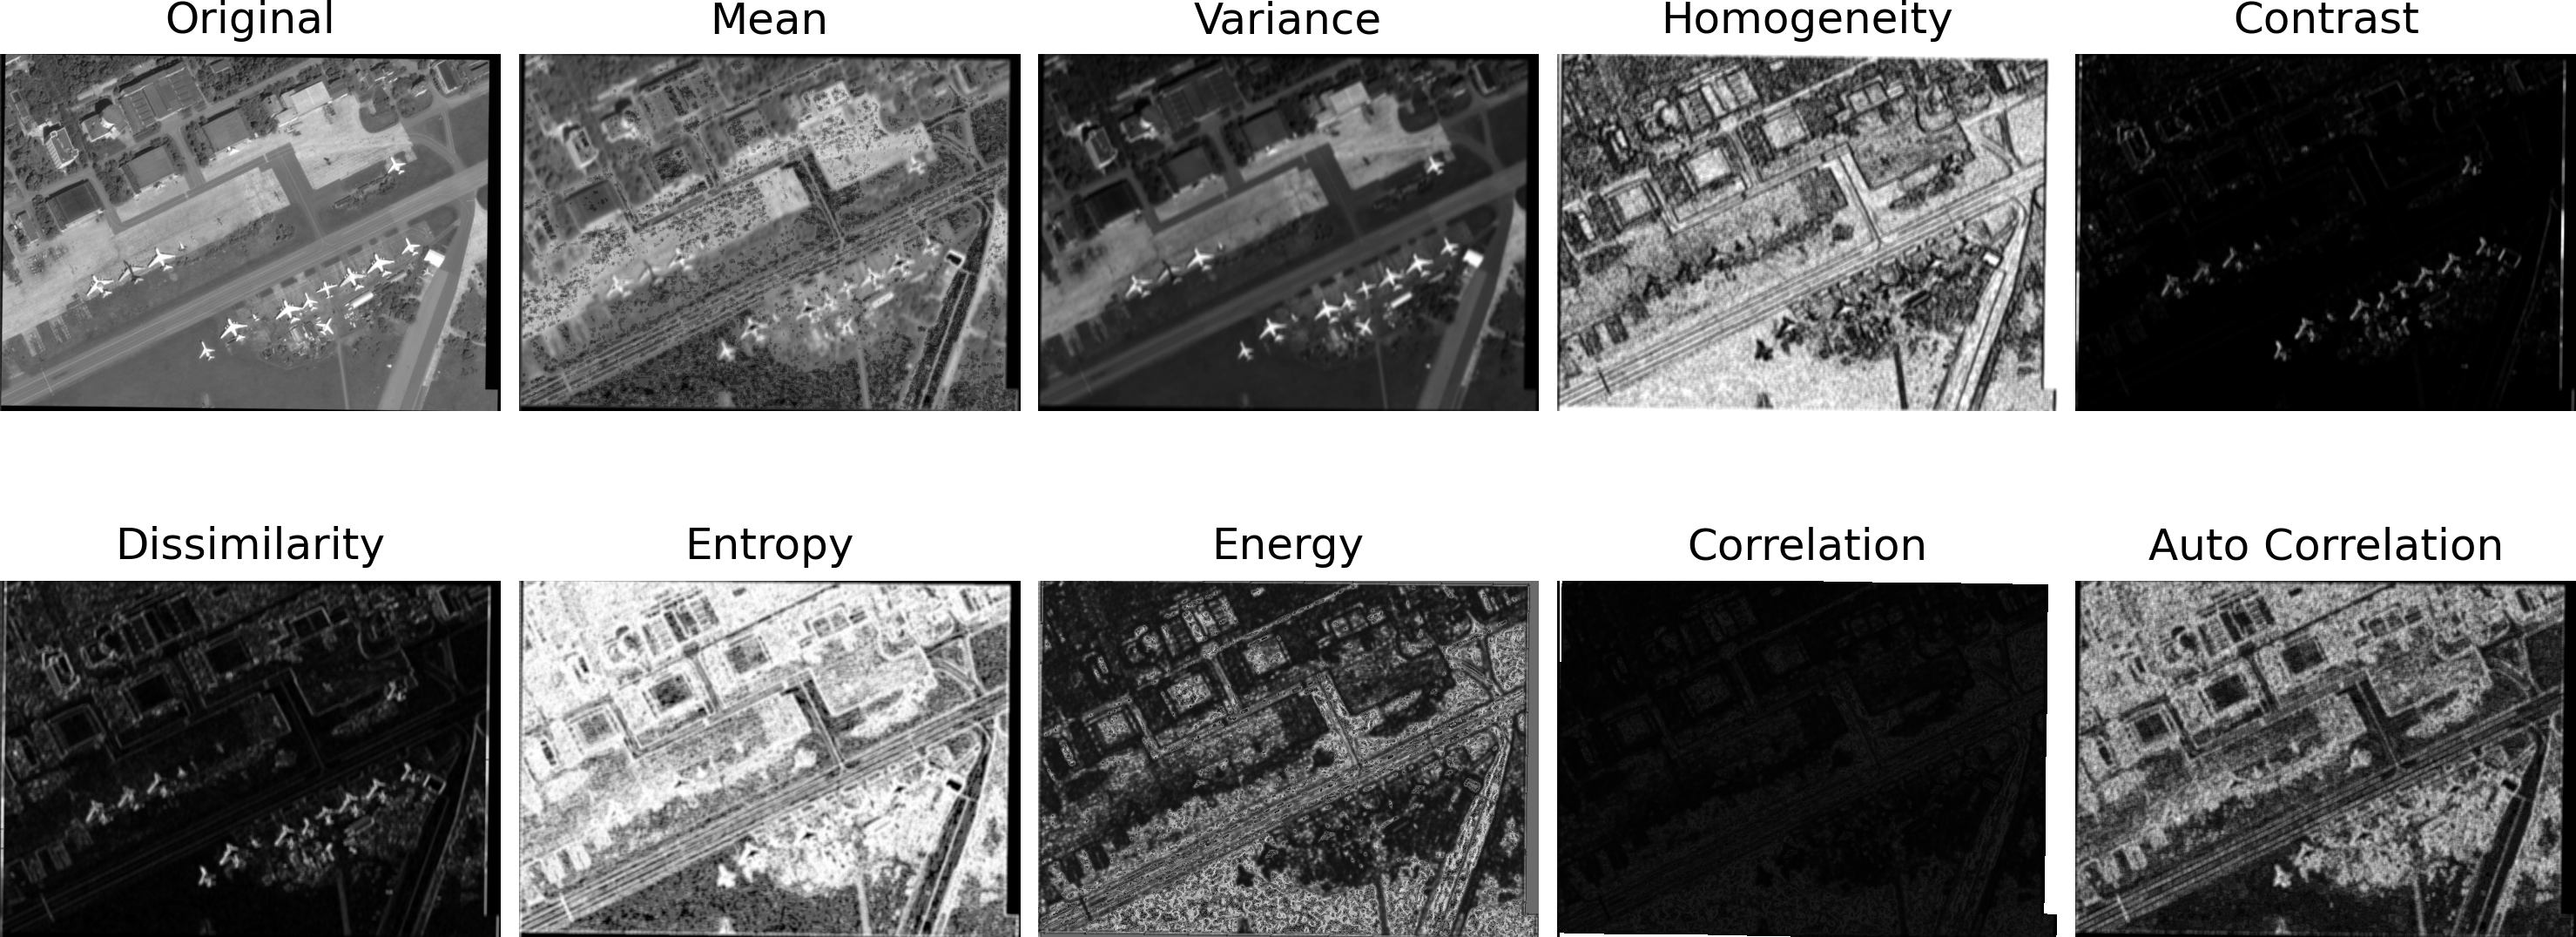
\includegraphics[scale=0.5]{figure/F22}
%  \caption{小GSD图像GLCM}\label{F22}
%\end{figure}
%至此,获得了一幅输入遥感图像的纹理特征图,它同时具有着局部特征与整体特征的信息,且在多个方向上都具有一定的纹理敏感性,最大程度地提取了图像中由不同地块、不同目标和不同区域所产生的纹理特征,为评估图像复杂度提供了坚实依据,为后续GSD预测提供了可靠鲁棒的输入。图像\ref{F21}和图\ref{F22}给出了对图像\ref{F5}和图\ref{F6}的纹理特征提取图结果。
%
%
%
%\subsubsection{距离估计}
%
%距离估计网络的设计目标是通过学习图像的复杂度,尤其是纹理复杂度的信息,合理推测出图像拍摄时的GSD参数状态。各领域研究者也曾提出过相应的方法来利用灰度共生矩阵信息,如Wed等人便利用GLCM与K-means聚类算法相结合,试图以无监督的方式对医学影像中的病症点进行分析\cite{41oleiwi2018alzheimer};还有Naveena等人则将GLCM与SVM分类器相结合,在树叶分类问题中取得了显著表现\cite{42vidyashanakara2018leaf}。然而,在遥感图像领域,这类方法效果却并不尽如人意,这是因为遥感图像具有较大分辨率与较为丰富的图像内容,在简单线性分类方法中会带来过高维的复杂度,占用过多计算资源。
%\begin{figure}
%  \centering
%  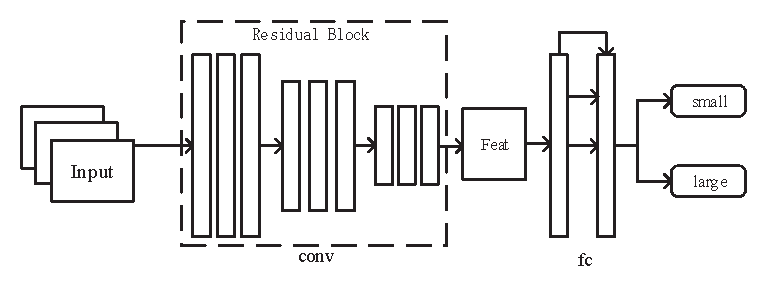
\includegraphics[scale=1.2]{figure/F23.eps}
%  \caption{预测网络结构}\label{F23}
%\end{figure}
%
%因此,基于对输入图像内容的复杂性进行估计的需求出发,本章节中提出了一种使用深度卷积网络提取特征并回归分类预测遥感图像GSD的方法。网络结构以ResNet-50为基础进行修改,因为其深度能够满足特征提取与学习的需求。具体结构如图\ref{F23}所示,输入图像为前述计算所得到的纹理特征图像块,在输入网络前,为满足网络卷积输入条件,需要先将其尺度调整为224×224,随后设计了多个残差卷积块,每个残差块由1×1和3×3的多个卷积核叠加而成,最终展平后得到1×1×4096维的特征图像,在池化层利用平均池化方式进行降维后,直接与全连接层FC1相连,FC1具有2048个神经元,它的输出经由密集全连接输入全连接层FC2的512个神经元,最终汇集为两类输出,完成回归分类并输出标签。基于本次使用数据集DOTA中的图像GSD实验特性,当GSD较小时,检测网络对目标仍能具有较好的适应性,而当GSD过大时,网络无法识别出其中的极小目标,因此在GSD预测输出中将图像分类为正常GSD尺度与过大GSD尺度两类。网络使用Adam优化器进行反向梯度传播,损失函数为交叉熵损失,如式\ref{equ12}所示,在本网络设计中\emph{N}为2,\emph{L$_{i}$}为单一类别的交叉熵损失 。
%
%\begin{equation}\label{equ12}
%  L=\frac{1}{N}\sum_{i}^{}L_{i}=\frac{1}{N}\sum_{i}^{}-\sum_{c=1}^{M}y_{ic}log(p_{ic})
%\end{equation}
%
%在进行网络设计时,曾经存在着另一方案的设计,即将GSD准确值或近似值作为回归的预测目标。但经过实验证明,这一方案存在两个不足之处:其一是GSD与图像复杂度特征间为非线性关系且不具有强烈相关性,对于遥感图像这类具有较高复杂度的图像而言,要将其与单一精确数值进行关联是非常困难的;其二是由于后续需要使用超分辨等图像尺度变换操作,为确保其输出效果准确,对于图像输入尺度与放缩比例具有严格要求,无法直接利用预测出的精确值进行操作,防止在超分辨过程中引入不必要噪声干扰检测结果。因此,综上两点所述,使用分类预测方案,对遥感图像的GSD值进行预测是一个能在检测效率、识别准确率及资源利用率上达到平衡的方法,具备一定的优势。
%
%
%\subsection{图像超分辨}
%
%前述对图像的分析与预测工作,其最终目的都在于提取遥感图像的GSD信息,并将其引入网络之中。在本节中,正是出于对GSD信息的利用方法进行思考,设计了一个遥感图像超分辨网络,其逻辑意义在于:基于图像\ref{F5}和\ref{F6}的分析可以发现,当在不同GSD图像中取同样大小像素块时,对于图像中的同类目标,其体现在像素尺度之上的差距正是两图像GSD的比值,此外,研究者们的一致认知是,对于现有的遥感目标检测网络而言,由于其训练时大部分目标都分布于正常GSD尺度之下,网络学习到了这一尺度敏感性,所以难点之一便是在大GSD图像中出现的极小目标,其尺度比正常尺度下的同类目标缩小了数倍,故难以被网络检出。因此,一个利用GSD信息的方法便自然地产生,即将大GSD图像通过某种方式进行放大,人为地调整图像GSD的大小,使之接近正常GSD图像,从而增大对大GSD图像中极小目标的检测能力。
%
%传统的图像放大方法主要有插值类方法,其主要原理是参考原低分辨率图像中的相邻像素值,对得到的高分辨率图像中空白像素进行填充,根据插值内核处理方法不同可以分为线性插值方法如最邻近插值、双线性插值和三线性插值等方法,和非线性插值方法如基于边缘信息的插值方法、基于小波系数的插值方法等\cite{43钟宝江2016图像插值技术综述};而超分辨网络方法则是基于神经网络学习的方法,其所利用来超分辨的信息并不局限于单一输入图像,而是基于多幅图像的学习结果来估计目标高分辨图像的像素值,超分辨网络得到的图像像素与原低分辨图像间并不存在严格的位置映射关系,严格来说,新图像中每一个像素都是重新计算得到,不会保留原有图像中像素的所有信息。传统方法较为简单,运算速度快,且能适应更为灵活的图像放大倍率,但它只能基于输入图像中所具有的像素信息进行放大,对于大型图像或较为复杂的图像,其输出图像在视觉效果及噪声检测指标上都存在不足;而超分辨类方法则能适应复杂图像的放大任务,但需要使用大量已知标定数据进行预先训练,且计算时间相对较长,由于网络结构的限制,对放大倍数和输入尺度存在限制,只有在预设倍数和尺度下工作时才能发挥网络的最佳性能。综合这两类方法的优劣,在本网络中,针对遥感图像显然使用超分辨网络更为合适,而在之后的实验中也证明了这一点。
%
%\begin{figure}
%  \centering
%  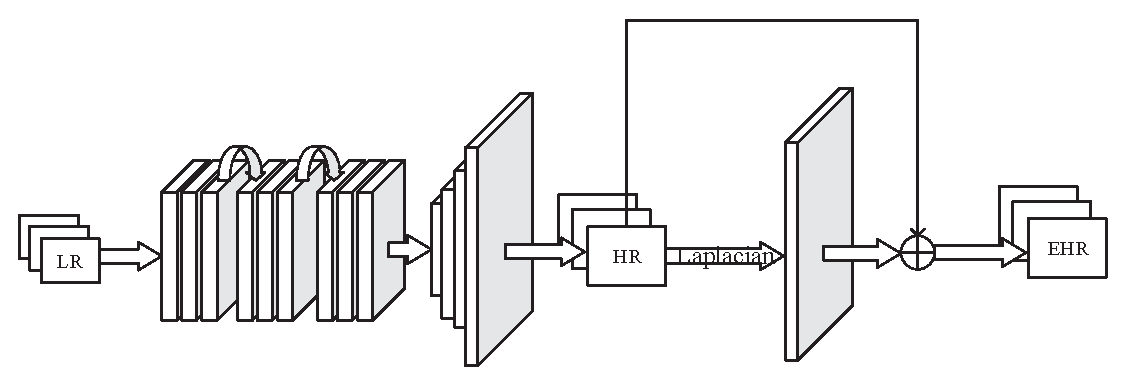
\includegraphics[scale=0.6]{figure/F24.eps}
%  \caption{超分辨网络结构}\label{F24}
%\end{figure}
%本章所使用网络结构为对抗生成网络(Generative Adversarial Network, GAN),最初的GAN结构是由Goodfellow\cite{44goodfellow2014generative}提出,GAN网络正如其名,具有“生成器”与“判别器”之间的对抗过程,生成器以某一规则不断生成与真实样本相似的样本或分布,如音频样本、图像样本和文本样本等,而判别器则被设计成为具有类似特征提取与识别功能的网络,它需要将生成样本与真实样本进行区分,这两部分互相拮抗,通过构建相关联的损失函数进行相互优化。而在超分辨任务中,生成器的任务便是基于原始低分辨率图像(Low Resolution, LR)生成高分辨率图像(High Resolution, HR),经由判别器与原高分辨率图像对比得到误差,不断优化生成图像质量,从而实现图像超分辨。如图\ref{F24}所示即为本网络中使用的超分辨网络的示意结构,首先以超分辨网络SRGAN\cite{45ledig2017photo}的生成器结构为基础,考虑到遥感图像的特殊性,泛用的超分辨方法很容易导致输出的图像中出现地面细节部分的模糊,严重影响到遥感目标的检测与定位,因此在后端加入一个边缘提取网络对得到的高分辨率图像进一步增强,并把增强后具有边缘信息的边缘增强高分辨图像作为网络的最终输出,其具体的操作步骤如下所述:
%
%1.	首先将需要超分辨遥感图像进行尺度裁剪至预定大小的多张图像,获得尺度一致的输入低分辨率图像LR;
%
%2.	利用多个残差块构建生成器网络,每个残差块结构如图\ref{F25}所示,包含有两个3×3×64的卷积层,其步长为1,在卷积层之后加入批归一化处理(Batch Normalization, BN)与PReLU(Parametric Rectified Linear Unit)作为激活函数;由多个残差块进行连接,在此过程中特征特图块的通道数逐渐增长,从广义上看便是逐渐学习到了高分辨图像所缺失的内容,最后连接3×3×256卷积层并进行维度变换,得到3通道放大尺度图像,达到了对图像进行上采样的目的,并输出高分辨率图像HR;
%\begin{figure}
%  \centering
%  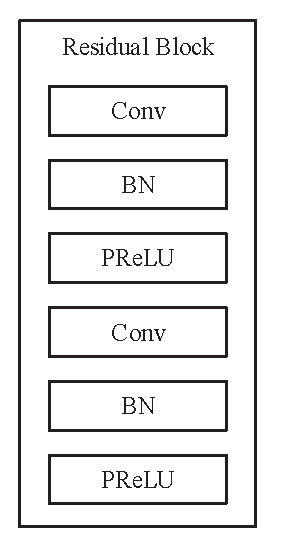
\includegraphics[scale=0.8]{figure/F25.eps}
%  \caption{残差块}\label{F25}
%\end{figure}
%
%3.	将高分辨率图像HR再次作为输入,首先进行灰度转换得到灰度图像,随后使用一个低通滤波器对图像进行滤波,消除原本存在的部分高频噪声;最后再使用拉普拉斯算子提取高频边缘信息,得到边缘图像;
%
%4.	最后将边缘图像与生成的高分辨率图像HR融合,融合方法为将HR图像的三通道图像分别与得到的边缘图像进行加权求和后归一化,获得具有强边缘效果的高分辨率图像EHR,其尺度与最初生成的高分辨率图像一致,并具有更清晰的边缘信息,虽然无法完全恢复原图像中的边缘信息,但后续实验证明,其输出EHR在检测效果上已优于HR。
%
%
%\subsection{目标检测网络}
%
%目标检测网络采用了上一章节中所构建的基于Faster-RCNN加入可形变卷积与级联结构的两步式遥感目标检测网络,其在实验中取得了最佳表现,非常适合作为后端的目标检测网络,其具体结构原理与检测能力已经在上一章节中进行了详细说明,此处不再赘述。
%
%\section{本章小结}
%
%在本章中,提出了一种能够利用遥感图像GSD信息进行超分辨的目标检测网络,经由实验证明,GSD可以作为遥感图像的特殊信息引入检测网络之中,通过计算遥感图像复杂度特征图与之建立关联,并依据数据集分布将这一信息转化为图像放大倍数的依据,再利用超分辨网络进行图像尺度上的放大。在实验中,这一方法取得了对于大GSD图像中小目标检测准确率的提升,同时了降低了目标遗漏与目标检测框定位过大问题的出现概率,检测指标与检测结果可视化的展示皆证实了这一方法的有效性、合理性与必要性,为进一步提升遥感图像中小目标检测能力提供了新的见解。


\chapter{遥感目标分割问题研究}
\section{图像分割主流算法}

目前图像分割领域主要研究方向分为两个方面:传统分割方法和深度学习方法。

\subsection{传统分割方法}

1.基于阈值的分割方法
根据我们获得的遥感图像,取一个合适的灰度阈值,将分类好的像素点归为同一类。通常遥感图像中有多个目标需要检测,因此也需要提供多个阈值将目标分割开来。优点在于算法简单且运算速度快,但无法判断噪点和真实图像的差异,对遥感图像的数据纯净度要求较高,鲁棒性较差。

2.区域生长以及区域分裂合并
区域生长是让一系列处于不同类别区域的像素种子生长,种子逐渐将近邻且符合相似条件的像素点合并,最终形成一个完整的区域。区域分裂合并是让一个完整的图像逐渐分割,直到任何一个子区域中没有其他类别的目标元素组成,再将具有相同类别特征的子区域合并,从而分割出遥感图像中不同类别的目标。难点在于如何指定合适的判决准则来精确分割目标的边界。

3.边缘检测算法
边缘检测算法也是图像处理中最为常见的算法之一。我们可以将遥感图像通过傅里叶变换到频率域,高频就代表着该图像的边缘部分。通常使用一阶或者二阶导数来探索图像的不连续性,从而对遥感图像进行精确的分割。该领域的相关算法精确度较高,但同时也对图像有着严格的要求。如果不能保证边缘的连续性和封闭性,不能准确分辨出重要边缘和假边缘,该算法的效果将大打折扣。

\subsection{深度学习方法}

1.基于区域选择
在RCNN的基础之上,人们提出了Mask-RCNN以及Mask Scoring RCNN来完成像素级别的图像分割。它分为两个阶段,第一个为RPN(区域提议网络)阶段,提出候选目标边界框。第二个阶段就是它的前身Fast R-CNN,使用RoIPool从每个候选框之中提取特征,并为每一个ROI输出二进制掩码,从而对遥感图像进行分类和回归。这两个阶段部分参数特征都是共享的,这样也保证了运行的速度快。

2.基于RNN的图像分割
RNN是由Long-Short-Term Memory组成的网络,在图像分割方面比较经典的模型有ReSeg模型和MDRNNs模型。前者用多个RNN组合在一起,同时使用中值的频率来重新进行加权类的预测,从而有效地降低噪声对遥感图像的影响。后者将RNN拓展到了多维度空间领域,将单个递归链接替换为多个递归连接,从而保证在精度损失不大的前提下,大大降低运行的速度,避免了时间随样本数据的增加而指数增长的问题。

3.基于FCN的图像分割
FCN和上述算法不同,它会先上采样扩大像素点,再全卷积与反卷积。全卷积采用了CNN的网络并对最后的全连接层进行了修改,变成了1x1 卷积来提取特征。反卷积是将小尺寸的遥感图像上采样,从而得到原图像的语义分割。

\section{ResUNet-a算法复现}

在这次项目中,我们的侧重点是对检测算法的优化以及实现,同时对ResUNet-a(Resnet与Unet的结合)的图像分割算法进行了复现。现实中的遥感图像通常背景复杂,存在着较多噪点,难以正确分辨出物体边界信息,因此传统的图像分割算法准确度较差。Unet是经典的分割模型,采用了编码和解码的结构。先对图像进行多次的卷积,在下采样特征提取之后上采样,将处理前的特征与处理后的相融合,直至输出与输入的尺寸相同。因为整个网络是一个大写的U,所以人们称之为U-net。

\begin{figure}
  \centering
  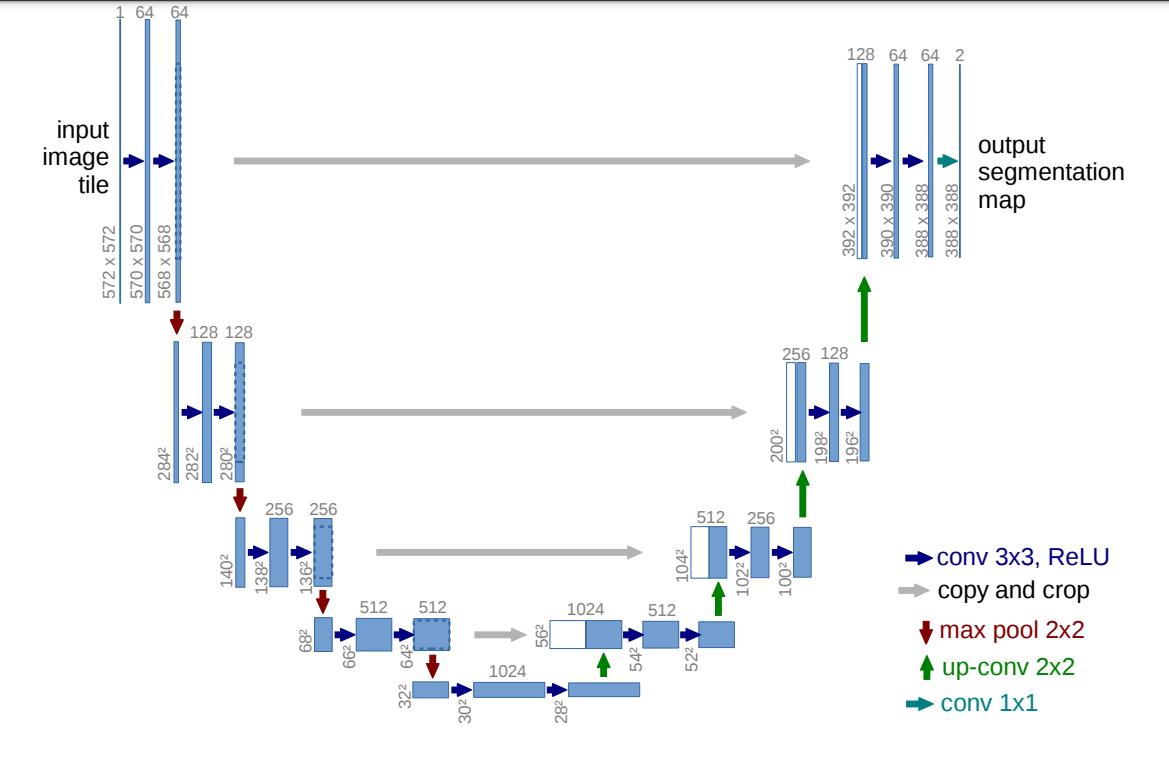
\includegraphics[scale=0.5]{figure/F30}
  \caption{U-net网络结构图}\label{F30}
\end{figure}

相比于上文提到的FCN,它采用的不是特征图的对应像素拼接而是通道数的拼接,从而得到更深的网络层,有着更大的视野域。上下采样的过程中会损失一些权重非常低的特征,而这些特征大部分是遥感原图像存在的噪点。浅层的网络学习纹理特征,深层的网络学习本质特征。在遥感图像中低级特征和高级语义特征同时决定着物体的边界,所以拥有多通道拼接的U-net能有效减少有效信息的缺失。因此Unet在遥感图像上运行速度快,且因为过滤掉较多噪点,准确率也有相应的提升。不过也存在相应的问题,比如多通道导致的数据量大,内存多,容易导致梯度消失和爆炸的问题。

在高分辨率图像中具有尺度变化大,视角特殊等特点。遥感图像从几百米甚至上千米拍摄而来,图像感受野极大,因此会有众多不同类型的目标例如足球场,中型建筑,汽车等。同时由于拍摄遥感图像为高仰空视角,如果不对Unet算法做优化,很难对每种目标都精确分类,甚至产生严重的模型退化效应。模型退化是指:给网络叠加更多的层,性能却有所降低,这是违背我们预期的。越复杂的模型也越难以优化,所以采用Resnet这种残差网络加以改进。如果拟合的函数为F(x),期望的潜在映射为H(x),那么在传统的学习中就是恒等映射。在Resnet残差网络中,我们让它学习残差即H(x)-x,再用F(x)拟合。

\begin{figure}
  \centering
  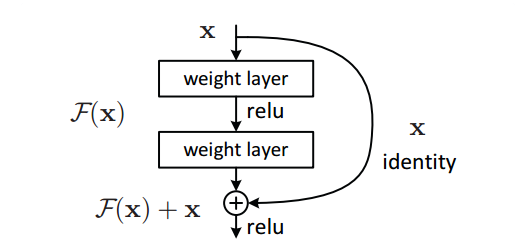
\includegraphics[scale=0.5]{figure/F31}
  \caption{Resnet的框架}\label{F31}
\end{figure}

在此基础上,还可以进一步优化例如添加“bottleneck block”模块,用1x1卷积层先升维再降维,降低计算复杂度,如下图所示。

\begin{figure}
  \centering
  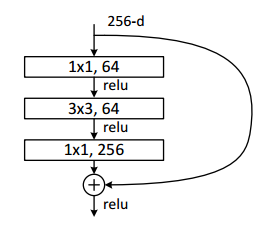
\includegraphics[scale=0.5]{figure/F32}
  \caption{优化后的Resnet}\label{F32}
\end{figure}

同时Resnet为多个Residual Block串联,因此很容易修改数量来得到不同表达能力的网络结构,不用过度担心网络的退化而不敢逐步加深网络的层数。这种方式提取的特征相比于原始特征更容易学习,堆叠层也能在输入特征上学习到新的特征,从而提高模型的精度和稳定性。Resnet和Unet相结合而成的ResUNet-a在遥感图像中有着良好的性能,较好地完成了目标检测与识别后续分割部分的研究。

%\chapter{实验}
%\subsection{实验环境和细节} \label{3.3.2}
%
%本文的所有实验都是在同样的服务器实验环境下进行的,服务器的关键配置信息为:Intel Xeon CPU E5-2697 V3 @2.60Hz 处理器;3块11GB显存的GeForce RTX 2080Ti显卡;Ubuntu 16.04.5 LTS操作系统;CUDA 9.2;采用的深度学习框架为Pytorch 1.15。
%
%在本文实验中根据两个数据集不同的特点在训练和测试阶段对数据进行了不一样的预处理。对于DOTA数据集,由于其中包含的图片分辨率可以达到4000$\times$4000,并且图片中会包含很多小目标类别如SH和SV,直接将图片输入到网络结构中会丢失掉小目标的信息,严重影响检测精度,针对这样的情况,我们在训练和测试的过程中首先对图片进行了切割,对于大分辨率的图片,将其切割成1024$\times$1024大小的子图片块,切割的步长为824,子图片块中不包含任何目标的图片直接删除,对于分辨率不足1024$\times$1024的图片则进行补零操作,经过切割操作之后总的训练图片有6779张。对于HRSC2016数据集,由于不像DOTA数据集一样有大分辨率图片和小目标共同存在的问题,并且HRSC2016数据集中的图片分辨率之间差异不大,所以我们直接在训练中将所有图片固定到同一尺寸大小1000$\times$800。另外为了防止过拟合,在两个数据集的训练实验中都对图片进行了随机翻转。
%
%本文实验的基准网络结构是Faster R-CNN和FPN,在主干网络采用了ResNet-50和ResNet-101进行特征提取,其中在消融实验验证所提出模块的有效性时将ResNet-50作为主干网络,在与一些现有的其他方法进行对比实验时则分别使用了ResNet-50和ResNet-101作为主干网络。在实验设置中,对于FPN输出的每一层特征图(比如P2-P6),不同特征层的候选区域的最初尺寸是其感受野大小的4倍(比如16,32,64,128,256),特征图上的每个特征点位置生成了5个不同长宽比大小(1:1,1:2,2:1,1:3,3:1)的候选区域,在RPN网络输出阶段,保留了2000个得分最高的位置调整之后的候选区域作为感兴趣区域,然后在两级检测网络结构中对感兴趣区域进行正负样本划分时采用了同样的IoU阈值0.5。考虑到数据量大小的不一样,DOTA数据集训练迭代了12步,HRSC2016训练迭代了40步,优化器采用的是带动量的SGD,动量是0.9,权重衰减为0.0001,学习率初始化为0.0025,DOTA数据集训练时在第8步和第11步时分别对学习率进行0.1倍的衰减,HRSC2016数据集训练时在第20步和第30步分别对学习率进行0.1倍的衰减。
%
%\section{改进的多方向级联目标检测方法研究}
%\subsection{消融实验结果分析}
%
%为了验证改进的两级级联结构、多方向RoI对齐模块和方向注意力模块对于本章提出算法检测性能的影响,本小节基于DOTA数据集进行了消融实验分析。如表\ref{tab:3-1}所示,方法1“Baseline”表示的是在原始Faster R-CNN方法的基础上将检测网络中的回归分支输出改为有方向检测框参数,方法2“RoI Align”表示的是引入了两级级联网络结构,并且在第一级检测网络使用传统的RoI对齐进行感兴趣区域特征提取,方法3“M-O RoI Align”表示的是将第一级检测网络中的RoI对齐替换成了本章提出的多方向RoI对齐模块,方法4“M-O RoI Align + OAM”表示的是在多方向RoI对齐的基础上在第一级检测网络回归分支中添加了方向注意力模块,即为本章提出的算法。
%
%\begin{table}
%\caption{\label{tab:3-1}各个改进模块的消融实验结果}
%
%
%\centering{}%
%\resizebox{\textwidth}{!}{
%\begin{tabular}{c|ccccccccccccccc|c}
%  \hline
%  % after \\: \hline or \cline{col1-col2} \cline{col3-col4} ...
%  & PL & BD & BR & GTF & SV & LV & SH & TC & BC & ST & SBF & RA & HA & SP & HC & mAP \\ \hline
%  Baseline & 88.25 & 74.84 & 45.45 & 64.55 & 73.61 & 70.59 & 76.97 & 90.83 & 79.39 & 83.44 & 50.78 & 61.06 & 63.16 & 67.28 & 51.68 & 69.95 \\
%  RoI Align & 88.32 & 76.16 & 50.57 & 69.53 & 73.24 & 72.86 & 85.84 & \textbf{90.88} & 77.68 & 81.86 & 50.44 & \textbf{64.56} & 71.76 & 65.16 & 54.96 & 71.59 \\
%  M-O RoI Align & \textbf{88.81} & \textbf{76.87} & 51.22 & 70.13 & 76.00 & 76.28 & 86.97 & 90.53 & 77.72 & 82.30 & 51.67 & 64.24 & \textbf{74.50} & 68.69 & 55.68 & 72.77  \\
%  M-O RoI Align+OAM & 88.47 & 76.79 & \textbf{53.22} & \textbf{70.47} & \textbf{77.02} & \textbf{77.35} & \textbf{87.03} & 90.83 & \textbf{82.35} & \textbf{82.57} & \textbf{56.19} & 60.39 & 73.88 & \textbf{68.95} & \textbf{55.82} & \textbf{73.22 } \\
%  \hline
%\end{tabular}}
%\end{table}
%
%表\ref{tab:3-1}中展示了各种方法在DOTA数据集上每个类别的检测精度和所有类别的平均检测精度,表中加黑突出显示的是各个类别的最佳检测精度。与方法1“Baseline”相比,方法2“RoI Align”采用了一个额外的检测网络对感兴趣区域进行了转换,mAP总体提升了1.64$\%$,在大部分类别上都有了不小的提升,额外的检测网络转换之后得到的旋转区域对遥感图像中的有方向目标定位更加精确,池化获取的特征更能表示目标,同时旋转区域之间的IoU计算更加苛刻,可以有效排除掉一些可能会出现的假正例检测框,在单一检测目标的精确率和召回率之间做了很好的平衡。
%
%方法3“M-O RoI Align”将前面第一级检测网络中的池化操作RoI对齐替换成了本章提出的多方向RoI对齐模块,从表\ref{tab:3-1}中可以看到,所有类别的mAP提升了有1.18$\%$,尤其是在一些数据集中方向多样的类别如小车(SV)、大车(LV)、码头(HA)和游泳池(SP)有了明显的提升,分别提升了2.76$\%$、3.42$\%$、2.74$\%$和3.53$\%$。多方向RoI对齐模块使用了多个预定义的角度将每个水平感兴趣区域进行旋转,不同角度的旋转区域在池化时对应不同的特征通道集合,最后从每个水平感兴趣区域得到的池化特征对于方向具有一定的鲁棒性,能够有效地缓解不同方向目标带来的特征偏移问题,进一步提升检测精度。但是由于引入了过多不同方向上的特征并且没有对这些特征进行有效选取,在一些方向分布基本水平的目标的检测上表现略微下降。
%
%方法4“M-O RoI Align+ OAM”在方法3第一级检测网络中的回归分支添加了方向注意力模块,实验结果表示所有类别的mAP提升了约0.45$\%$,并且相对于方法3几乎所有类别都有或多或少的提升。方向注意力模块以多方向RoI对齐提取到的多个方向通道集合的特征为基础,在回归分支根据每个方向通道集合中的特征表示赋予了不同的权重,可以对一些没有实际意义的方向上的特征进行抑制,同时增强了回归分支特征的方向敏感性,不仅有效地了提升了模型对于水平方向分布的类别目标的检测精度,也提升了模型对于多方向分布的类别的检测性能。
%
%\subsection{对比实验结果分析}
%
%本小节基于DOTA数据集和HRSC2016数据集,选择5种典型的有方向目标检测方法进行了对比实验。分别是R-DFPN\cite{yang2018automatic}、 RoI Trans\cite{ding2019learning}、 R2CNN++\cite{yang2018r2cnn++}、 SCRDet\cite{yang2019scrdet}和 R$^3$Det\cite{yang2019r3det},其中前面4种方法都是基于区域提取的目标检测方法,R-DFPN在锚点框生成阶段生成了额外的不同方向的旋转锚点框来应对遥感图像中的目标任意朝向问题,经过RPN阶段直接获取旋转感兴趣区域再在回归分支作目标的进一步精确定位;RoI Trans不需要生成旋转锚点框,而是在进行检测网络的回归任务之前,增加了一个学习器来学习从水平框到旋转框的偏移量,将水平框转换成旋转框,之后在检测网络回归分支直接对旋转框进行回归进一步确定包含目标的精确位置;R2CNN++采用了双路注意力机制来进行更好的特征提取,其中在像素注意力分支对特征图上的点进行二分类(前景和背景),采用多任务学习的方式将二分类的注意力损失和检测网络的分类回归损失通过设置不同的权重加在一起,增强了模型对于目标特征的显著性;SCRDet则更注重于小目标的检测,在R2CNN++的基础上考虑了不同特征层生成的锚点框在正负样本采样阶段的不一致性,通过对相邻特征图进行采样和特征合并获取固定感受野大小的特征图用于检测网络对小目标进行检测;最后的基于回归的方法R$^3$Det专注于解决特征不对齐问题,对特征图信息进行了重构,从特征点对应的框的五个位置(中心和4个角点)采样特征并且采用线性插值方法重新编码了各个位置的特征信息。
%
%为了保证实验的公正性,本文在训练和测试阶段所有方法的主干网络都是基于ResNet和FPN,在DOTA上将ResNet-50和ResNet-101作为特征提取基准网络,在HRSC2016数据集上使用的是和其它方法一样的ResNet-101,训练时采取的训练策略也和在本章\ref{3.3.2}小节提到过的一致。
%
%\begin{table}
%\caption{\label{tab:3-2}不同方法在DOTA数据集上的实验结果}
%
%\centering{}%
%\resizebox{\textwidth}{!}{
%\begin{tabular}{c|c|ccccccccccccccc|c}
%  \hline
%  % after \\: \hline or \cline{col1-col2} \cline{col3-col4} ...
%  Methods & Backbone & PL & BD & BR & GTF & SV & LV & SH & TC & BC & ST & SBF & RA & HA & SP & HC & mAP\\ \hline
%  R-DFPN\cite{yang2018automatic} & R-101-FPN & 88.52 & 71.20 & 31.66 & 59.30 & 51.85 & 56.19 & 57.25 & 90.81 & 72.84 & 67.38 & 56.69 & 52.84 & 53.08 & 51.94 & 53.58 & 61.01 \\
%  RoI Trans\cite{ding2019learning} & R-101-FPN & 88.64 & 78.52 & 43.44 & 75.92 & 68.81 & 73.68 & 83.59 & 90.74 & 77.27 & 81.46 & 58.39 & 53.54 & 62.83 & 58.93 & 47.67 & 69.56 \\
%  R2CNN++\cite{yang2018r2cnn++} & R-101-FPN & 89.66 & 81.18 & 45.50 & \textbf{71.02} & 67.42 & 59.18 & 66.83 & \textbf{90.90} & 79.00 & 84.43 & 61.17 & 63.48 & 65.34 & 68.01 & 62.05 & 71.09 \\
%  SCRDet\cite{yang2019scrdet} & R-101-FPN & \textbf{89.98} & 80.65 & 52.09 & 68.36 & 68.36 & 60.32 & 72.41 & 90.85 & \textbf{87.94} & \textbf{86.86} & \textbf{65.02} & \textbf{66.68} & 66.25 & 68.24 & \textbf{65.21} & 72.61 \\
%  R$^3$Det\cite{yang2019r3det} & R-101-FPN & 89.54 & \textbf{81.99} & 48.46 & 62.52 & 70.48 & 74.29 & 77.54 & 90.80 & 81.39 & 83.54 & 61.97 & 59.82 & 65.44 & 67.46 & 60.05 & 71.69 \\
%  Ours & R-50-FPN & 88.47 & 76.79 & \textbf{53.22} & 70.47 & 77.02 & \textbf{77.35} & \textbf{87.03} & 90.83 & 82.35 & 82.57 & 56.19 & 60.39 & 73.88 & 68.95 & 55.82 & 73.22 \\
%  Ours & R-101-FPN & 88.43 & 77.66 & 52.35 & 70.00 & \textbf{78.03} & 77.30 & 86.90 & 90.62 & 82.93 & 77.25 & 54.65 & 64.25 & \textbf{75.00} & \textbf{69.06} & 61.49 & \textbf{73.73} \\
%  \hline
%\end{tabular}}
%\end{table}
%
%\begin{table}
%\caption{\label{tab:3-3}不同方法在HRSC2016数据集上的表现}
%
%\centering{}%
%\setlength{\tabcolsep}{5mm}{
%%\resizebox{\textwidth}{!}{
%\scriptsize
%\begin{tabular}{c|cccccc}
%  \hline
%  Methods & R-DFPN\cite{yang2018automatic} & RoI Trans\cite{ding2019learning} & R2CNN++\cite{yang2018r2cnn++} & SCRDet\cite{yang2019scrdet} & R$^3$Det\cite{yang2019r3det} & Ours\\
%  \hline
%  mAP & 79.08 & 86.20 & 87.40 & 88.21 & 89.26 & \textbf{89.78}\\
%  \hline
%\end{tabular}}
%\end{table}
%
%表\ref{tab:3-2}和表\ref{tab:3-3}所示的为不同方法在两个数据集DOTA和HRSC2016上的检测精度,表中加黑突出显示的是各个类别的最佳检测精度,从两个表中的实验结果可以看到,不管是在多类别目标检测的DOTA还是单一船舶类别检测的HRSC2016数据集上,本章提出的方法在总的精度指标mAP上都优于其他的一些方法。对于DOTA数据集,我们使用比其他方法更简单的网络模型ResNet-50作为特征提取网络达到了73.22$\%$ mAP,比其他方法中最好的方法提升了0.61$\%$,而当使用和其它方法一样的ResNet-101时,整体的检测精度达到73.73$\%$,提升了1.12$\%$。本章提出的方法采用了两级级联的检测网络,通过多方向RoI对齐模块池化得到方向鲁棒的特征,对于数据集中的方向分布多样并且密集存在的目标类别如小车(SV)、大车(LV)、轮船(SH)和码头(HA)的检测精度有明显的提升,同样的对于一些方向基本水平分布的目标类别如运动场(GTF)、棒球场(BC)、储罐(ST)和足球场(SBF)的检测精度和其它方法有一些差距。对于HRSC2016数据集,相较于其它方法,本章的方法使用同样的ResNet-101网络检测精度比R$^3$Det的89.26$\%$提升了0.52,达到了89.78$\%$。图\ref{fig:3-8}和图\ref{fig:3-9}分别展示了DOTA和HRSC2016两个数据集上的一些检测结果。
%
%\begin{figure}
%\centering{}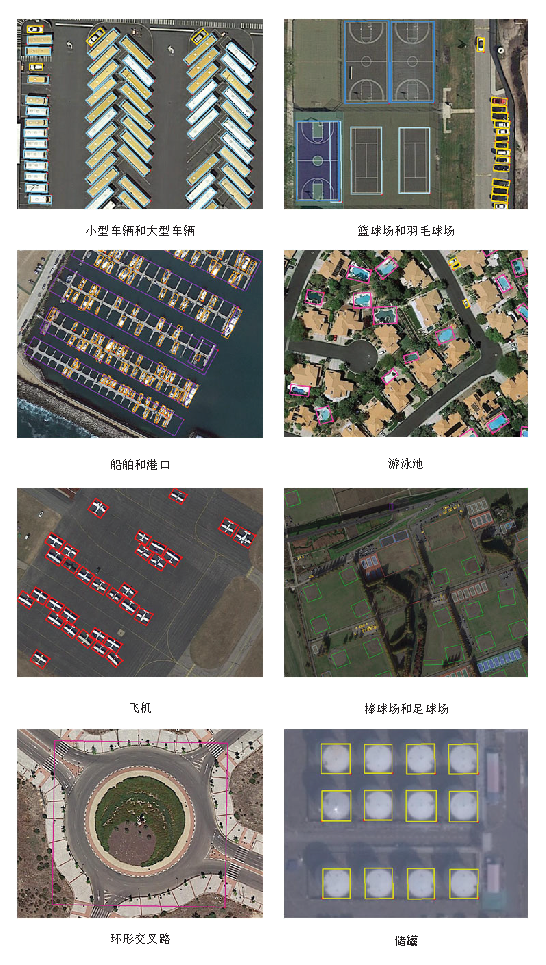
\includegraphics[scale=1.5]{figure/3-8}\caption[短标题]{\label{fig:3-8}本章方法在DOTA数据集上部分类别的检测结果}
%\end{figure}
%
%\clearpage
%
%\begin{figure}
%\centering{}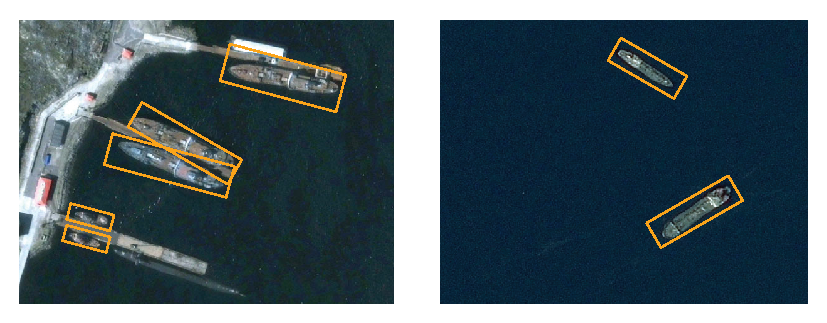
\includegraphics[scale=0.95]{figure/3-9}\caption[短标题]{\label{fig:3-9}本章方法在HRSC2016数据集上的检测结果}
%\end{figure}
%
%
%\section{基于特征对齐和目标长宽比的目标检测方法研究}
%%\section{实验结果与分析}
%%
%%本章实验过程中的运行环境、用到的数据集、实验细节设置以及数据集处理的方式与第三章\ref{3.3.1}和\ref{3.3.2}小节提到的一致,这里就不一一赘述。
%%\subsection{消融实验结果分析}
%%
%为了验证本章设计的多分支特征对齐和基于长宽比的角度偏移损失函数对于算法性能的影响,本小节基于DOTA数据集分别在Faster R-CNN方法和第二章算法的基础上进行了消融实验分析。表\ref{tab:4-1}展示了在Faster R-CNN方法上的实验结果,其中“+DIM”表示添加了多分支特征对齐模块,“+AR-LOSS”表示添加了基于长宽比的角度偏移损失函数。
%
%\begin{table}
%\caption{\label{tab:4-1}Faster R-CNN基础上的消融实验结果}
%
%\centering{}
%\resizebox{\textwidth}{!}{
%\begin{tabular}{c|ccccccccccccccc|c}
%  \hline
%  % after \\: \hline or \cline{col1-col2} \cline{col3-col4} ...
%  & PL & BD & BR & GTF & SV & LV & SH & TC & BC & ST & SBF & RA & HA & SP & HC & mAP\\ \hline
%  Faster R-CNN & 88.25 & 74.84 & 45.45 & 64.55 & 73.61 & 70.59 & 76.97 & 90.83 & 79.39 & 83.44 & 50.78 & 61.06 & 63.16 & 67.28 & 51.68 & 69.95 \\
%  +DIM & 88.74 & 77.55 & 45.77 & 62.19 & 74.02 & 71.56 & 84.17 & 90.86 & 83.07 & 83.67 & 46.70 & 62.38 & 64.00 & 64.59 & 52.78 & 70.33 \\
%  +AR-LOSS & 88.74 & 75.96 & 49.57 & 61.51 & 74.24 & 76.86 & 85.63 & 90.88 & 82.76 & 83.36 & 44.44 & 61.95 & 66.76 & 64.32 & 55.21 & 70.81 \\
%  +Both & 88.78 & 76.54 & 49.89 & 62.11 & 74.42 & 77.22 & 85.83 & 90.91 & 82.84 & 83.89 & 45.56 & 62.45 & 66.92 & 65.00 & 54.89 & 71.15 \\ \hline
%\end{tabular}}
%\end{table}
%
%根据表\ref{tab:4-1}的消融实验对比结果可知,多分支特征对齐模块将检测精度mAP提升了0.38$\%$,在大部分类别上都有一些提升,同时在大目标类别如运动场(GTF)和足球场(SBF)上检测精度有部分下降,大目标是由深层特征来进行检测的,任一特征点表示的范围区域很大,而可形变卷积会在特征点附近任意位置采样,过大的位置偏移会使得采样得到的特征偏离了检测目标,引入了干扰特征,最终影响了检测精度。
%
%添加基于长宽比的角度偏移损失函数将整体的评价指标提升了0.86$\%$ mAP,尤其是在一些大长宽比目标类别上如桥梁(BR)、大型车辆(LV)和港口(HA)有了明显的提升,分别提升了4.12$\%$、6.27$\%$和3.60$\%$ mAP。在有方向目标检测中大长宽比目标对于角度偏移更加敏感,将目标的长宽比作为角度偏移惩罚系数引入到损失函数中可以让模型在训练时更加关注大长宽比目标的角度偏移量学习,有效提升检测精度。
%
%表\ref{tab:4-2}展示了在第二章方法基础上引入本章设计的两个模块得到的消融实验结果,从结果可以得到,将第二章算法和多分支特征对齐一起使用时可以得到0.85$\%$ mAP的提升,相比于在Faster R-CNN基础上的0.38$\%$ mAP有了更明显的提升,这是由于第二章算法中的两级检测结构的缘故,第一级检测结构将感兴趣区域从水平转变为具有一定方向的区域,所带来的的特征不对齐问题相比于Faster R-CNN中更加严重。角度偏移损失函数带来的提升有0.34$\%$ mAP,低于直接在Faster R-CNN上使用得到的0.86$\%$ mAP提升,可以认为第二章算法的两级检测结构先通过一层检测网络完成了对有方向目标位置的初步定位,获得了具有一定方向的检测框参数,在一定程度上缓解了第二级检测网络需要预测的角度偏移量。最后将两个模块全部添加到第二章算法,也就是本章的最终算法,得到了74.37$\%$ mAP的检测精度,相比第二章的方法提升了1.15$\%$。图\ref{fig:4-6}展示了本章的算法和Faster R-CNN算法在DOTA数据集里的各个类别的检测结果。
%
%\begin{table}
%\caption{\label{tab:4-2}第二章算法基础上的消融实验结果}
%
%\centering{}
%\setlength{\tabcolsep}{6mm}{
%\scriptsize
%\begin{tabular}{c|c|cccc}
%  \hline
%  & Faster R-CNN & \multicolumn{4}{c}{不同模块之间设置} \\ \hline
%  %\midrule
%  第二章方法     &          & $\surd$      & $\surd$        & $\surd$        & $\surd$       \\
%  DIM     &          &            & $\surd$         &           & $\surd$        \\
%  AR-LOSS &          &            &               & $\surd$         & $\surd$         \\ \hline
%  %\bottomrule
%  mAP     & 69.95    & 73.22      & 74.07     & 73.56     & 74.37 \\ \hline
%\end{tabular}}
%\end{table}
%
%
%\begin{figure}
%\centering{}\includegraphics[scale=0.8]{figure/4-6}\caption[如果图题太长,在这里写个短标题只在图索引中出现]{\label{fig:4-6}本章方法和Faster R-CNN方法在DOTA数据集各个类别检测结果对比}
%\end{figure}
%
%\subsection{对比实验结果分析}
%
%和第二章提到的一样,在对比实验中选用了RRPN、RoI Trans、R2CNN++、SCRDet和R$^3$Det这5种算法。另外在本章的DOTA对比实验中采用了多尺度训练的方式来适应DOTA数据集中的目标尺度差异大的问题,训练阶段对切分好的数据集图片进行三种尺度的变化(0.5、1.0和1.5),每一张图片扩充到了不同尺度的三张,也相当于进行了数据增强,最终得到的训练图片有20337张。各种方法在DOTA数据集上的对比实验结果如表\ref{tab:4-3}所示,*表示的是进行了多尺度训练,表中加黑突出显示了各个类别的最佳检测精度,从表中的结果可以看到,本章算法在使用更为简单的特征提取模型ResNet-50可以达到74.37$\%$ mAP,相比之前的SCRDet提升了1.76$\%$;使用ResNet-101达到了74.92$\%$ mAP,提升了2.23$\%$。同时在多尺度训练的策略下,使用ResNet-50和ResNet-101分别取得了77.22$\%$和79.76$\%$ mAP,检测精度相对于其他方法有了明显的提升。本章提出的方法主要针对特征不对齐和大长宽比目标检测性能不佳的问题进行研究,实验结果表示本章的方法在一些密集分布以及较大长宽比类别如桥梁(BR)、小型车辆(SV)、大型车辆(LV)、轮船(SH)和港口(HA)上相比于其他方法有明显的提升,验证了该方法的有效性。图\ref{fig:4-7}展示了本章方法在DOTA数据集上的检测结果,最终的结果仍然会存在误检情况,如图\ref{fig:4-7}中将直升机的尾翼误检为飞机类别。
%
%\begin{table}
%\caption{\label{tab:4-3}不同方法在DOTA数据集上的实验结果}
%
%\centering{}%
%\resizebox{\textwidth}{!}{
%\begin{tabular}{c|c|ccccccccccccccc|c}
%  \hline
%  % after \\: \hline or \cline{col1-col2} \cline{col3-col4} ...
%  Methods & Backbone & PL & BD & BR & GTF & SV & LV & SH & TC & BC & ST & SBF & RA & HA & SP & HC & mAP\\ \hline
%  R-DFPN\cite{yang2018automatic} & R-101-FPN & 88.52 & 71.20 & 31.66 & 59.30 & 51.85 & 56.19 & 57.25 & 90.81 & 72.84 & 67.38 & 56.69 & 52.84 & 53.08 & 51.94 & 53.58 & 61.01 \\
%  RoI Trans\cite{ding2019learning} & R-101-FPN & 88.64 & 78.52 & 43.44 & 75.92 & 68.81 & 73.68 & 83.59 & 90.74 & 77.27 & 81.46 & 58.39 & 53.54 & 62.83 & 58.93 & 47.67 & 69.56 \\
%  R2CNN++\cite{yang2018r2cnn++} & R-101-FPN & 89.66 & 81.18 & 45.50 & 71.02 & 67.42 & 59.18 & 66.83 & \textbf{90.90} & 79.00 & 84.43 & 61.17 & 63.48 & 65.34 & 68.01 & 62.05 & 71.09 \\
%  SCRDet\cite{yang2019scrdet} & R-101-FPN & \textbf{89.98} & 80.65 & 52.09 & 68.36 & 68.36 & 60.32 & 72.41 & 90.85 & \textbf{87.94} & \textbf{86.86} & 65.02 & \textbf{66.68} & 66.25 & 68.24 & 65.21 & 72.61 \\
%  R$^3$Det\cite{yang2019r3det} & R-101-FPN & 89.54 & 81.99 & 48.46 & 62.52 & 70.48 & 74.29 & 77.54 & 90.80 & 81.39 & 83.54 & 61.97 & 59.82 & 65.44 & 67.46 & 60.05 & 71.69 \\
%  Ours & R-50-FPN & 88.57& 80.95 & 53.67 & 70.42 & 78.24 & 77.07 & 87.16 & 90.12 & 84.80 & 82.75 & 55.43 & 64.57 & 74.33 & 68.78 & 58.69 & 74.37 \\
%  Ours & R-101-FPN & 88.88 & 82.13 & 52.85 & 69.76 & 78.21 & 77.32 & 87.08 & 90.86 & 86.40 & 82.66 & 56.73 & 65.15 & 74.43 & 68.24 & 63.18 & 74.92 \\
%  Ours* & R-50-FPN & 88.87 & \textbf{86.26} & 55.36 & 72.73 & 79.27 & 77.79 & 87.28 & 90.65 & 85.90 & 86.39 & 60.95 & 66.43 & 77.64 & 72.30 & 70.47 & 77.22 \\
%  Ours* & R-101-FPN & 88.28 & 85.74 & \textbf{59.79} & \textbf{77.46} & \textbf{79.48} & \textbf{84.02} & \textbf{88.32} & 90.82 & 87.45 & 85.65 & \textbf{66.80} & \textbf{66.68} & \textbf{78.78} & \textbf{82.52} & \textbf{74.70} & \textbf{79.76} \\
%  \hline
%\end{tabular}}
%\end{table}
%
%\begin{figure}
%\centering{}\includegraphics[scale=1.2]{figure/4-7}\caption[短标题]{\label{fig:4-7}DOTA数据集部分类别检测结果}
%\end{figure}
%
%表\ref{tab:4-4}中展示了几种不同方法在HRSC2016数据集上的表现,由于数据集中的船舶类别长宽比相对较大,相较于其它方法,本章方法的检测精度比R$^3$Det提升了0.82$\%$,达到了90.08$\%$ mAP。图\ref{fig:4-8}是本章方法在HRSC2016数据集上的部分检测结果展示。
%
%\begin{table}
%\caption{\label{tab:4-4}不同方法在HRSC2016数据集上的表现}
%
%\centering{}%
%\setlength{\tabcolsep}{5mm}{
%%\resizebox{\textwidth}{!}{
%\scriptsize
%\begin{tabular}{c|cccccc}
%  \hline
%  Methods & R-DFPN\cite{yang2018automatic} & RoI Trans\cite{ding2019learning} & R2CNN++\cite{yang2018r2cnn++} & SCRDet\cite{yang2019scrdet} & R$^3$Det\cite{yang2019r3det}  & Ours\\ \hline
%  mAP & 79.08 & 86.20 & 87.40 & 88.21 & 89.26 & \textbf{90.08}\\
%  \hline
%\end{tabular}}
%\end{table}
%
%\begin{figure}
%\centering{}\includegraphics[scale=1.4]{figure/4-8}\caption[短标题]{\label{fig:4-8}HRSC2016数据集检测结果}
%\end{figure}
%
%
%\section{改进的深度级联遥感目标检测网络}
%\subsection{实验细节}
%
%(1)实验参数设置:本次实验使用Faster-RCNN作为基准网络,加入FPN、可形变卷积与三级的级联网络,在DOTA1.5数据集上进行实验,实验使用数据格式为COCO格式;
%
%(2)网络参数设置:图像标准化使用的三通道均值为[123.675, 116.28, 103.53],方差为[58.395, 57.12, 57.375],batch的大小为2,优化算法为随机梯度下降算法(Stochastic Gradiend Descent, SGD),初始学习率设置为0.0025,训练周期为12个epoch,所使用实验网络模型与实验结果都使用ResNet-50-FPN作为骨干网络的特征提取结构。
%
%\subsection{实验结果与分析}
%
%首先将从backbone的ResNet-50中获取的特征图进行可视化并绘制成热力图,并映射至原图像当中,如图\ref{F15}所示,(a)是使用标准卷积核卷积得到的四阶段卷积特征图可视化结果,(b)是加入了可形变卷积后得到的同样四阶段卷积特征图可视化结果,其中从左至右卷积阶段逐渐深入,分别对应着不同尺度下的网络响应情况。可以发现,在未加入可形变卷积模块前,热力图中普遍有许多背景部分具有较高的响应,较为明显的体现有Conv4\_x、Conv5\_x中图像中间部分,原本是停车场的空旷地区,却具有明显地热度响应,当加入可形变卷积之后,显著降低了这一部分背景的干扰,增强了在周围街道、边缘等目标密集区域的响应。说明可形变卷积在遥感图像的特征提取过程中具有较好的表现。
%
%\begin{figure}
%  \centering
%  \includegraphics[scale=0.7]{figure/F15}
%  \caption{特征图可视化}\label{F15}
%\end{figure}
%
%接下来,设计消融对比实验,分别设置5组实验网络,以Faster RCNN网络作为基础对照组,分别加入可形变卷积模块、级联结构及两模块组合,同时,为了增加实验可信度与可参照性,还额外使用了RetinaNet网络结构在同等设置参数条件下进行检测,最终得到检测结果如表\ref{table1}所示,同一指标下最优结果已使用粗体标出,可以发现当同时使用可形变卷积与级联结构时,网络取得了最好表现,在小目标上的检测精度相比于基础对照组有了显著提升,在AP[small]指标下,同时使用了级联结构与可形变卷积的网络与只使用可形变卷积的网络具有接近的性能,且这一指标值远大于其他没有使用可形变卷积的网络检测结果,这突出体现了可形变卷积对于细节特征提取和小目标检测的提升能力。同时在IoU为0.75时,级联网络也取得了远好于非级联网络的结果,这证明了级联网络在遥感目标检测网络中的有效性。
%\begin{table}\small
%
%\caption{\label{table1}检测结果}
%
%\centering{}%
%\setlength{\tabcolsep}{1mm}{
%\begin{tabular}{c|c|c|c|c|c|c}
%\hline
%算法 &AP[0.5:0.95] & AP[0.5] & AP[0.75] & AP[small] & AP[medium] & AP[large]\tabularnewline
%\hline
%Faster-RCNN(base) & 0.330 & 0.550 & 0.343 & 0.236 & 0.266 & 0.402\tabularnewline
%
%base+Cascade & 0.414 & 0.635 & 0.448 & 0.289 & 0.441 & 0.520\tabularnewline
%
%base+DCN & 0.405 & 0.650 & 0.431 & \textbf{0.305} & 0.439 & 0.503\tabularnewline
%
%base+DCN+Cascade & \textbf{0.421} & \textbf{0.651} & \textbf{0.450} & 0.304 & \textbf{0.442} & \textbf{0.531}\tabularnewline
%
%RetinaNet & 0.384 & 0.645 & 0.401 & 0.194 & 0.404 & 0.484\tabularnewline
%\hline
%\end{tabular}}
%\end{table}
%
%\begin{figure}
%  \centering
%  \includegraphics[scale=0.7]{figure/F16.eps}
%  \caption{训练损失曲线}\label{F16}
%\end{figure}
%最后,针对设置的对照网络,记录其训练损失并进行分析,其损失曲线如图\ref{F16}所示,训练损失曲线可以体现出网络在训练过程中的运行状态,是用于评价网络性能的常用指标,在通常情况下,随着网络训练过程的深入,训练计算得到的预测损失虽然存在样本间波动,但整体趋势体现为逐渐减小。显然的,在(a)图使用Faster-RCNN和(b)图加入可形变卷积的网络损失曲线中,在训练多个epoch后,曲线出现了一次较大震荡,随后损失骤降,且结合准确率进行验证后发现,此时已经出现一定的过拟合现象,虽然训练损失降低了,但其泛化性能却因此变差,这限制了网络的检测上限;而(c)图和(d)都加入了三级级联结构,此时损失曲线平滑降低,不再出现跳跃式震荡,说明级联结构的加入的确有效预防了网络过拟合现象的出现,可以允许网络进行更深的训练和对目标位置更加敏感的学习以获得更优检测效果。
%
%上述实验结果表明,加入的可形变卷积结构与级联网络确能提升网络在遥感图像中的目标检测准确率,且避免了训练过程中过拟合问题的出现。基于Faster-RCNN的改进可形变卷积的深度级联遥感目标检测网络在实验中获得了最优表现,相较于原始检测网络与现有的部分方法有了明显提升。
%
%\section{基于GSD预测的超分辨遥感目标检测网络}
%\subsection{实验预处理}
%
%在实验前,由于GSD预测网络无法直接使用DOTA训练集进行学习,因此对所使用数据集进行自定义,生成具有地面采样距离信息的遥感图像数据集,为预测网络提供样本。首先筛选出训练集中已有标注GSD信息的遥感图像,统计其值分布情况如图\ref{F26}所示,可以发现,图像的GSD大多集中分布于小数值区域,而大数值的图像数量较少,样本分布平衡性不足,因此在挑选出图像之后,选取其中的大地面采样距离数值图像进行图像增广,主要增广方法为将这些图像进行分割、镜像、旋转等无形变的处理,最后以特定的数值作为分割标准,将大于这一数值的遥感图像归入大GSD图像类别,小于这一数值的图像属于正常GSD范围图像。同时,从训练集中额外选取若干具有较大GSD的图像,经由同样增广处理后将其作为测试集使用,得到图像测试集D1,D2,其中D1具有145张多尺度图像,D2 具有164张多尺度图像,D1、D2中所有图像的GSD值均大于4。
%\begin{figure}
%  \centering
%  \includegraphics[scale=0.5]{figure/F26}
%  \caption{DOTA1.5数据集GSD分布}\label{F26}
%\end{figure}
%
%与SRGAN相同,超分辨网络基于VGG54预训练模型进行训练,用以训练生成器的低分辨率图像与高分辨率图像来自RAISE数据集中,共计有8156张,具体处理方式为,将数据集中的原始raw格式图像进行5倍下采样,并转换为png格式得到高分辨率图像;同样再对高分辨率图像进行4倍下采样得到低分辨率图像。
%
%\subsection{实验细节}
%
%1.GSD预测网络输入尺度设置:GSD预测网络需要输入完整的遥感图像提取纹理信息进行预测,但出于降低资源消耗与减少计算复杂度的目标,应当避免使用原图尺寸进行输入,基于数据集处理特性与网络连续性考虑,在确保输入纹理信息不产生畸变的前提下将输入尺度大小设定为448×448;
%
%2.超分辨网络参数设置:在本实验中,将GSD1.0作为大GSD图像与正常GSD图像的分界线,经由统计得知图像中最大GSD为4.5,因此设置超分辨网络放大倍数为4,其具体操作细节设置为,对于输入网络的遥感图像,将其按步长128进行分割,分割大小为200×200,随后在经过超分辨后,得到800×800的具有强边缘的超分辨图像;
%
%3.正常GSD图像分割:在GSD预测网络中,当输入图像被判断具有正常GSD时,不再需要进行额外的超分辨操作,因此直接对其进行裁切,以544为步长,将遥感图像裁切为800×800大小的图像序列依次送往网络检测。
%
%\subsection{实验结果与分析}
%
%实验首先针对GSD预测网络进行检验,如表\ref{table2}所示给出了当使用不同的分类门限λ时,GSD预测网络真正例数(True Positive, TP)、真反例数(True Negative,TN)、假正例数(False Positive, FP)与假反例数(False Negative, FN)的变化,以大于门限值的样本为正例,其余为反例。显然的,当λ=0和λ=4.5时,此时所有图像样本都被归为一类,网络不再具有分辨能力,当λ=0.3时,由于在0.3周围分布有许多图像,且遥感图像的特性决定了GSD在0.3上下时图像纹理差异较为模糊,导致网络将大量GSD值低于0.3的负样本预测为正,其负样本检测准确率降低,同理当λ=2.5时,由于图像区分度不足,网络将许多大于2.5的正样本预测为负,其正样本检测准确率降低;而当λ=1.0时,其FP与FN较小,即意味着在1.0的分类门限下,网络对遥感图像GSD的分布预测更为准确,这与训练使用数据集中的遥感图像分布情况相吻合,在GSD大于1.0的图像中,遥感目标数量显著增长,且在经过图像筛选与数据增广之后,大GSD图像与小GSD图像在1.0边界上分离明显不易混淆,因此更易于区分。
%\begin{table}\small
%
%\caption{\label{table2}不同门限下的混淆矩阵}
%
%\centering{}%
%\setlength{\tabcolsep}{3mm}{
%\begin{tabular}{c|c|c|c|c}
%\hline
%λ & TP & FP & TN & FN \tabularnewline
%\hline
%0 & 1048 & 79 & 0 & 0 \tabularnewline
%0.3 & 757 & 168 & 94 & 108 \tabularnewline
%1 & 702 & 82 & 297 & 46 \tabularnewline
%2.5 & 387 & 148 & 492 & 100 \tabularnewline
%4.5 & 0 & 0 & 1101 & 26 \tabularnewline
%\hline
%\end{tabular}}
%\end{table}
%
%随后,以第三章中设计的改进的深度级联遥感目标检测网络为base,与本章所提出的基于GSD预测的超分辨遥感目标检测网络进行对比如表\ref{table3}所示。可以发现,在使用了GSD预测和超分辨处理SR后,网络检测能力有明显提升,尤其是针对小目标检测任务具有良好表现,AP[small]的提升较之其尺度AP提升更高,对总AP均值的影响也是最大的。
%
%\begin{table}\small
%
%\caption{\label{table3}与深度级联网络的对比结果}
%\centering{}%
%\setlength{\tabcolsep}{0.5mm}{
%\begin{tabular}{c|c|c|c|c|c|c}
%  \hline
%算法 & AP[0.5:0.95] & AP[0.5] & AP[0.75] & AP[small] & AP[medium] & AP[large] \tabularnewline
%\hline
%Faster-RCNN & 0.330 & 0.550 & 0.343 & 0.236 & 0.366 & 0.402 \tabularnewline
%Faster-RCNN+Cascade+DCN & 0.421 & 0.651 & 0.45 & 0.304 & 0.442 & 0.531 \tabularnewline
%GSD+GAN & \textbf{0.445} & \textbf{0.694} & \textbf{0.473} & \textbf{0.412} & \textbf{0.448} & \textbf{0.534} \tabularnewline
%RetinaNet & 0.384 & 0.645 & 0.401 & 0.194 & 0.404 & 0.484 \tabularnewline
%  \hline
%\end{tabular}}
%
%\end{table}
%
%为了进一步检验本章节所设计网络在大GSD图像中的检测能力,使用前述大GSD数据集D1、D2进行消融实验,得到其检测结果如表\ref{table4}所示,其中base为第三章中所提出的改进的级联卷积网络,GSD为本章提出的GSD预测方法,SR为本章使用的超分辨方法。由D1和D2数据集测试数据可以看出,相较于没有针对性GSD设计的base方法,GSD预测超分辨网络对于大GSD目标检测准确率提升明显。同时,在D2上进行的消融实验证明,当仅仅使用双线性插值方法代替超分辨网络时,检测结果相较于base仍有提升,但对比加入超分辨GAN的网络又略显落后,这证明了GSD预测思路的有效性,同时也说明了超分辨网络比传统插值方法在遥感图像处理中具有优势。如图\ref{F27}所示分别为D2上消融实验的输入示例,图(a)为未使用GSD预测时,大GSD图像直接输入网络的情形,图(b)与图(c)都使用了GSD预测网络,区别在于图(b)使用了双线性插值方法将图像放大四倍,而(c)则使用了超分辨网络进行放大,显然的,图(c)中目标具有较好的可视性。
%
%\begin{table}\small
%  \centering
%  \caption{在大GSD数据集上的检测结果}\label{table4}
%  \begin{tabular}{c|c|c|c|c}
%    \hline
%    % after \\: \hline or \cline{col1-col2} \cline{col3-col4} ...
%    算法 & AP[0.5:0.95] & AP[0.5] & AP[0.75] & AR[0.5:0.95] \\
%    \hline
%    base(D1) & 0.240 & 0.406 & 0.236 & 0.272 \tabularnewline
%
%    base+GSD+SR(D1)& 0.317 & 0.589 & 0.268 & 0.405 \tabularnewline
%    base(D2) & 0.252 & 0.433 & 0.252 & 0.309 \\
%    base+GSD(D2) & 0.310 & 0.550 & 0.281 & 0.367 \\
%    base+GSD+SR(D2) & \textbf{0.326} & \textbf{0.649} & \textbf{0.295} & \textbf{0.416} \\
%    \hline
%  \end{tabular}
%
%\end{table}
%\begin{figure}
%  \centering
%  \includegraphics[scale=0.7]{figure/F27.eps}
%  \caption{网络输入图像}\label{F27}
%\end{figure}
%\begin{figure}
%  \centering
%  \includegraphics[scale=0.8]{figure/F28.eps}
%  \caption{检测结果}\label{F28}
%\end{figure}
%
%再取实验检测结果进行可视化,如图\ref{F28}所示,在图(a)示例当中,原图像右下角存在大量存储罐(Storage Tank)类目标,由于在原图中尺度过小难以被检出,在经过GSD预测超分辨后能完全检测出所有目标;而在图(b)示例中,左上方区域右上角的存储罐目标同样由于尺度太小难以被检出,经过超分辨后能够被精确检测,同时在右下方机场区域存在大量飞机(Plane)类别目标,在原始图像中有10个目标被检测到,还有两个目标由于检测框重叠没有被准确检测到,在经过超分辨后,其定位精确性与检测率均有提升,能成功检测到所有的12个目标,减少了目标遗漏现象。

\chapter{总结}

本文为中科院太空应用重点实验室开放基金课题的研究报告,以多尺度遥感图像目标自动检测与识别技术作为研究的核心要点,从四个方向分别对遥感图像的尺度多样性问题、多方向问题、小目标问题及视角特殊性问题给出了对应的解决方案,搭建并完善出具有适应性、针对性的遥感图像目标检测网络,有效地提升了算法的整体检测精度;具体可以总结为以下五点:

(1)考虑到自然图像中的水平框目标检测方法在对密集分布且方向任意的目标进行检测时容易出现的漏检和虚警问题,在研究过程中采用了有方向框来定位遥感图像中的目标,有方向框可以更好的说明相邻目标检测框之间的相似程度。

(2)提出了一种改进的多方向两级级联R-CNN方法来更好的检测遥感图像中的有方向小目标。在第一级检测网络设计了多方向RoI对齐模块从多个不同旋转方向的感兴趣区域获取方向敏感特征,同时在回归分支添加方向注意力模块自适应地给每个方向通道的特征赋予权重,增强了特征的方向敏感性,然后第一次回归得到初始的可能包含目标的有方向框,这样的有方向框可以更好的表示密集分布的目标的特征。最后在第二级检测网络对该有方向框做进一步回归得到目标的精确位置。

(3)基于区域提取的目标检测方法在检测过程中由于候选区域位置的变化造成了特征不对齐问题,针对这一问题,设计了基于可形变卷积的多分支特征对齐模块来重新采样特征,同时采用了不同扩张率的空洞卷积来获取不同尺度的感受野。另外针对在研究过程中发现的网络模型对于不同长宽比目标的检测倾向不一致问题,提出了基于目标长宽比的角度偏移惩罚损失函数,在训练过程中更加关注大长宽比目标角度偏移量的学习。

(4)设计了一种改进的深度级联遥感目标检测网络,通过分析遥感图像中的目标特点,以通用目标检测中Faster-RCNN的两步法结构为基础架构,加入能有效提取多尺度特征的特征金字塔结构,以残差网络ResNet-50为基础,利用可形变卷积改进特征提取过程,并在最终目标检测网络中适用了一种三级级联结构,避免网络学习中过拟合现象的出现,同时提高了检测IoU门限。使得改进后的网络能够更加全面地利用遥感图像中多尺度信息进行检测,增强了对小目标的检测和定位能力;

(5)以遥感图像中额外具有的地面采样距离信息GSD为基础,研究并提出了一种基于遥感图像GSD的超分辨遥感目标检测方法。其主要思路是利用遥感图像覆盖范围广、区域纹理丰富的特性,将图像复杂度估计方法与遥感图像GSD相关联,将其作为额外信息引入目标检测网络,同时利用超分辨网络结合GSD对图像进行选择性放大,最终达到使具有大GSD的图像中较难以被检测到的密集小型目标被放大至更合适的尺度的效果,进而提升遥感图像中小目标密集区域的检测效率与准确率。

\bibliographystyle{scutthesis}
\bibliography{scutthesis}
%\bibliography{scutthesis1}
\end{document} 